\documentclass[output=paper,colorlinks,citecolor=brown,portuguese]{langscibook} 

%dependencias para desenhar árvores sintáticas
\usepackage{tikz}
\usepackage{tikz-dependency}
%\usepackage{python}
%\usepackage{minted} %\begin{minted}{python}
\usepackage{longtable}
%\usepackage{biblatex}

%nome da section no header de cada página
%\usepackage{fancyhdr}
%\pagestyle{fancy}
%\fancyhf{}
%\fancyhead[L]{\rightmark}
%\fancyhead[R]{\thepage}
%\renewcommand{\headrulewidth}{0pt}
\usepackage{dirtytalk}
\usepackage{float}

\bibliography{localbibliography.bib}
%\addbibresource{localbibliography.bib}

\newcommand*{\fullref}[1]{\hyperref[{#1}]{\autoref*{#1}: \nameref*{#1}}} % One single link
\setcounter{secnumdepth}{5}
\setcounter{tocdepth}{5}

\author{Elvis de Souza\and Tatiana Cavalcanti\and Aline Silveira\and Wograine Evelyn\and Cláudia Freitas}
\title{Diretivas e documentação\\
de anotação UD em português\\
(e para língua portuguesa)}

\abstract{Versão 1.3 - 26/10/2020\newline Baseadas nas diretivas originais do Projeto Universal Dependencies\newline\newline
O projeto Universal Dependencies \citep{mcdonald2013universal} apresenta um tagset e uma gramática. Isso significa dizer que, para além de um conjunto de etiquetas que correspondem às classes da Gramática Tradicional (objeto, sujeito etc.), o UD também faz diversas escolhas que diferem da GT. Nesse documento, apresentamos a documentação detalhada e as escolhas linguísticas relativas ao processo de revisão do material UD em Português. Considerando que UD funciona como uma espécie de segunda língua gramatical, partimos, sempre que possível, das categorias e análises de GT, e não de UD, para facilitar a consulta.

As diretivas originais, em inglês, estão disponíveis na página do projeto e devem ser consultadas também: \href{https://universaldependencies.org/guidelines.html}{https://universaldependencies.org/guidelines.html}

Este documento não pretende ser uma substituição das diretivas originais, mas um complemento, por um lado, e um detalhamento, por outro, no que se refere à língua portuguesa.
}

% add all extra packages you need to load to this file  
\usepackage{tabularx} 

%%%%%%%%%%%%%%%%%%%%%%%%%%%%%%%%%%%%%%%%%%%%%%%%%%%%
%%%                                              %%%
%%%           Examples                           %%%
%%%                                              %%%
%%%%%%%%%%%%%%%%%%%%%%%%%%%%%%%%%%%%%%%%%%%%%%%%%%%% 
%% to add additional information to the right of examples, uncomment the following line
% \usepackage{jambox}
%% if you want the source line of examples to be in italics, uncomment the following line
% \renewcommand{\exfont}{\itshape}
\usepackage{langsci-optional}
\usepackage{langsci-gb4e}  
\makeatletter
\let\thetitle\@title
\let\theauthor\@author 
\makeatother

\newcommand{\togglepaper}[1][0]{ 
%   \bibliography{../localbibliography}
  \papernote{\scriptsize\normalfont
    \theauthor.
    \thetitle. 
    To appear in: 
    Change Volume Editor \& in localcommands.tex 
    Change volume title in localcommands.tex
    Berlin: Language Science Press. [preliminary page numbering]
  }
  \pagenumbering{roman}
  \setcounter{chapter}{#1}
  \addtocounter{chapter}{-1}
}

\begin{document}

\maketitle

\addtocontents{toc}{\protect\hypertarget{toc}{}}

\tableofcontents

\chapter{Formato UD}\label{sec:formatoud}

\hyperlink{toc}{Ir para tabela de conteúdos\\}

Os treebanks adaptados para a gramática UD são disponibilizados no formato CoNLL-U, em que há um token por linha. Cada anotação de cada token, por sua vez, é disposta em uma coluna, sendo 10 colunas ao todo. Cada token tem a configuração conforme a \fullref{tab:colunasUD}, com uma tabulação (\textit{Tab}) separando as colunas.

Colunas sem nenhum valor devem, necessariamente, ser preenchidas com \textit{underline}, conforme diretivas da página do \href{https://universaldependencies.org/format}{formato CoNLL-U} (acesso em 28 de outubro de 2019).

\begin{table}
    \centering
    \begin{tabular}{c c c c c c c c c c}
        id & word & lemma & upos & xpos & feats & dephead & deprel & deps & misc\\
    \end{tabular}
    \caption{Colunas do formato UD 2.0}
    \label{tab:colunasUD}
\end{table}

\section{Colunas/anotações}\label{sec:colunas}

\begin{enumerate}
    \item “id” corresponde ao número do token, em ordem crescente;
    \item “word”, à palavra tal como aparece na frase (exceto no caso de contração, como “da”, em que a palavra será desmembrada nos tokens “de” e “a”);
    \item “lemma” se refere à palavra tal como aparece no dicionário: em singular e em masculino ou infinitivo;
    \item “upos” (classe gramatical \say{universal}) se refere à classe gramatical;
    \item No corpus Bosque-UD, a coluna “xpos” (classe gramatical específica) é preenchida com a saída do sistema PALAVRAS \citep{bick2000parsing} para a mesma frase. No entanto, essa coluna é removida na versão que é tornada pública (release);
    \item “feats” (atributos morfológicos) é preenchida com as características morfológicas do token;
    \item “dephead” (dependência sintática), com o id do token de quem é filho. Indica a relação estrutural de dependência entre os elementos de um enunciado; 
    \item “deprel” (relação de dependência), com a relação sintática que o conecta ao seu pai.  Indica a natureza, isto é, o tipo de relação sintática entre os elementos de um enunciado;
    \item “deps” (dependência específica) não é utilizado no Bosque-UD;
    \item “misc” (miscelânea) se refere a quaisquer informações extras que se queira adicionar ao token.
\end{enumerate}{}

\section{Princípios}\label{sec:principios}

	De \href{https://universaldependencies.org/introduction.html}{Página do Universal Dependencies} (acesso em 28 de outubro de 2019).
	
	What is needed for UD to be successful?
	The secret to understanding the design and current success of UD is to realize that the design is a very subtle compromise between approximately 6 things:
	
	\begin{enumerate}
		\item UD needs to be satisfactory on linguistic analysis grounds for individual languages.
		\item UD needs to be good for linguistic typology, i.e., providing a suitable basis for bringing out cross-linguistic parallelism across languages and language families.
		\item UD must be suitable for rapid, consistent annotation by a human annotator.
		\item UD must be suitable for computer parsing with high accuracy.
		\item UD must be easily comprehended and used by a non-linguist, whether a language learner or an engineer with prosaic needs for language processing. We refer to this as seeking a habitable design, and it leads us to favor traditional grammar notions and terminology.
		\item UD must support well downstream language understanding tasks (relation extraction, reading comprehension, machine translation, …).
	\end{enumerate}


\chapter{Para começar...}\label{sec:paracomecar}

	\hyperlink{toc}{Ir para tabela de conteúdos\\}

	Listamos aqui alguns pontos que podem causar surpresa para quem não é familiarizado com dependências sintáticas e/ou com UD:
	
	\begin{enumerate}
		\item O núcleo da oração é sempre um verbo. E quando estamos tratando de núcleo da oração principal, ele é o \emph{root}. EXCEÇÃO: Quando estivermos diante de um verbo de ligação como \say{ser} e, em alguns contextos, \say{estar}, eles NÃO SERÃO NÚCLEOS. Nesses casos, o núcleo é o elemento predicado/predicativo (em geral, um substantivo ou adjetivo). Apenas o verbo \say{ser}, e algumas ocorrências de \say{estar} (\say{estar feliz}, mas não \say{estar na praia}) são considerados auxiliares em UD. 

		\item Preposições: Estamos habituados a atrelar as preposições às palavras que as antecedem: em \say{gostar de sorvete}, o \say{de} depende (isto é,  \say{é filho sintático}) de  \say{gostar}; em \say{casa de madeira}, o \say{de} depende de \say{casa}. Em UD, as preposições dependem do elemento que está à direita. Assim, em \say{gostar de sorvete}, o \say{de} depende de \say{sorvete} — e \say{sorvete}, por sua vez, depende de \say{gostar}; em \say{casa de madeira}, o \say{de} depende de \say{madeira} — e \say{madeira}, por sua vez, depende de \say{casa}. 

		\item Conjunções: a mesma coisa que preposições. Em \say{gato e sapato}, o \say{e} depende de \say{sapato}; e \say{sapato} depende de \say{gato}.

		\item \textbf{Algumas palavras sobre o Bosque-UD}

		A maioria dos exemplos compilados nessa documentação vem do corpus Bosque-UD, que é uma conversão, para o modelo UD, do corpus Bosque, seguido de algumas rodadas de revisão. O corpus Bosque, por sua vez, foi tornado público pela primeira vez em 2002 \citep{santos2002floresta}, como parte do projeto Floresta Sintá(c)tica (\href{http://www.linguateca.pt/Floresta/}{http://www.linguateca.pt/Floresta/}), coordenado pela Linguateca (\href{http://www.linguateca.pt}{http://www.linguateca.pt}).  Por se tratar de um material revisto, tem sido amplamente utilizado em tarefas de PLN, inclusive no âmbito internacional (por exemplo, o CoNLL 2006), e está disponível em diversos formatos (veja-se a página do projeto).
		
		Em \href{http://www.linguateca.pt/Floresta/documentacao.html}{http://www.linguateca.pt/Floresta/documentacao.html} encontra-se a documentação linguística da anotação do Bosque no âmbito do projeto Floresta Sintá(c)tica, e a construção do presente documento se inspira, também, nesta documentação. 
	\end{enumerate}

\chapter{Lemas}\label{sec:lemas}

	\hyperlink{toc}{Ir para tabela de conteúdos\\}

	O lema é a terceira coluna (ou atributo) no formato CoNLL-U. Lemas não são capitalizados, isto é, devem ter letras minúsculas, exceto pelos nomes próprios (\emph{PROPN}).

	\fullref{tab:lemma}

	\begin{table}[]
	    \centering
	    \begin{tabular}{ c | c }
	    \textbf{upos} & \textbf{lema} \\
          \hline
	    NOUN & o substantivo no singular, não capitalizado \\
	    \hline
	    PROPN & o nome próprio no singular, capitalizado \\
	    \hline
	    ADJ & o adjetivo no masculino singular \\
	    \hline
           VERB & o verbo no infinitivo \\
	    \hline
	    AUX & verbo no infinitivo \\
	    \hline
	    DET & igual aos ADJ \\
	    \hline
	    PRON & se substantivos, devem seguir as diretivas dos \emph{NOUN};\\ & se pronomes adjetivos, dos \emph{ADJ} \\
	    \end{tabular}
	    \caption{Indicação do lema das classes gramaticais variáveis}
	    \label{tab:lemma}
	\end{table}{}

	Os lemas das palavras de classes invariáveis (preposições, conjunções, advérbios) é a própria palavra, em minúscula.


\chapter{Classes gramaticais (upos)}\label{sec:upos}

\hyperlink{toc}{Ir para tabela de conteúdos\\}

São 17 as classes gramaticais em UD. Elas são atribuídas com base no contexto, conforme \fullref{sec:classesdinamicas}.

\fullref{tab:upos}

\begin{longtable}{| p{1.5cm} | p{10cm} | }
    \hline
    ADJ & Adjetivos e numerais ordinais\newline Manchete estréia \textbf{novo} jornalístico\newline É o \textbf{5º} Encontro Nacional de Histórias em Quadrinhos \\
    \hline
    ADP & Preposições\newline «Confissões» chega \textbf{a} Portugal \\
    \hline
    PUNCT & Pontuação\newline \textbf{«}Tem que torcer muito e rezar bastante, porque milagres acontecem\textbf{»}. \\
    \hline
    ADV & Advérbio\newline Outros profissionais brasileiros, que atuam nos EUA, \textbf{também} participam. \\
    \hline
    AUX & Verbos auxiliares e copulativos\newline A direção do novo semanal \textbf{será} assinada por Ewaldo Ruy. \\
    \hline
    SYM & Símbolos\newline BRIZOLA É O 3º No Rio, com 13 \textbf{\%} . \\
    \hline
    INTJ & Interjeição\newline «\textbf{Ah bem}, pensei que voce ia pescar». \\
    \hline
    CCONJ & Conjunção coordenativa\newline Eles se dizem oposição, \textbf{mas} ainda não informaram o que vão combater. \\
    \hline
    NOUN & Substantivo\newline Romário não se exercitou nas \textbf{cobranças} de \textbf{falta} e \textbf{pênalti}. \\
    \hline
    DET & Determinante — artigos e pronomes adjetivos\newline De Mario Bernardini, d\textbf{a} Fiesp, sobre \textbf{a} seleção e \textbf{o} real: \\
    \hline
    PART & Partículas/morfemas livres\newline Esta vertente, francamente conteudista, derivava das experiências realizadas no período \textbf{pré}-64 pelos Centros Populares de Cultura (CPCs), ligados à União Nacional dos Estudantes, que privilegiavam a «mensagem» e procuravam falar uma idealizada linguagem do «povo».\\
    \hline
    PROPN & Nomes próprios, apenas se com inicial maiúscula\newline \textbf{Ilmar Galvão} e \textbf{Moreira Alves} votaram pela concessão do mandato de segurança. \\
    \hline
    NUM & Numerais — exceto os ordinais, que são adjetivos\newline Os \textbf{três} estão presos desde \textbf{30} de julho de \textbf{93}. \\
    \hline
    VERB & Verbo\newline \textbf{Tem} sentido -- aliás, muitíssimo sentido. \\
    \hline
    PRON & Apenas pronomes substantivos\newline \textbf{Ele} só não jogava porque não estava bem. \newline Aqui só joga \textbf{quem} está bem. \\
    \hline
    SCONJ & Conjunções subordinativas\newline Ele só não jogava \textbf{porque} não estava bem.\newline Nem Lula nem o partido ainda encontraram um discurso \textbf{para} se diferenciar. \\
    \hline
    X & No Bosque-UD, palavras estrangeiras\newline A dupla planeja agora temporada de \textbf{dolce far niente}. \\
    \hline
    \caption{As 17 classes gramaticais do UD em português}
    \label{tab:upos}
\end{longtable}

	Nas próximas seções, comentamos apenas casos de classes que podem causar dificuldade. 

\section{A classificação de uma palavra é feita em contexto}\label{sec:classesdinamicas}

	A classe gramatical de uma palavra é sempre dada pelo contexto. Assim, em \emph{Ela joga bonito}, \say{bonito} deve ser um \emph{ADV}, e não um \emph{ADJ}. O mesmo se aplica às palavras gramaticais, como preposições e conjunções (e não à toa a GT tem o conceito de \say{preposição acidental}). Ao longo da anotação, é comum, por exemplo, que uma palavra como \say{para} seja utilizada para introduzir uma oração subordinada adverbial, como em \fullref{dep:classesdinamicas}. Nesse caso, o \say{para} será classificado como uma conjunção subordinativa (\emph{SCONJ}).
		
	\begin{figure}[H]
		\centering
		\vspace{.8cm}
		\begin{dependency}
			\begin{deptext}
				VERB \& DET \& NOUN \& SCONJ \& PRON \& VERB \\
				Encontraram \& um \& discurso \& para \& se \& diferenciar \\
				encontrar \& um \& discurso \& para \& se \& diferenciar \\
			\end{deptext}
			\deproot{1}{root}
			\depedge{1}{3}{nsubj}
			\depedge{3}{2}{det}
			\depedge{6}{4}{mark}
			\depedge{6}{5}{expl}
			\depedge{1}{6}{advcl}
		\end{dependency}
		\caption{Encontraram um discurso \emph{para} se diferenciar}\label{dep:classesdinamicas}
	\end{figure}


\section{Verbos auxiliares e verbo de ligação}\label{sec:verbosauxiliares}

	Verbos auxiliares são classificados como \emph{AUX}. Via de regra, verbos auxiliares (\emph{AUX}) não podem ter dependentes, isto é, filhos sintáticos, e dependem, isto é, são filhos, de um verbo principal (\emph{VERB}). A deprel pode ser \emph{cop}, \emph{aux} ou \emph{aux:pass}, de acordo com a função sintática exercida pelo \emph{AUX} e/ou pela locução verbal.

	O que conta como um verbo auxiliar é alvo de discussão nas gramáticas do português (\citet{elvis2019locverbal}). Em UD, o que algumas GTs consideram locuções verbais aspectuais e modais não são classificadas como locução, ou seja, os verbos são anotados como se constituíssem duas orações distintas (\fullref{sec:auxaspecto}). No entanto, conforme apontado em \citet{elvis2019locverbal}, é possível propor uma anotação que leve em conta a auxiliaridade das locuções verbais aspectuais, a qual não abordaremos aqui.

	\subsection{Verbos de ligação}\label{sec:verbosdeligacao}
	
		Apenas os verbos \say{ser} e \say{estar} são considerados verbos de ligação, e portanto serão sempre anotados como \textit{AUX}. Os demais verbos que a GT costuma elencar como verbo de ligação (\say{parecer}, \say{permanecer}, etc.) são anotados como \textit{VERB}.

		Os verbos de ligação \textit{AUX} terão relação sintática (isto é, deprel) \emph{cop}, e nunca poderão ser núcleo de uma oração nem conter dependentes.

		Na frase em \fullref{dep:serAUX}, o núcleo da oração (\emph{root}) não é o verbo \say{ser}, mas o seu complemento. Se a frase fosse \say{a casa é amarela}, o núcleo da oração seria \say{amarela}. Mas, na frase da figura, o complemento do verbo ser é \say{US\$ 422}. Neste caso, e de maneira arbitrária, \say{US\$} (cuja classe/upos é \emph{SYM}, de símbolo) é o núcleo do valor. Portanto, \say{US\$} é pai de \say{422}. E, porque \say{US\$} é o núcleo de \say{US\$ 422}, ele será o núcleo da oração.  

		\fullref{tab:verbosdeligacao}
		
		\begin{figure}[H]
			\centering
			\vspace{.8cm}
			\begin{dependency}
				\begin{deptext}
					DET \& NOUN \& AUX \& ADP \& SYM \& NUM \\
					O \& preço \& é \& de \& US\$ \& 422 \\
					o \& preço \& ser \& de \& US\$ \& 422 \\
				\end{deptext}
				\depedge{2}{1}{det}
				\deproot{5}{root}
				\depedge{5}{2}{nsubj}
				\depedge{5}{3}{cop}
				\depedge{5}{4}{case}
				\depedge{5}{6}{nummod}
			\end{dependency}
			\caption{O preço \emph{é} de US\$ 422}\label{dep:serAUX}
		\end{figure}


	\subsection{Verbo \textit{ser} como voz passiva}\label{sec:servozpassiva}
		
		A anotação de \say{ser} como voz passiva, além do upos \emph{AUX}, deve receber deprel \emph{aux:pass}.

		Para o fenômeno da voz passiva, ver \fullref{sec:vozpass}.

		\fullref{dep:serPASS}
		
		\begin{figure}[H]
		    \centering
		    \vspace{.8cm}
		    \begin{dependency}
		    \begin{deptext}
		    DET \& NOUN \& AUX \& VERB \& ADP \& DET \& NOUN \\
		    A \& fotografia \& foi \& publicada \& em \& a \& imprensa \\
		    o \& fotografia \& ser \& publicar \& em \& a \& imprensa \\
		    \& \& \& VerbForm=Part \& \& \& \\
		    \end{deptext}
		    \depedge{2}{1}{det}
		    \depedge{4}{3}{aux:pass}
		    \deproot{4}{root}
			\depedge{4}{7}{obl}
		    \depedge{4}{2}{nsubj}
		    \depedge{7}{6}{det}
		    \depedge{7}{5}{case}
		    \end{dependency}
		    \caption{A fotografia \emph{foi} publicada na imprensa}\label{dep:serPASS}
		\end{figure}	

	\subsection{Locuções verbais de tempo composto}\label{sec:auxtempocomposto}

		Segundo as gramáticas, são locuções verbais de tempo composto aquelas que têm como verbo auxiliar \say{ter}, \say{haver} e, para nós, também \say{ir}.

		\fullref{dep:auxtempocomposto}

		\fullref{tab:loctempocomposto}

		\begin{figure}[H]
			\centering
			\vspace{.8cm}
			\begin{dependency}
				\begin{deptext}
					DET \& PROPN \& ADV \& AUX \& VERB \& DET \& NOUN \& PUNCT \\
					A \& Prefeitura \& não \& havia \& retirado \& o \& golfinho \& . \\
					o \& Prefeitura \& não \& haver \& retirar \& o \& golfinho \& . \\
					\& \& Polarity=Neg \& \& \& \& \& \\
				\end{deptext}
				\depedge{2}{1}{det}
				\depedge{5}{3}{advmod}
				\deproot{5}{root}
				\depedge{5}{7}{obl}
				\depedge{5}{2}{nsubj}
				\depedge{7}{6}{det}
				\depedge{5}{7}{obj}
				\depedge{5}{8}{punct}
				\depedge{5}{4}{aux}
			\end{dependency}
			\caption{A Prefeitura não \emph{havia retirado} o golfinho}
			\label{dep:auxtempocomposto}
		\end{figure}


	\subsection{Locuções verbais aspectuais/modais não existem no UD}\label{sec:auxaspecto}
	
		Em UD, não existem locuções verbais aspectuais ou modais, de modo que as sentenças são anotadas como na \fullref{dep:locverbalUD} e \fullref{dep:locverbalUD2}, com dois verbos plenos (\emph{VERB}), sendo o segundo de deprel \emph{xcomp} dependente do primeiro (ver \fullref{sec:objetooracional}).
		
		\begin{figure}[H]
			\centering
			\vspace{.8cm}
			\begin{dependency}
				\begin{deptext}
					DET \& NOUN \& VERB \& VERB \& ADV \& ADP \& PROPN \& PUNCT \\
					A \& seleção \& deve \& contar \& hoje \& com \& Giovane \& . \\
					o \& seleção \& dever \& contar \& hoje \& com \& Giovane \& . \\
				\end{deptext}
				\depedge{2}{1}{det}
				\depedge{4}{5}{advmod}
				\deproot{3}{root}
				\depedge{4}{7}{obl}
				\depedge{7}{6}{case}
				\depedge{3}{2}{nsubj}
				\depedge{3}{8}{punct}
				\depedge{3}{4}{xcomp}
			\end{dependency}
			\caption{A seleção \emph{deve contar} hoje com Giovane}
			\label{dep:locverbalUD}
		\end{figure}
		
		\begin{figure}[H]
			\centering
			\vspace{.8cm}
			\begin{dependency}
				\begin{deptext}
					DET \& PROPN \& AUX \& AUX \& SCONJ \& VERB \& DET \& NOUN \& PUNCT \\
					O \& Tribunal \& vai \& começar \& a \& ouvir \& as \& testemunhas \& . \\
					o \& Tribunal \& ir \& começar \& a \& ouvir \& o \& testemunha \& . \\
				\end{deptext}
				\depedge{2}{1}{det}
				\deproot{4}{root}
				\depedge{6}{8}{obj}
				\depedge{8}{7}{det}
				\depedge{4}{2}{nsubj}
				\depedge{4}{9}{punct}
				\depedge{4}{3}{aux}
				\depedge{4}{6}{xcomp}
				\depedge{6}{5}{mark}
			\end{dependency}
			\caption{O Tribunal vai \emph{começar a ouvir} as testemunhas}
			\label{dep:locverbalUD2}
		\end{figure}
	

	\subsection{Isso \emph{foi} nos Estados Unidos: verbo \textit{ser} como verbo pleno}\label{sec:serpleno}
	
		Atenção para 2 casos em que o \say{ser} não é verbo auxiliar e deve ser verbo pleno (upos \textit{VERB}).
		
		1) Como na \fullref{dep:serVERB}, o \say{ser} deve ser núcleo da oração caso o predicado seja uma outra oração (\textit{ccomp, xcomp}).
		
		\begin{figure}[H]
		    \centering
		    \vspace{.8cm}
		    \begin{dependency}
		    \begin{deptext}
		    DET \& NOUN \& VERB \& SCONJ \& VERB \& ADP \& SYM \& NUM \& NUM \\
		    A \& expectativa \& era \& que \& chegasse \& a \& US\$ \& 7 \& milhões \\
		    o \& expectativa \& ser \& que \& chegar \& a \& US\$ \& 7 \& milhão \\
		    \end{deptext}
		    \depedge{2}{1}{det}
		    \depedge{3}{2}{nsubj}
		    \deproot{3}{root}
		    \depedge{3}{5}{ccomp}
		    \depedge{5}{4}{mark}
		    \depedge{7}{6}{case}
		    \depedge{8}{9}{flat}
		    \depedge{7}{8}{nummod}
		    \depedge{5}{7}{obl}
		    \end{dependency}
		    \caption{A expectativa \emph{era} que chegasse a US\$7 milhões}\label{dep:serVERB}
		\end{figure}
		
		2) \say{ser} verbo intransitivo (verbo pleno) também deve ter a anotação \textit{VERB}, como na \fullref{dep:serVERB2}.
		
		\begin{figure}[H]
			\centering
			\vspace{.8cm}
			\begin{dependency}
				\begin{deptext}
					PRON \& VERB \& ADP \& DET \& PROPN \& PROPN \\
					Isso \& foi \& em \& os \& Estados \& Unidos \\
					isso \& ser \& em \& o \& Estados \& Unidos \\
				\end{deptext}
				\depedge{2}{1}{nsubj}
				\depedge{5}{3}{case}
				\deproot{2}{root}
				\depedge{5}{4}{det}
				\depedge{5}{6}{flat:name}
				\depedge{2}{5}{obl}
			\end{dependency}
			\caption{Isso \emph{foi} nos Estados Unidos}
			\label{dep:serVERB2}
		\end{figure}


	\subsection{Não são locuções verbais: dois verbos plenos}

		Quando não estamos diante de verbos de ligação, voz passiva ou locuções verbais de tempo composto, temos as colocações de dois verbos plenos que não são locuções verbais. Portanto, são todos casos de verbos plenos, de upos \emph{VERB}, em que o segundo verbo é dependente do primeiro, como oração subordinada substantiva objetiva direta reduzida de infinitivo (\fullref{sec:objetooracional}).

		\fullref{dep:naolocverbal}

		\fullref{tab:naolocverbal}

		\begin{figure}[H]
			\centering
			\vspace{.8cm}
			\begin{dependency}
				\begin{deptext}
					DET \& NOUN \& VERB \& VERB \& ADP \& VERB \& ADP \& PRON \& PUNCT  \\
					Muitos \& pintores \& quiseram \& aprender \& a \& pintar \& com \& ele \& . \\
					muito \& pintor \& querer \& aprender \& a \& pintar \& com \& ele \& . \\
				\end{deptext}
				\depedge{2}{1}{det}
				\depedge{3}{2}{nsubj}
				\deproot{3}{root}
				\depedge{3}{4}{xcomp}
				\depedge{4}{6}{xcomp}
				\depedge{6}{5}{mark}
				\depedge{8}{7}{case}
				\depedge{3}{9}{punct}
				\depedge{4}{8}{obl}
			\end{dependency}
			\caption{Muitos pintores \emph{quiseram aprender a pintar} com ele}
			\label{dep:naolocverbal}
		\end{figure}

\section{Formas participiais: verbo, adjetivo ou outra coisa?}\label{sec:formaspart}

	A discussão sobre o status das formas participiais, frequentemente ambíguas entre \emph{ADJ} ou \emph{VERB}, é reconhecida na literatura linguística, e não é um fenômeno específico do Português (ver, por exemplo, \citet{propor2018} e \citet{de2016classes}).
	
	\subsection{Formas participiais que são adjetivo}
	No processo de anotação do Bosque-UD, anotamos como \emph{ADJ}:

	\begin{enumerate}
		\item Palavras que, ainda que tenham um verbo correlato, possuem um sentido bem demarcado como adjetivo. Como essa decisão nem sempre é clara, listam-se alguns casos considerados \emph{ADJ}.		

		\fullref{fig:partadj1}

		\fullref{fig:partadj2}


		\begin{figure}[H]
			\centering
			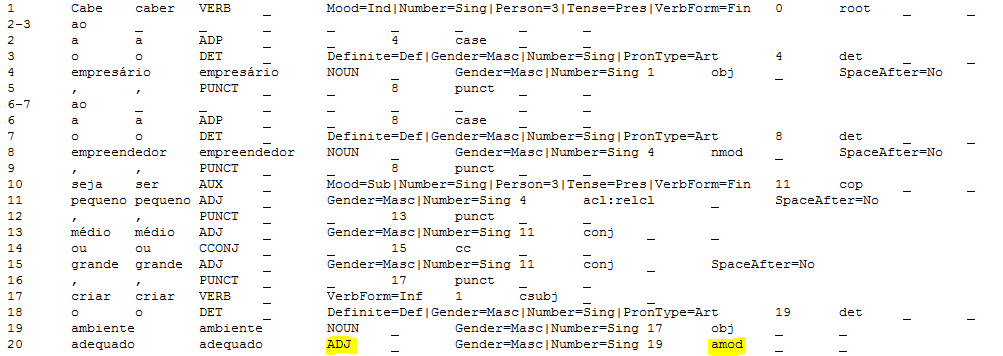
\includegraphics[width=\textwidth,height=\textheight,keepaspectratio]{imagesDrive/image11.png}
			\caption{Cabe ao empresário, ao empreendedor, seja pequeno, médio ou grande, criar o ambiente \emph{adequado} para a valorização de um recurso humano com essas qualificações}
			\label{fig:partadj1}
		\end{figure}{}		
		
		\begin{figure}[H]
			\centering
			\vspace{.8cm}
			\begin{dependency}
				\begin{deptext}
					DET\& NOUN\& ADP\& NOUN\& ADJ\& VERB\& ADP\& NOUN \\
					A\& ideia\& de\& cinema\& engajado\& está\& por\& baixo \\
					o\& ideia\& de\& cinema\& engajado\& estar\& por\& baixo \\
				\end{deptext}
				
				\depedge{2}{1}{det}
				\depedge{6}{2}{nsubj}
				\depedge{4}{3}{case}
				\depedge{2}{4}{nmod}
				\depedge{4}{5}{amod}
				\deproot{6}{root}
				\depedge{8}{7}{case}
				\depedge{6}{8}{obl}
			\end{dependency}
			\caption{A ideia de cinema \emph{engajado} está por baixo}
			\label{fig:partadj2}
		\end{figure}

		\item Formas participiais que estejam em coordenação com outros adjetivos.

		\fullref{fig:partadj3}

		\fullref{fig:partadj4}

		\begin{figure}[H]
			\centering
			\vspace{.8cm}
			\begin{dependency}
				\begin{deptext}
					DET\& NOUN\& ADJ\& CC\& ADV\& ADJ\\
					Este\& futebol\& automatizado\& e\& excessivamente\& defensivo\\
					este\& futebol\& automatizado\& e\& excessivamente\& defensivo\\
				\end{deptext}
				
				\depedge{2}{1}{det}
				\deproot{2}{root}
				\depedge{2}{3}{amod}
				\depedge{6}{4}{cc}
				\depedge{6}{5}{advmod}
				\depedge{3}{6}{conj}

			\end{dependency}
			\caption{Este futebol \emph{automatizado} e excessivamente defensivo}
			\label{fig:partadj3}
		\end{figure}

		\begin{figure}[H]
			\centering
			\vspace{.8cm}
			\begin{dependency}
				\begin{deptext}
					AUX \& DET \& NOUN \& ADV \& ADJ \& PUNCT \& ADV \& ADJ \& CC \& ADV \& ADJ\\
					Foi \& uma \& decisão \& muito \& ponderada \& , \& muito \& difícil \& e \& muito \& amadurecida\\
					ser \& um \& decisão \& muito \& ponderado \& , \& muito \& difícil \& e \& muito \& amadurecido\\
				\end{deptext}
				\depedge{3}{1}{cop}
				\depedge{3}{2}{det}
				\deproot{3}{root}
				\depedge{5}{4}{advmod}
				\depedge{3}{5}{amod}
				\depedge{8}{6}{punct}
				\depedge{8}{7}{advmod}
				\depedge{3}{8}{conj}
				\depedge{11}{9}{cc}
				\depedge{11}{10}{advmod}
				\depedge{3}{11}{conj}
				
			\end{dependency}
			\caption{Foi uma decisão muito \emph{ponderada}, muito difícil e muito amadurecida}
			\label{fig:partadj4}
		\end{figure}

    	\end{enumerate}{}

	\subsection{Formas participiais que são verbo}

	No processo de anotação do Bosque-UD, anotamos como \emph{VERB} (deprel \emph{acl}):

		\begin{enumerate}
		\item Construções em que se pode incluir um agente da passiva sem prejudicar o sentido da frase.
		
		\fullref{fig:partverb1}

		\fullref{fig:partverb2}

			\begin{figure}[H]
			\centering
			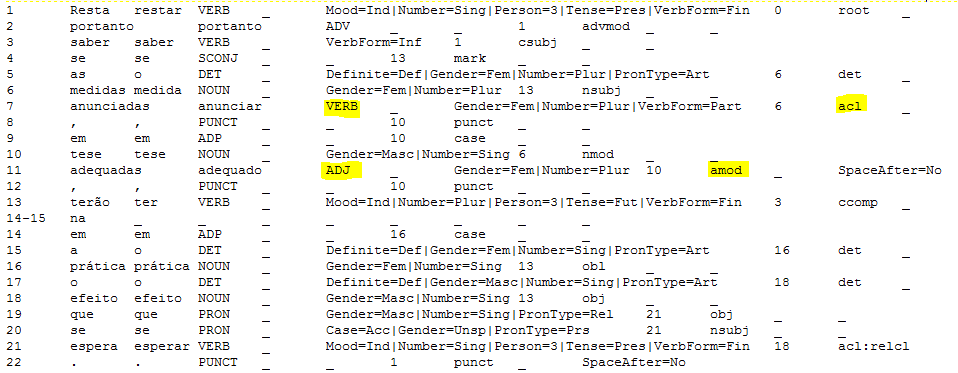
\includegraphics[width=\textwidth,height=\textheight,keepaspectratio]{imagesDrive/image65.png}
			\caption{Resta portanto saber se as medidas \emph{anunciadas}, em tese adequadas, terão na prática o efeito que se espera.}
			\label{fig:partverb1}
		\end{figure}{}		

			\begin{figure}[H]
			\centering
			\vspace{.8cm}
			\begin{dependency}
				\begin{deptext}
					DET \& NOUN \& VERB \& AUX \& NOUN \& ADJ \& CC \& NOUN \& ADP \& NOUN\\
					Os \& serviços \& procurados \& são \& correio \& eletrônico \& e \& transferência \& de \& arquivos\\
					o \& serviço \& procurar \& ser \& correio \& eletrônico \& e \& transferência \& de \& arquivo\\
				\end{deptext}
				\depedge{2}{1}{det}
				\depedge{5}{2}{nsubj}
				\depedge{2}{3}{acl}
				\depedge{5}{4}{cop}
				\deproot{5}{root}
				\depedge{5}{6}{amod}
				\depedge{8}{7}{cc}
				\depedge{5}{8}{conj}
				\depedge{10}{9}{case}
				\depedge{8}{10}{nmod}
				
			\end{dependency}
			\caption{Os serviços \emph{procurados} são correio eletrônico e transferência de arquivos}
			\label{fig:partverb2}
		\end{figure}		
			
		\end{enumerate}

	\subsection{Casos difíceis das formas participiais}

		Como, frequentemente, a decisão será arbitrária, havendo bons argumentos para a leitura verbal e a leitura nominal, listamos aqui as decisões tomadas:

		\begin{enumerate}
		\item Os seguintes casos foram anotados como adjetivo:

		\fullref{fig:partDIF1}

		\fullref{fig:partDIF6}

		\fullref{fig:partDIF7}\newline

		\begin{figure}[H]
			\centering
			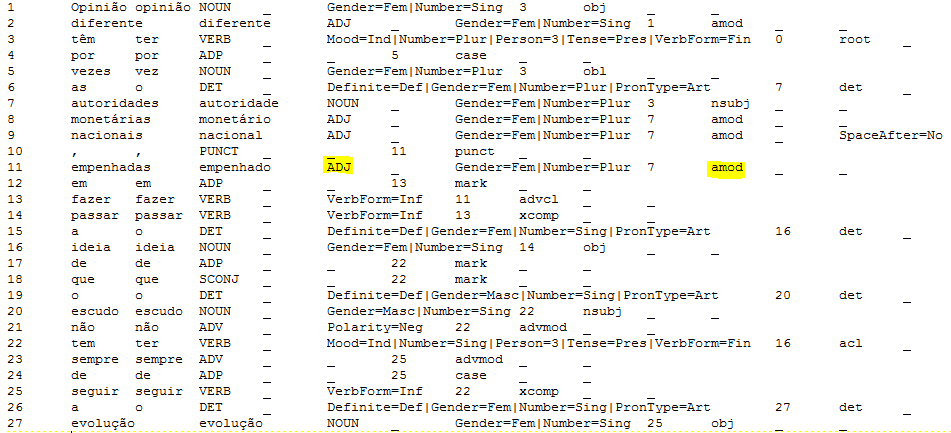
\includegraphics[width=\textwidth,height=\textheight,keepaspectratio]{imagesDrive/image49.png}
			\caption{Opinião diferente têm por vezes as autoridades monetárias nacionais, \emph{empenhadas} em fazer passar a ideia de que o escudo não tem sempre de seguir a evolução da moeda espanhola.}	
			\label{fig:partDIF1}
		\end{figure}	

		\begin{figure}[H]
				\centering
				\vspace{.8cm}
				\begin{dependency}
					\begin{deptext}
						PROPN\& PUNCT\& ADJ\& PUNCT\& VERB\& NOUN\& ADP\& DET\& NOUN\\
						Joilson\& ,\& casado\& ,\& pedia\& informações\& sobre\& o\& abrigo\\
						Joilson\& ,\& casado\& ,\& pedir\& informação\& sobre\& o\& abrigo\\
					\end{deptext}
					
					\depedge{5}{1}{nsubj}
					\depedge{3}{2}{punct}
					\depedge{1}{3}{amod}
					\depedge{3}{4}{punct}
					\deproot{5}{root}
					\depedge{5}{6}{obj}
					\depedge{9}{7}{case}
					\depedge{9}{8}{det}
					\depedge{6}{9}{nmod}
				\end{dependency}
				\caption{Joilson, \emph{casado}, pedia informações sobre o abrigo}
				\label{fig:partDIF6}
			\end{figure}

			\begin{figure}[H]
				\centering
				\vspace{.8cm}
				\begin{dependency}
					\begin{deptext}
						DET\& NOUN\& ADP\& NOUN\& ADJ\\
						O\& procurador\& de\& Justiça\& aposentado\\
						o\& procurador\& de\& justiça\& aposentado\\
					\end{deptext}
					
					\depedge{2}{1}{det}
					\deproot{2}{root}
					\depedge{4}{3}{case}
					\depedge{2}{4}{nmod}
					\depedge{4}{5}{amod}
				\end{dependency}
				\caption{O procurador de Justiça \emph{aposentado}}
				\label{fig:partDIF7}
			\end{figure}

		A presença do \say{mais} pode auxiliar a análise como um adjetivo, ainda que esse critério nem sempre seja definitivo ou preciso. Exemplos:

		\fullref{fig:partDIF2}

		\fullref{fig:partDIF3}

		No exemplo encontrado na \fullref{fig:partDIF3}, temos um caso de \emph{ADJ}/\emph{acl} e não de \emph{ADJ}/\emph{amod}. Aqui, \say{cotado} é o predicativo do sujeito de uma oração predicativa na ordem invertida: \say{O brasileiro Raul Boesel é o mais cotado na bolsa de apostas}. Como o verbo de ligação nunca é o núcleo da oração, o predicativo recebe a etiqueta de \emph{root}. Anotação similar se encontra na \fullref{fig:partDIF9}.

		Em frases como a \fullref{fig:partDIF4}, \say{tão} funciona como \say{mais}. Além disso, há o critério da coordenação.

		\begin{figure}[H]
				\centering
				\vspace{.8cm}
				\begin{dependency}
					\begin{deptext}
						VERB \& ADJ\\
						Chegou \& atrasado\\
						chegar \& atrasado\\
					\end{deptext}
					
					\deproot{1}{root}
					\depedge{1}{2}{acl}
				\end{dependency}
				\caption{Chegou \emph{atrasado}}
				\label{fig:partDIF9}
			\end{figure}

		\begin{figure}[H]
				\centering
				\vspace{.8cm}
				\begin{dependency}
					\begin{deptext}
						VERB\& DET\& NOUN\& ADP\& DET\& NOUN\& ADV\& ADJ\\
						Divulgou\& as\& acusações\& sem\& uma\& checagem\& mais\& aprofundada\\
						divulgar\& o\& acusação\& sem\& um\& checagem\& mais\& aprofundado\\
					\end{deptext}
					
					\deproot{1}{root}
					\depedge{3}{2}{det}
					\depedge{1}{3}{obj}
					\depedge{6}{4}{case}
					\depedge{6}{5}{det}
					\depedge{1}{6}{obl}
					\depedge{8}{7}{advmod}
					\depedge{6}{8}{amod}
				\end{dependency}
				\caption{Divulgou as acusações sem uma checagem mais \emph{aprofundada}}
				\label{fig:partDIF2}
			\end{figure}

			\begin{figure}[H]
			\centering
			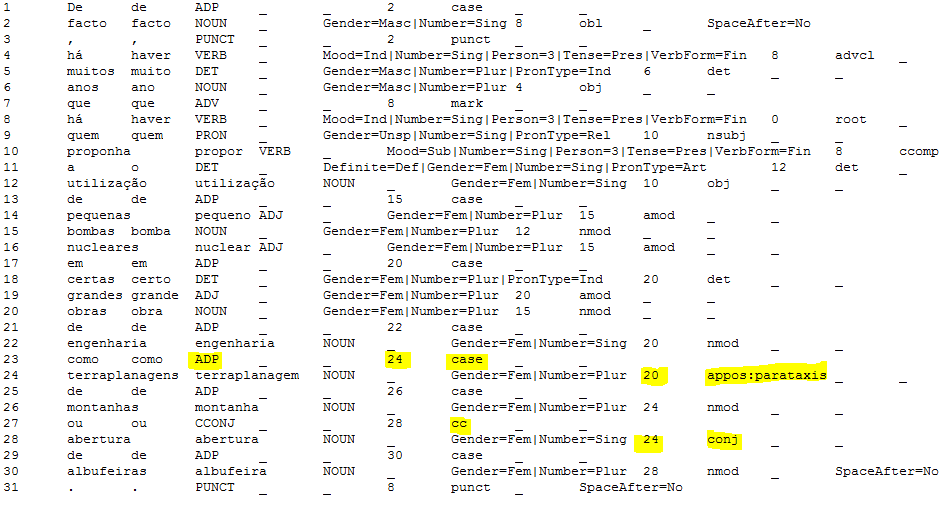
\includegraphics[width=\textwidth,height=\textheight,keepaspectratio]{imagesDrive/image19.png}
			\caption{O mais \emph{cotado} na bolsa de apostas é o brasileiro Raul Boesel, que ontem não consegui terminar a corrida em Detroit}	
			\label{fig:partDIF3}
		\end{figure}
			
			\begin{figure}[H]
			\centering
			\vspace{.8cm}
			\begin{dependency}
				\begin{deptext}
					DET\& NOUN\& ADV\& ADJ\& CC\& ADJ\\
					Um\& coletivo\& tão\& alargado\& e\& dispersivo\\
					um\& coletivo\& tão\& alargado\& e\& dispersivo\\
				\end{deptext}
				
				\depedge{2}{1}{det}
				\deproot{2}{root}
				\depedge{4}{3}{advmod}
				\depedge{2}{4}{amod}
				\depedge{6}{5}{cc}
				\depedge{4}{6}{conj}

			\end{dependency}
			\caption{Um coletivo tão \emph{alargado} e dispersivo}
			\label{fig:partDIF4}
		\end{figure}

		\item Os seguintes casos foram analisados como verbo:

		\fullref{fig:partDIF5}

		\fullref{fig:partDIF8}

		\begin{figure}[H]
			\centering
			\vspace{.8cm}
			\begin{dependency}
				\begin{deptext}
					DET\& NOUN\& PUNCT\& VERB\& ADP\& DET\& NOUN\& PUNCT\& VERB\\
					O\& técnico\& ,\& irritado\& com\& sua\& atuação\& ,\& reclamou\\
					o\& técnico\& ,\& irritar\& com\& seu\& atuação\& ,\& reclamar\\
				\end{deptext}
				
				\depedge{2}{1}{det}
				\depedge{9}{2}{nsubj}
				\depedge{4}{3}{punct}
				\depedge{2}{4}{acl}
				\depedge{7}{5}{case}
				\depedge{7}{6}{det}
				\depedge{4}{7}{obl}
				\depedge{4}{8}{punct}
				\deproot{9}{root}
			\end{dependency}
			\caption{O técnico, \emph{irritado} com sua atuação, reclamou}
			\label{fig:partDIF5}
		\end{figure}

		\begin{figure}[H]
		    \centering
		    \vspace{.8cm}
		    \begin{dependency}
			    \begin{deptext}
			    VERB \& NOUN \& VERB \& SCONJ \& VERB \& NOUN \& ADJ\\
			    Utilizaram \& bactérias \& conhecidas \& por \& devorarem \& material \& orgânico\\
			    utilizar \& bactéria \& conhecer \& por \& devorar \& material \& orgânico\\
			    \end{deptext}
			    \deproot{1}{root}
			    \depedge{1}{2}{obj}
			    \depedge{2}{3}{acl}
			    \depedge{5}{4}{mark}
			    \depedge{3}{5}{xcomp}
			    \depedge{5}{6}{obj}
			    \depedge{6}{9}{amod}
		    \end{dependency}
		    \caption{Utilizaram bactérias conhecidas por devorarem material orgânico}
		    \label{fig:partDIF8}
		\end{figure}

		\item Há casos em que a palavra pode ser anotada como verbo ou adjetivo, dependendo do contexto. Alguns exemplos são \say{passado/a}, \say{elevado/a} e \say{disposto/a}.

		\fullref{fig:passado1}

		\fullref{fig:passado2}\newline

		\fullref{fig:elevado1}

		\fullref{fig:elevado2}\newline

		\fullref{fig:disposto1}

		\fullref{fig:disposto2}

		\begin{figure}[H]
			\centering
			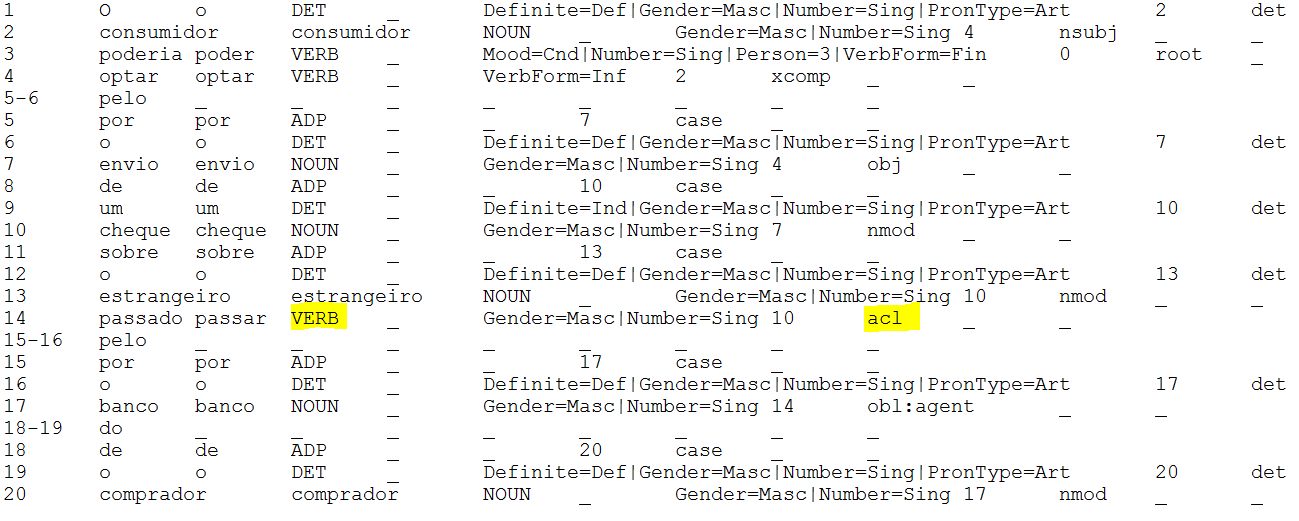
\includegraphics[width=\textwidth,height=\textheight,keepaspectratio]{imagesDrive/passado1.png}
			\caption{O consumidor poderia optar pelo envio de um cheque sobre o estrangeiro \emph{passado} pelo banco do comprador}	
			\label{fig:passado1}
		\end{figure}

		\begin{figure}[H]
			\centering
			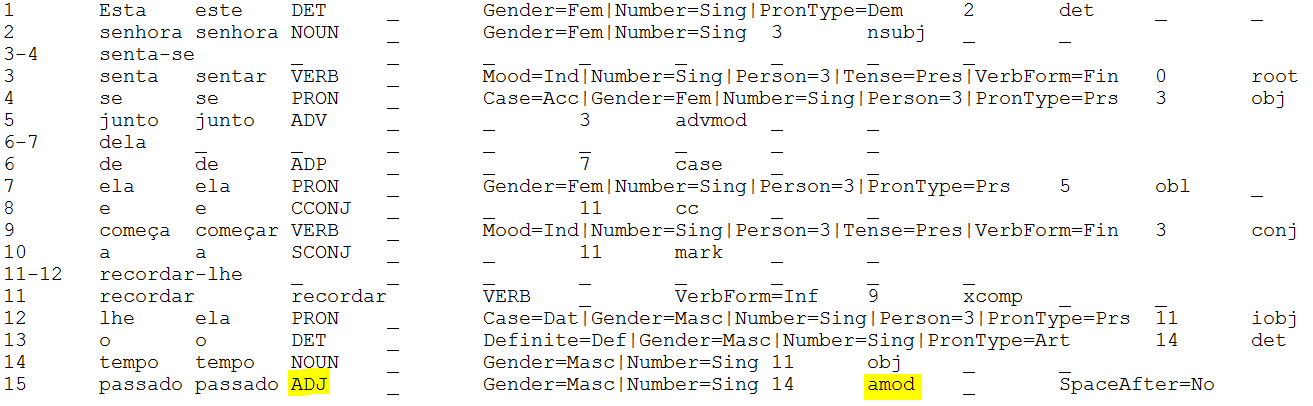
\includegraphics[width=\textwidth,height=\textheight,keepaspectratio]{imagesDrive/passado2.png}
			\caption{Esta senhora senta-se junto dela e começa a recordar-lhe o tempo \emph{passado}}	
			\label{fig:passado2}
		\end{figure}

		\begin{figure}[H]
			\centering
			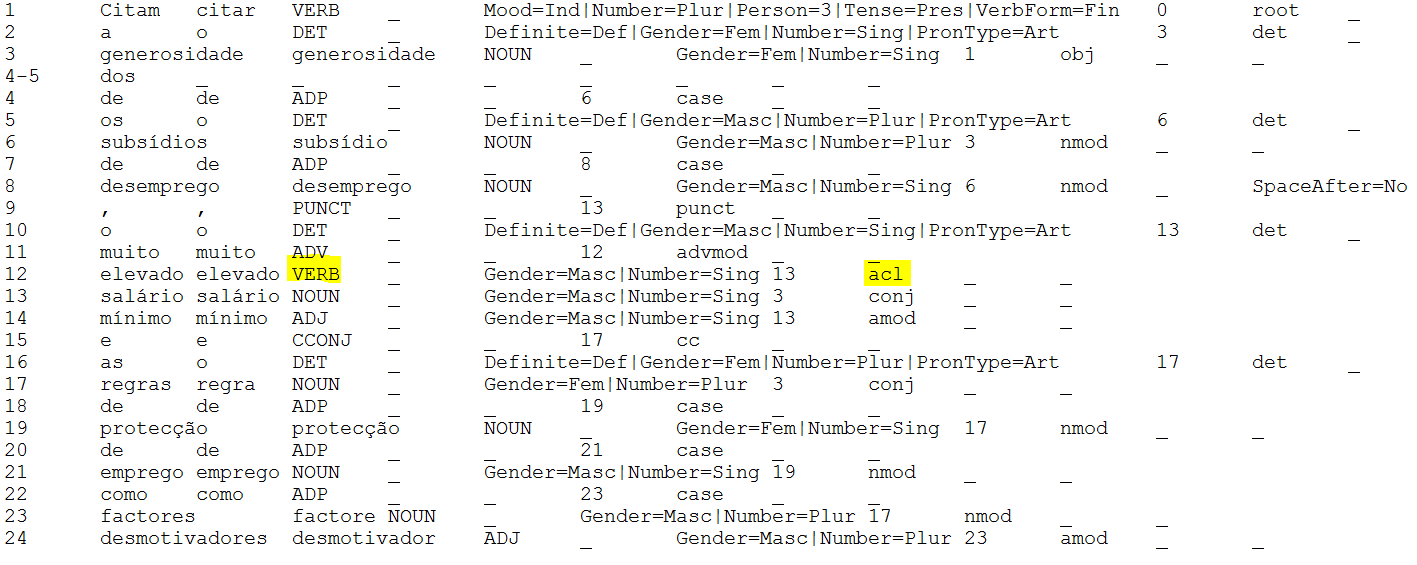
\includegraphics[width=\textwidth,height=\textheight,keepaspectratio]{imagesDrive/elevado1.png}
			\caption{Citam a generosidade dos subsídios de desemprego, o muito \emph{elevado} salário mínimo e as regras de protecção de emprego como factores desmotivadores da criação de postos de trabalho}	
			\label{fig:elevado1}
		\end{figure}

		\begin{figure}[H]
			\centering
			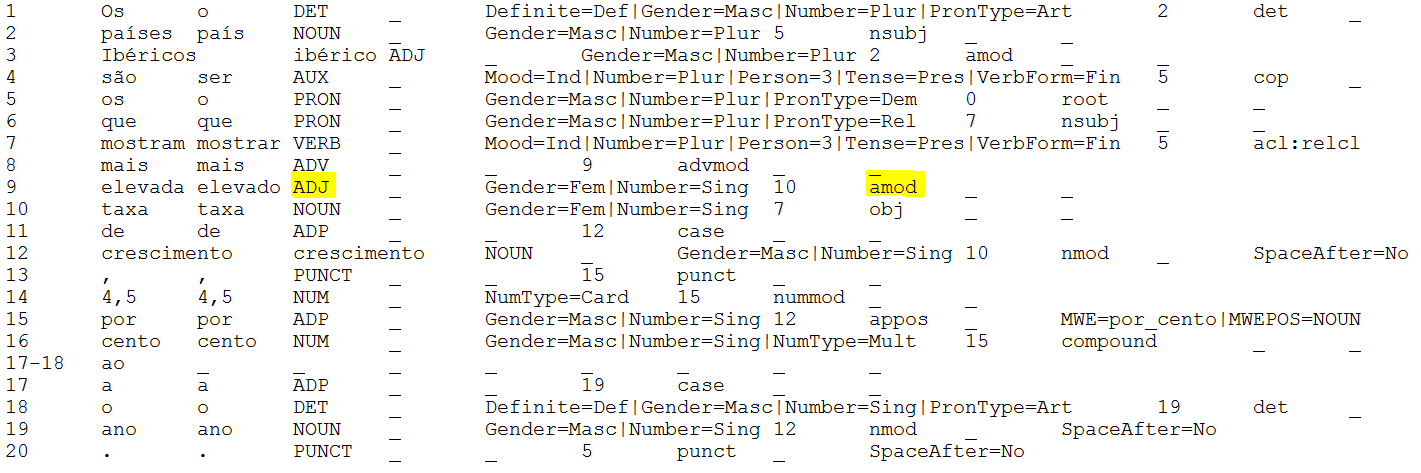
\includegraphics[width=\textwidth,height=\textheight,keepaspectratio]{imagesDrive/elevado2.png}
			\caption{Os países Ibéricos são os que mostram mais \emph{elevada} taxa de crescimento, 4,5 por cento ao ano}	
			\label{fig:elevado2}
		\end{figure}

		\begin{figure}[H]
			\centering
			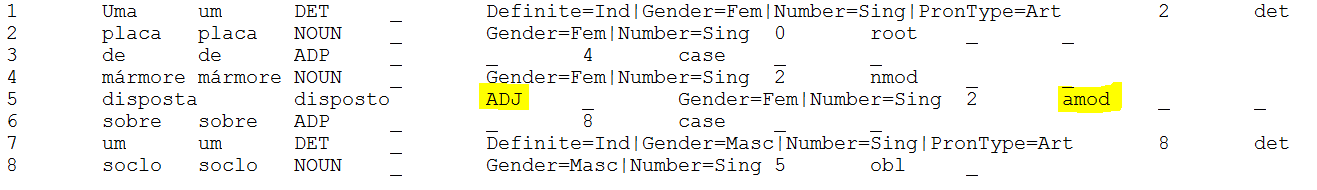
\includegraphics[width=\textwidth,height=\textheight,keepaspectratio]{imagesDrive/disposto1.png}
			\caption{Uma placa de mármore \emph{disposta} sobre um soclo}	
			\label{fig:disposto1}
		\end{figure}

		\begin{figure}[H]
			\centering
			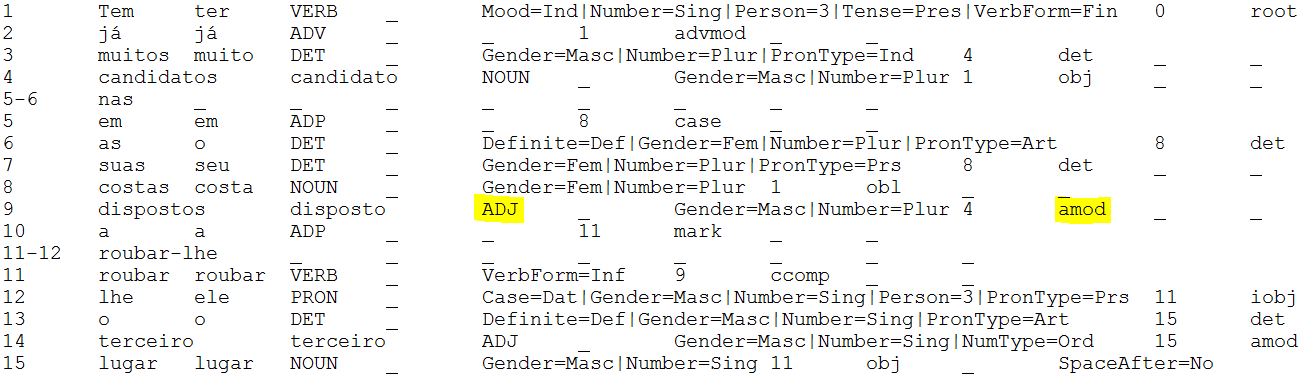
\includegraphics[width=\textwidth,height=\textheight,keepaspectratio]{imagesDrive/disposto2.png}
			\caption{Tem já muitos candidatos nas suas costas \emph{dispostos} a roubar-lhe o terceiro lugar}	
			\label{fig:disposto2}
		\end{figure}

	\end{enumerate}

	\subsection{Formas participiais que não são nem adjetivo nem verbo}

		Há ainda os casos em que as formas participiais serão coisa.

		Por exemplo, em \fullref{dep:partdet}. Neste caso, \say{determinado} é equivalente a \say{certo}, ou \say{algum}. Por isso, será analisado como \emph{DET} (com \emph{PronType=Ind} em suas features e a deprel será \emph{det})
		
		Em \fullref{dep:partnoun}, analisamos \say{aposentados} e \say{casados} como \emph{NOUN}.

		\begin{figure}[H]
			\centering
			\vspace{.8cm}
			\begin{dependency}
				\begin{deptext}
					NOUN \& CCONJ \& NOUN \& ADP \& NOUN \& ADJ \& ADP \& DET \& NOUN \\
					ovos \& e \& larvas \& de \& peixes \& presentes \& em \& determinado \& local \\
					ovo \& e \& larva \& de \& peixe \& presente \& em \& determinado \& local \\
					 \&  \&  \&  \&  \&  \&  \& PronType=Ind \&  \& \\
				\end{deptext}
				\depedge{3}{2}{cc}
				\depedge{1}{3}{conj}
				\depedge{5}{4}{case}
				\depedge{1}{5}{nmod}
				\depedge{1}{6}{acl}
				\depedge{9}{6}{obl}
				\depedge{9}{8}{det}
				\depedge{9}{7}{case}
				\deproot{1}{root}
			\end{dependency}
			\caption{ovos e larvas de peixes possivelmente \emph{presentes} em determinado local}
			\label{dep:partdet}
		\end{figure}

		\begin{figure}[H]
			\centering
			\vspace{.8cm}
			\begin{dependency}
				\begin{deptext}
					DET \& NOUN \& PUNCT \& CCONJ \& DET \& NOUN \& PUNCT \& AUX \& ADJ \\
					os \& aposentados \& ( \& e \& os \& casados \& ) \& são \& maioria \\
					o \& aposentado \& ( \& e \& o \& casado \& ) \& ser \& maioria \\
				\end{deptext}
				\depedge{2}{1}{det}
				\depedge{6}{3}{punct}
				\depedge{6}{4}{cc}
				\depedge{6}{5}{det}
				\depedge{6}{7}{punct}
				\depedge{9}{8}{cop}
				\depedge{9}{2}{nsubj}
				\depedge{2}{6}{conj}
				\deproot{2}{root}
			\end{dependency}
			\caption{os \emph{aposentados} (e os \emph{casados}) são maioria}
			\label{dep:partnoun}
		\end{figure}


\section{Numerais}\label{sec:numerais}

	Numerais \emph{cardinais} (\say{360}) e \emph{fracionários} (\fullref{dep:numfrac}) e algarismos romanos devem ser anotados como \emph{NUM}, sejam por extenso ou em algarismos.

	Numerais \emph{multiplicativos} (\say{dobro}, \say{triplo}, etc.), por outro lado, devem ser anotados como \emph{NOUN}. Trata-se de uma abordagem diferente da proposta pelas diretivas oficiais do projeto Universal Dependencies (a consulta foi realizada dia 5 de março de 2020), uma vez que, nos exemplos propostos por eles, em inglês, \say{once} e \say{twice} funcionam como advérbios, modificando o verbo, enquanto que no português estas palavras não existem, e os numerais multiplicativos, como \say{dobro}, modificam um nome como adjunto adnominal (ver \fullref{sec:adjuntoadnominal}).
	
	Numerais coletivos (como \say{dezenas}, \say{centenas}, \say{milhares}, etc.), no corpus Bosque-UD, podem estar anotados de duas formas diferentes, conforme o contexto: como \emph{NUM}, caso seja um número exato (\say{duas centenas}, \say{dois bilhões}), ou como \emph{NOUN}, quando é indefinido (\say{centenas de pessoas}).
	
	Numerais ordinais devem ser anotados como de upos \textit{ADJ} (\fullref{sec:adjounum}).
	
	Ver também: \fullref{sec:numeroscompostos}
	
	\begin{figure}[H]
		\centering
		\vspace{.8cm}
		\begin{dependency}
			\begin{deptext}
				NUM \& NOUN \& CCONJ \& NUM \\
				2 \& casas \& e \& meia \\
				2 \& casa \& e \& meio \\
				NumType=Card \& \& \& NumType=Frac \\
			\end{deptext}
			\depedge{2}{1}{nummod}
			\depedge{1}{3}{flat}
			\depedge{1}{4}{flat}
			\deproot{2}{root}
		\end{dependency}
		\caption{\textit{2 casas e meia}}
		\label{dep:numfrac}
	\end{figure}

	\subsection{Números compostos}\label{sec:numeroscompostos}
	
		Números compostos podem conter upos \emph{NUM} e \emph{CCONJ}. 
		
		A maneira de garantir que números compostos são \emph{um número}, isto é, que \say{106} é o mesmo que \say{cento e seis}, uma unidade, é pela sintaxe: números compostos estarão relacionados pela deprel \say{flat}, e todos serão filhos da primeira palavra do número. Ou seja, em \say{cento e quinze mil}, \say{cento} é o head (núcleo) e \say{e}, \say{quinze}, \say{mil} apontam para \say{cento} como \emph{flat}.

		Quando o número composto modifica um substantivo (\fullref{dep:trintaesete}), o primeiro número deve se subordinar ao substantivo como de deprel \emph{nummod}.

		Quando há um sintagma preposicionado (\fullref{dep:montantede}), a relação se inverte: o primeiro número do número composto será o head (\say{1300}), e o substantivo (\say{dólares}), \emph{nmod} do número.
		
		\begin{figure}[H]
			\centering
			\vspace{.8cm}
			\begin{dependency}
				\begin{deptext}
					NUM \& CCONJ \& NUM \& NOUN \\
					Trinta \& e \& sete \& casas \\
					trinta \& e \& sete \& casa \\
					NumType=Card \& \& NumType=Card \& \\
				\end{deptext}
				\depedge{1}{2}{flat}
				\depedge{1}{3}{flat}
				\depedge{4}{1}{nummod}
				\deproot{4}{root}
			\end{dependency}
			\caption{\textit{Trinta e sete}}
			\label{dep:trintaesete}
		\end{figure}
	
		\begin{figure}[H]
			\centering
			\vspace{.8cm}
			\begin{dependency}
				\begin{deptext}
					NOUN \& ADP \& NUM \& NUM \& ADP \& NOUN \\
					Montante \& de \& 1300 \& milhões \& de \& dólares \\
					montante \& de \& 1300 \& milhão \& de \& dólar \\
					\& \& NumType=Card \& NumType=Card \\
				\end{deptext}
				\depedge{3}{2}{case}
				\depedge{3}{4}{flat}
				\deproot{1}{root}
				\depedge{1}{3}{nummod}
				\depedge{6}{5}{case}
				\depedge{3}{6}{nmod}
			\end{dependency}
			\caption{Montante de \textit{1300 milhões de dólares}}
			\label{dep:montantede}
		\end{figure}
	
	\subsection{\textit{R\$ 50}: quem é o pai?}\label{sec:rs50}
	
		Quando há a inserção de símbolos como \fullref{dep:rs50}, \fullref{dep:us50} ou \fullref{dep:50porcento}, o símbolo deve ser o head.

		No caso de números coletivos (\fullref{dep:2centenas}), o primeiro número será o head, e o coletivo será \emph{flat}. Ver: \fullref{sec:numeroscompostos}.
		
		\begin{figure}[H]
			\centering
			\vspace{.8cm}
			\begin{dependency}
				\begin{deptext}
					SYM \& NUM \\
					R\$ \& 50 \\
					R\$ \& 50 \\
					\& NumType=Card \\
				\end{deptext}
				\depedge{1}{2}{nummod}
				\deproot{1}{root}
			\end{dependency}
			\caption{\textit{R\$ 50}}
			\label{dep:rs50}
		\end{figure}
	
		\begin{figure}[H]
			\centering
			\vspace{.8cm}
			\begin{dependency}
				\begin{deptext}
					SYM \& NUM \\
					U\$ \& 50 \\
					U\$ \& 50 \\
					\& NumType=Card \\
				\end{deptext}
				\depedge{1}{2}{nummod}
				\deproot{1}{root}
			\end{dependency}
			\caption{\textit{U\$ 50}}
			\label{dep:us50}
		\end{figure}
	
		\begin{figure}[H]
			\centering
			\vspace{.8cm}
			\begin{dependency}
				\begin{deptext}
					NUM \& SYM \\
					50 \& \% \\
					50 \& \% \\
					NumType=Card \& \\
				\end{deptext}
				\depedge{2}{1}{nummod}
				\deproot{2}{root}
			\end{dependency}
			\caption{\textit{50\%}}
			\label{dep:50porcento}
		\end{figure}
	
		\begin{figure}[H]
			\centering
			\vspace{.8cm}
			\begin{dependency}
				\begin{deptext}
					NUM \& NUM \\
					2 \& centenas \\
					2 \& centena \\
					NumType=Card \& NumType=Card \\
				\end{deptext}
				\depedge{1}{2}{flat}
				\deproot{1}{root}
			\end{dependency}
			\caption{\textit{2 centenas}}
			\label{dep:2centenas}
		\end{figure}
	
	\subsection{\textit{50\% das pessoas}: quem é o pai?}\label{sec:50porcentodaspessoas}
	
		Sempre que houver sintagma preposicionado, o sintagma anterior será o head, como em \fullref{dep:50porcentodaspessoas} (onde o símbolo é o head, segundo \fullref{sec:rs50}), e \fullref{dep:montantede}.
	
		\begin{figure}[H]
			\centering
			\vspace{.8cm}
			\begin{dependency}
				\begin{deptext}
					NUM \& SYM \& ADP \& DET \& NOUN \\
					50 \& \% \& de \& as \& pessoas \\
					50 \& \% \& de \& as \& pessoa \\
					NumType=Card \\
				\end{deptext}
				\depedge{2}{1}{nummod}
				\deproot{2}{root}
				\depedge{5}{3}{case}
				\depedge{5}{4}{det}
				\depedge{2}{5}{nmod}
			\end{dependency}
			\caption{\textit{50\% das pessoas}}
			\label{dep:50porcentodaspessoas}
		\end{figure}
	
	\subsection{\textit{Primeiro} lugar: adjetivo ou numeral?}\label{sec:adjounum}
	
		Numerais ordinais escritos por extenso ou em algarismos devem ser anotados como de upos \emph{ADJ}, e recebem a feature \emph{NumType=Ord}, como na \fullref{dep:primeiratentativa}.
		
		\begin{figure}[H]
		    \centering
		    \vspace{.8cm}
		    \begin{dependency}
		    \begin{deptext}
		    ADJ \& NOUN \\
		    Primeira \& tentativa \\
		    primeiro \& tentativa \\
		    NumType=Ord \& \\
		    \end{deptext}
		    \depedge{2}{1}{amod}
		    \deproot{2}{root}
		    \end{dependency}
		    \caption{\textit{Primeira tentativa}}\label{dep:primeiratentativa}
		\end{figure}

	\subsection{\emph{um}: numeral, pronome ou artigo?}\label{sec:numeralpronomeouartigo}

		Em português, a palavra \say{um} pode ser classificada de diversas maneiras. Definimos situações em que a sua leitura preferencial será numeral, artigo ou pronome.

		\say{um} será numeral em todos os casos em que estiver quantificando, de maneira clara, um nome, garantindo-se que não é possível, de maneira alguma, a leitura de indeterminação, já que o papel do numeral é, justamente, \textbf{determinar} quantidade. É o caso de \fullref{dep:umnumeral1} e \fullref{dep:umnumeral2}.

		\say{um} será artigo indefinido em todos os casos em que estiver modificando um nome e a leitura de indeterminação for possível. É o caso de \fullref{dep:umartigo1} e \fullref{dep:umartigo2}.

		\say{um} será pronome indefinido em todos os casos em que estiver substituindo um nome. É o caso de \fullref{dep:umpronome1} e \fullref{dep:umpronome2}.

		\begin{figure}[H]
		        \centering
		        \vspace{.8cm}
		        \begin{dependency}
		                \begin{deptext}
		                        VERB \& ADV \& NUM \& NOUN \& ADP \& NOUN \& ADP \& DET \& NOUN \\
		                        pediu \& mais \& um \& dia \& de \& folga \& a \& o \& treinador \\
		                        pedir \& mais \& um \& dia \& de \& folga \& a \& o \& treinador \\
					 \&  \& NumType=Card \&  \&  \&  \& \& \& \\
		                \end{deptext}
		                \deproot{1}{root}
		                \depedge{3}{2}{advmod}
		                \depedge{4}{3}{nummod}
		                \depedge{1}{4}{obj}
		                \depedge{6}{5}{case}
		                \depedge{4}{6}{nmod}
		                \depedge{9}{7}{case}
		                \depedge{9}{8}{det}
		                \depedge{1}{9}{iobj}
		        \end{dependency}
		        \caption{pediu mais \emph{um} dia de folga a o treinador}
		        \label{dep:umnumeral1}
		\end{figure}

		\begin{figure}[H]
		        \centering
		        \vspace{.8cm}
		        \begin{dependency}
		                \begin{deptext}
		                        AUX \& ADJ \& ADP \& DET \& PROPN \& ADP \& ADV \& NUM \& NOUN \\
		                        São \& vistos \& por \& a \& CPI \& como \& mais \& um \& indício \\
		                        ser \& ver \& por \& o \& CPI \& como \& mais \& um \& indício \\
		                         \&  \&  \&  \&  \&  \&  \& NumType=Card \&  \& \\
		                \end{deptext}
		                \depedge{2}{1}{aux}
		                \deproot{2}{root}
		                \depedge{5}{3}{case}
		                \depedge{5}{4}{det}
		                \depedge{2}{5}{obl}
		                \depedge{9}{6}{case}
		                \depedge{8}{7}{advmod}
		                \depedge{9}{8}{nummod}
		                \depedge{2}{9}{xcomp}
		        \end{dependency}
		        \caption{São vistos por a CPI como mais \emph{um} indício}
		        \label{dep:umnumeral2}
		\end{figure}

		\begin{figure}[H]
		        \centering
		        \vspace{.8cm}
		        \begin{dependency}
		                \begin{deptext}
		                        DET \& NOUN \& ADP \& DET \& NOUN \& VERB \& DET \& NOUN \& ADJ \\
		                        O \& governo \& de \& o \& Estado \& realizará \& um \& concurso \& público \\
		                        o \& governo \& de \& o \& estado \& realizar \& um \& concurso \& público \\
		                         \&  \&  \&  \&  \&  \& Definite=Ind \&  \&  \\
		                         \&  \&  \&  \&  \&  \& PronType=Art  \&  \&  \\
		                \end{deptext}
		                \depedge{2}{1}{det}
		                \depedge{6}{2}{nsubj}
		                \depedge{5}{3}{case}
		                \depedge{5}{4}{det}
		                \depedge{2}{5}{nmod}
		                \deproot{6}{root}
		                \depedge{8}{7}{det}
		                \depedge{6}{8}{obj}
		                \depedge{8}{9}{amod}
		        \end{dependency}
		        \caption{O governo de o Estado realizará \emph{um} concurso público}
		        \label{dep:umartigo1}
		\end{figure}

		\begin{figure}[H]
		        \centering
		        \vspace{.8cm}
		        \begin{dependency}
		                \begin{deptext}
		                        VERB \& DET \& NOUN \& SCONJ \& PRON \& VERB \\
		                        Encontraram \& um \& discurso \& para \& se \& diferenciar \\
		                        encontrar \& um \& discurso \& para \& se \& diferenciar \\
		                         \& Definite=Ind  \&  \&  \&  \&  \\
		                         \& PronType=Art  \&  \&  \&  \&  \\
		                \end{deptext}
		                \deproot{1}{root}
		                \depedge{3}{2}{det}
		                \depedge{1}{3}{obj}
		                \depedge{6}{4}{mark}
		                \depedge{6}{5}{expl}
		                \depedge{1}{6}{advcl}
		        \end{dependency}
		        \caption{Encontraram \emph{um} discurso para se diferenciar}
		        \label{dep:umartigo2}
		\end{figure}

		\begin{figure}[H]
		        \centering
		        \vspace{.8cm}
		        \begin{dependency}
		                \begin{deptext}
		                        NUM \& NOUN \& ADP \& PRON \& PUNCT \& NUM \& ADP \& PRON \\
		                        quatro \& disparos \& em \& um \& , \& seis \& em \& outro \\
		                        quatro \& disparo \& em \& um \& , \& seis \& em \& outro \\
		                         \&  \&  \& PronType=Ind  \&  \&  \&  \&  \\
		                \end{deptext}
		                \depedge{2}{1}{nummod}
		                \deproot{2}{root}
		                \depedge{4}{3}{case}
		                \depedge{2}{4}{obl}
		                \depedge{6}{5}{punct}
		                \depedge{2}{6}{conj}
		                \depedge{8}{7}{case}
		                \depedge{6}{8}{orphan}
		        \end{dependency}
		        \caption{quatro disparos em \emph{um} , seis em outro}
		        \label{dep:umpronome1}
		\end{figure}

		\begin{figure}[H]
		        \centering
		        \vspace{.8cm}
		        \begin{dependency}
		                \begin{deptext}
		                        VERB \& ADP \& PRON \& ADP \& DET \& NOUN \& ADP \& DET \& NOUN \& ADJ \\
		                        estamos \& perante \& um \& de \& os \& documentos \& de \& o \& art. \& 46º \\
		                        estar \& perante \& um \& de \& o \& documento \& de \& o \& art. \& 46º \\
		                         \&  \& PronType=Ind \&  \&  \&  \&  \&  \&  \&  \\
		                \end{deptext}
		                \deproot{1}{root}
		                \depedge{3}{2}{case}
		                \depedge{1}{3}{obl}
		                \depedge{6}{4}{case}
		                \depedge{6}{5}{det}
		                \depedge{3}{6}{nmod}
		                \depedge{9}{7}{case}
		                \depedge{9}{8}{det}
		                \depedge{6}{9}{nmod}
		                \depedge{9}{10}{amod}
		        \end{dependency}
		        \caption{estamos perante \emph{um} de os documentos de o art. 46º}
		        \label{dep:umpronome2}
		\end{figure}

\section{Artigos, pronomes substantivos e pronomes adjetivos}\label{sec:pronedet}

	Pronomes substantivos são anotados como \textit{PRON} (\fullref{dep:pronsubst}).
	
	Pronomes adjetivos são anotados como de upos \textit{DET}, e recebem deprel \textit{det}, sendo dependentes do token que modificam (\fullref{dep:pronadj}).
	
	Artigos, assim como adjetivos, também são anotados como \textit{DET/det}, como na \fullref{dep:artdet}, e devem receber o valor \emph{PronType=Art} na coluna feats, além de \emph{Definite=[Def, Ind]}.

	E lembramos que \say{cujo/cuja} são os únicos pronomes relativos que são pronomes adjetivos (\emph{DET}), e não substantivos (\emph{PRON}).

	Ver também:

	\fullref{sec:pronint}

	\fullref{sec:prondem}

	\fullref{sec:pronrel}

	\fullref{sec:pronind}

	\fullref{sec:numeralpronomeouartigo}
	
	\begin{figure}[H]
		\centering
		\vspace{.8cm}
		\begin{dependency}
			\begin{deptext}
				ADV \& PRON \& AUX \& ADV \& NOUN \& ADP \& PRON \& PUNCT \\
				Talvez \& isto \& seja \& muito \& barulho \& por \& nada \& . \\
				talvez \& isto \& ser \& muito \& barulho \& por \& nada \& . \\
				\& PronType=Dem \& \& \& \& \& \& \\
			\end{deptext}
			\depedge{5}{1}{advmod}
			\depedge{5}{2}{nsubj}
			\depedge{5}{3}{cop}
			\depedge{5}{4}{advmod}
			\depedge{7}{6}{case}
			\depedge{5}{7}{nmod}
			\depedge{5}{8}{punct}
			\deproot{5}{root}
		\end{dependency}
		\caption{Talvez \textit{isto} seja muito barulho por nada}\label{dep:pronsubst}
	\end{figure}

	\begin{figure}[H]
		\centering
		\vspace{.8cm}
		\begin{dependency}
			\begin{deptext}
				DET \& NOUN \& VERB \& PRON \& DET \& NOUN \& ADJ \& PUNCT \\
				Aquele \& pensamento \& provocou \& me \& um \& arrepio \& delicioso \& . \\
				aquele \& pensamento \& provocar \& eu \& um \& arrepio \& delicioso \& . \\
				PronType=Dem \& \& \& \& \& \& \& \\
			\end{deptext}
			\deproot{3}{root}
			\depedge{2}{1}{det}
			\depedge{3}{2}{nsubj}
			\depedge{3}{4}{iobj}
			\depedge{6}{5}{det}
			\depedge{3}{6}{obj}
			\depedge{6}{7}{amod}
			\depedge{3}{8}{punct}
		\end{dependency}
		\caption{\textit{Aquele} pensamento provocou-me um arrepio delicioso}\label{dep:pronadj}
	\end{figure}

	\begin{figure}[H]
		\centering
		\vspace{.8cm}
		\begin{dependency}
			\begin{deptext}
				AUX \& DET \& NOUN \& ADP \& DET \& NOUN \& ADP \& DET \& NOUN \& PUNCT \\
				Eram \& o \& retrato \& de \& o \& cérebro \& de \& este \& partido \& . \\
				ser \& o \& retrato \& de \& o \& cérebro \& de \& este \& partido \& . \\
				      \& Definite=Def \& \& \& \& \& \& \& \& \\
				      \& PronType=Art \& \& \& \& \& \& \& \& \\
			\end{deptext}
			\depedge{3}{1}{cop}
			\depedge{3}{6}{nmod}
			\depedge{6}{9}{nmod}
			\depedge{3}{2}{det}
			\depedge{6}{4}{case}
			\depedge{6}{5}{det}
			\depedge{9}{7}{case}'
			\depedge{9}{8}{det}
			\depedge{3}{10}{punct}
			\deproot{3}{root}
		\end{dependency}
		\caption{Eram \textit{o} retrato d\textit{o} cérebro deste partido}\label{dep:artdet}
	\end{figure}

	\subsection{Pronomes interrogativos}\label{sec:pronint}

		Pronomes interrogativos, assim como os pronomes substantivos, têm upos \textit{PRON} e recebem a deprel do sintagma (\fullref{dep:pronint}). Não confundir com os advérbios interrogativos (\fullref{sec:adverbiosinterrogativos}), que podem inclusive se tornar conjunções quando introduzindo orações subordinadas \fullref{sec:classesdinamicas}.

		\begin{figure}[H]
			\centering
			\vspace{.8cm}
			\begin{dependency}
				\begin{deptext}
					CCONJ \& VERB \& PRON \& PRON \& ADV \& ADV \& VERB \& PUNCT \\
					E \& sabe \& quem \& eu \& ainda \& não \& vi \& ? \\
					e \& saber \& quem \& eu \& ainda \& não \& ver \& ? \\
					\& \& PronType=Int \& \& \& Polarity=Neg \& \& \\
				\end{deptext}
				\depedge{2}{1}{cc}
				\depedge{7}{3}{obj}
				\depedge{2}{7}{ccomp}
				\depedge{2}{8}{punct}
				\depedge{7}{4}{nsubj}
				\depedge{7}{6}{advmod}
				\depedge{7}{5}{advmod}
				\deproot{2}{root}
			\end{dependency}
			\caption{E sabe \textit{quem} eu ainda não vi?}\label{dep:pronint}
		\end{figure}

	\subsection{Pronomes demonstrativos}\label{sec:prondem}

		Pronomes demonstrativos devem receber a etiqueta \emph{PronType=Dem} na coluna feats.

		Podem ser classificados tanto como pronomes substantivos, quando substituem um substantivo (\fullref{dep:pronsubst}), quanto como pronomes adjetivos (\fullref{dep:pronadj}), quando modificam um substantivo.

	\subsection{Pronomes relativos}\label{sec:pronrel}

		Pronomes relativos devem receber o valor \emph{PronType=Rel} na coluna feats. Recebem a deprel da função sintática que exercem na oração que iniciam.

		\say{Cujo/a} são os únicos pronomes relativos que são pronomes adjetivos (\emph{DET}), e não substantivos.

		\fullref{dep:relque}

		\fullref{dep:relonde}

		\fullref{dep:relcuja}

		\begin{figure}[H]
			\centering
			\vspace{.8cm}
			\begin{dependency}
				\begin{deptext}
					PRON \& PRON \& VERB \& AUX \& DET \& NOUN \& PUNCT \& PUNCT \& VERB \& PUNCT \\
					O \& que \& fizeram \& foi \& um \& absurdo \& » \& , \& disse \& . \\
					o \& que \& fazer \& ser \& um \& absurdo \& » \& , \& dizer \& . \\
 					\& PronType=Rel \& \& \& \& \& \& \& \& \\
				\end{deptext}
				\depedge{9}{6}{parataxis}
				\depedge{3}{2}{det}
				\depedge{1}{3}{acl:relcl}
				\depedge{6}{4}{cop}
				\depedge{6}{5}{det}
				\depedge{6}{7}{punct}
				\depedge{6}{8}{punct}
				\depedge{9}{10}{punct}
				\depedge{6}{1}{nsubj}
				\deproot{9}{root}
			\end{dependency}
			\caption{O \emph{que} fizeram foi um absurdo», disse}\label{dep:relque}
		\end{figure}

		\begin{figure}[H]
			\centering
			\vspace{.8cm}
			\begin{dependency}
				\begin{deptext}
					VERB \& DET \& NOUN \& PRON \& DET \& NOUN \& VERB \& PUNCT \\
					Observou \& os \& lugares \& onde \& essas \& pessoas \& almoçam \& . \\
					observar \& o \& lugar \& onde \& esse \& pessoa \& almoçar \& . \\
					\& \& \& PronType=Rel \& \& \& \& \\
				\end{deptext}
				\depedge{7}{4}{obl}
				\depedge{6}{5}{det}
				\depedge{7}{6}{nsubj}
				\depedge{3}{7}{acl:relcl}
				\depedge{3}{2}{det}
				\depedge{1}{3}{obj}
				\depedge{3}{7}{acl:relcl}
				\depedge{1}{8}{punct}
				\deproot{1}{root}
			\end{dependency}
			\caption{Observou \emph{onde} essas pessoas almoçam}\label{dep:relonde}
		\end{figure}

		\begin{figure}[H]
			\centering
			\vspace{.8cm}
			\begin{dependency}
				\begin{deptext}
					DET \& NOUN \& DET \& NOUN \& VERB \& NOUN \\
					Uma \& galeria \& cuja \& concepção \& permitirá \& intervenções \& . \\
					um \& galeria \& cujo \& concepção \& permitir \& intervenção \& . \\
					\& \& PronType=Rel \& \& \& \\
				\end{deptext}
				\depedge{2}{1}{det}
				\depedge{5}{4}{nsubj}
				\depedge{4}{3}{det}
				\depedge{2}{5}{acl:relcl}
				\depedge{5}{6}{obj}
				\deproot{2}{root}
				\depedge{2}{7}{punct}
			\end{dependency}
			\caption{Uma galeria \emph{cuja} concepção permitirá intervenções no subsolo}\label{dep:relcuja}
		\end{figure}


	\subsection{Pronomes indefinidos}\label{sec:pronind}

		Pronomes indefinidos devem receber o valor \emph{PronType=Ind} na coluna feats, e podem ser pronomes substantivos (upos \emp{PRON}), como na \fullref{dep:pronindsubst}, ou adjetivos (upos \emp{DET}), como na \fullref{dep:pronindadj}.

		\begin{figure}[H]
			\centering
			\vspace{.8cm}
			\begin{dependency}
				\begin{deptext}
					PRON \& VERB \& DET \& NOUN \\
					Ninguém \& força \& sua \& escalação \\
					ninguém \& forçar \& seu \& escalação \\
					PronType=Ind \& \& \& \\
				\end{deptext}
				\depedge{4}{3}{det}
				\depedge{2}{4}{obj}
				\depedge{2}{1}{nsubj}
				\deproot{2}{root}
			\end{dependency}
			\caption{\emph{Ninguém} força sua escalação}\label{dep:pronindsubst}
		\end{figure}

		\begin{figure}[H]
					\centering
					\vspace{.8cm}
					\begin{dependency}
						\begin{deptext}
								DET \& NOUN \& ADJ \& ADV \& PRON \& VERB \& SCONJ \& VERB \& DET \& DET \& NOUN \\
								A \& comissão \& técnica \& não \& se \& cansa \& de \& estudar \& os \& outros \& times \\
								o \& comissão \& técnico \& não \& se \& cansar \& de \& estudar \& o \& outro \& time \\
						\end{deptext}
						\depedge{2}{1}{det}
						\depedge{6}{2}{nsubj}
						\depedge{2}{3}{amod}
						\depedge{6}{4}{advmod}
						\depedge{6}{5}{expl}
						\depedge{8}{7}{mark}
						\depedge{6}{8}{xcomp}
						\depedge{11}{9}{det}
						\depedge{11}{10}{det}
						\depedge{8}{11}{obj}
						\deproot{6}{root}
					\end{dependency}
					\caption{A comissão técnica não se cansa de estudar os \emph{outros} times}\label{dep:pronindadj}
				\end{figure}
		
		O pronome indefinido \say{algum} pode ser substantivo \emph{PRON} ou adjetivo \emph{DET}. No primeiro caso, será o núcleo do sintagma nominal em que se encontra, como se observa na \fullref{dep:pronalgum}; já no segundo caso, modificará um nome, como na \fullref{dep:detalgum}. Nota-se que a construção pronome substantivo + preposição \say{de} é muito produtiva na língua e por isso a solução dada para \say{algum} se aplica também a casos como \say{vários}, \say{muitos}, \say{outros}, \say{um} (Ver \fullref{sec:numeralpronomeouartigo}).

		\begin{figure}[H]
			\centering
			\vspace{.8cm}
			\begin{dependency}
				\begin{deptext}
					PROPN \& VERB \& PRON \& ADP \& DET \& NOUN \\
					Euclides \& preparou \& alguns \& de \& os \& mapas \\
					Euclides \& preparar \& algum \& de \& o \& mapa \\
					\& \& PronType=Ind \& \& \& \\
				\end{deptext}
				\depedge{2}{1}{nsubj}
				\depedge{2}{3}{obj}
				\depedge{6}{4}{case}
				\depedge{6}{5}{det}
				\depedge{3}{6}{nmod}
				\deproot{2}{root}
			\end{dependency}
			\caption{Euclides preparou \emph{alguns dos} mapas}\label{dep:pronalgum}
		\end{figure}

		\begin{figure}[H]
			\centering
			\vspace{.8cm}
			\begin{dependency}
				\begin{deptext}
					DET \& NOUN \& VERB \& DET \& NOUN \& ADJ \& PUNCT \\
					Essa \& divisão \& gera \& algumas \& distorções \& terríveis \& . \\
					esse \& divisão \& gerar \& algum \& distorção \& terrível \& . \\
					\& \& \& PronType=Ind \& \& \& \\
				\end{deptext}
				\depedge{3}{2}{nsubj}
				\depedge{2}{1}{det}
				\depedge{5}{4}{det}
				\deproot{3}{root}
				\depedge{5}{6}{amod}
				\depedge{3}{7}{punct}
				\depedge{3}{5}{obj}
			\end{dependency}
			\caption{Essa divisão gera \emph{algumas} distorções terríveis}\label{dep:detalgum}
		\end{figure}

		Ou seja, os seguintes elementos são anotados como \emph{DET} (porque são pronomes indefinidos, e portanto devem ter \emph{PronType=Ind}):

		\begin{enumerate}
			\item um \emph{determinado} lugar
			\item um \emph{certo} lugar
			\item \emph{algum} lugar
		\end{enumerate}

		

	\subsection{\emph{A} mais querida, \emph{O} que eu sei: pronome ou artigo?}\label{sec:amaisquerida}

		Em frases como \fullref{dep:amaisquerida} e \fullref{dep:oqueeusei}, preferimos a leitura de um pronome substantivo demonstantivo (\emph{PRON}). Ver também: \fullref{sec:sujnom}.

		\begin{figure}[H]
			\centering
			\vspace{.8cm}
			\begin{dependency}
				\begin{deptext}
					PRON \& ADV \& ADJ \\
					A \& mais \& querida \\
					a \& mais \& querido \\
					PronType=Dem \& \& \\
				\end{deptext}
				\deproot{1}{root}
				\depedge{1}{3}{amod}
				\depedge{3}{2}{advmod}
			\end{dependency}
			\caption{\emph{A} mais querida}\label{dep:amaisquerida}
		\end{figure}

		\begin{figure}[H]
			\centering
			\vspace{.8cm}
			\begin{dependency}
				\begin{deptext}
					PRON \& PRON \& PRON \& VERB \\
					O \& que \& eu \& sei \\
					o \& que \& eu \& saber \\
					PronType=Dem \& PronType=Rel \& \& \\
				\end{deptext}
				\deproot{1}{root}
				\depedge{4}{2}{obj}
				\depedge{4}{3}{nsubj}
				\depedge{1}{4}{acl:relcl}
			\end{dependency}
			\caption{\emph{O} que eu sei}\label{dep:oqueeusei}
		\end{figure}


\section{Preposições}\label{sec:preposicoes}

	As preposições são palavras que operam como conectores de termos nominais.

	Quando há uma preposição (\emph{ADP}), ela irá depender do nome que está à direita, e a relação será de \emph{case}. Deste modo, a deprel \emph{nmod} se estabelece entre os dois nomes, e não entre um nome e uma preposição, como em \fullref{dep:preposicoes}.

	\fullref{tab:adp}

	\begin{figure}[H]
		\centering
		\vspace{.8cm}
		\begin{dependency}
			\begin{deptext}
				DET \& NOUN \& VERB \& ADP \& DET \& PROPN \& ADP \& PROPN \& PUNCT \\
				A \& série \& estreou \& em \& a \& TVI \& de \& Portugal \& . \\
				o \& série \& estrear \& em \& o \& TVI \& de \& Portugal \& . \\
			\end{deptext}
			\deproot{3}{root}
			\depedge{3}{2}{nsubj}
			\depedge{2}{1}{det}
			\depedge{3}{6}{obl}
			\depedge{6}{8}{nmod}
			\depedge{8}{7}{case}
			\depedge{3}{9}{case}
			\depedge{6}{5}{det}
			\depedge{6}{4}{case}
		\end{dependency}
		\caption{A série estreou na TVI \emph{de} Portugal.}\label{dep:preposicoes}
	\end{figure}


\section{Conjunções}\label{sec:conjuncoes}

	Assim como na GT, as conjunções em UD são de dois tipos: conjunção coordenativa (\emph{CCONJ}) e conjunção subordinativa (\emph{SCONJ}). A conjunção coordenativa (\emph{CCONJ}) sempre exercerá a função de coordenador (\emph{cc}) e a conjunção subordinativa (\emph{SCONJ}) sempre exercerá a função de subordinador (\emph{mark}).

	Além disso, é comum que as conjunções sejam compostas por mais de uma palavra — o que tradicionalmente chamamos de locuções conjuntivas, e que em UD é traduzido como uma MWE (multi-word expression) do tipo \emph{fixed}, conforme \fullref{sec:mwe}. Nesses casos, o primeiro token deve receber o mesmo upos (\emph{CCONJ/SCONJ}) e deprel (\emph{cc/mark}), e os demais tokens devem receber deprel \emph{fixed} para o primeiro.
	
	\subsection{Conjunções coordenativas}\label{sec:cconj}
		
		Toda vez que houver a coordenação entre dois ou mais termos, sejam eles oracionais ou nominais, o conectivo entre eles será classificado como conjunção, e o núcleo da coordenação deverá ter deprel \emph{conj}.

		\fullref{tab:cconj}

		\fullref{dep:mas}

		\fullref{dep:ousejaMWE2}
		
		\begin{figure}[H]
					\centering
					\vspace{.8cm}
					\begin{dependency}
						\begin{deptext}
							VERB \& NOUN \& CCONJ \& ADV \& ADP \& NOUN \& ADP \& VERB \\
							Haverá \& resistências \& mas \& não \& a \& ponto \& de \& inviabilizar \\
							haver \& resistência \& mas \& não \& a \& ponto \& de \& inviabilizar \\
						\end{deptext}
						\deproot{1}{root}
						\depedge{1}{2}{obj}
						\depedge{1}{8}{conj}
						\depedge{8}{3}{cc}
						\depedge{8}{5}{mark}
						\depedge{8}{4}{advmod}
						\depedge{5}{6}{fixed}
						\depedge{5}{7}{fixed}
					\end{dependency}
					\caption{Haverá resistência \emph{mas} não a ponto de inviabilizar}
					\label{dep:mas}
				\end{figure}
		
		\begin{figure}[H]
					\centering
					\vspace{.8cm}
					\begin{dependency}
						\begin{deptext}
							X \& PUNCT \& CCONJ \& VERB \& PUNCT \& VERB \& VERB \& X \\
							Minitreking \& , \& ou \& seja \& , \& caminhar \& calçando \& crampones \\
							minitreking \& , \& ou \& ser \& , \& caminhar \& calçar \& crampone \\
						\end{deptext}
						\depedge{3}{2}{punct}
						\depedge{3}{4}{fixed}
						\depedge{3}{5}{punct}
						\depedge{6}{3}{cc}
						\depedge{1}{6}{conj}
						\depedge{6}{7}{advcl}
						\depedge{7}{8}{obj}
						\deproot{1}{root}
					\end{dependency}
					\caption{Minitreking, \emph{ou seja}, caminhar calçando crampones}
					\label{dep:ousejaMWE2}
				\end{figure}
	
	\subsection{Conjunções subordinativas}
	
		As conjunções subordinativas devem receber upos \emph{SCONJ} e deprel \emph{mark}.

		No caso de expressões multi-palavras, ou seja, locuções subordinativas, o primeiro token deverá ter deprel \emph{mark}. Os tokens subsequentes da locução devem ter deprel \emph{fixed}, subordinados ao primeiro token da locução.
		
		É importante lembrar que palavras tidas usualmente na GT como preposição, ao introduzir orações, são classificadas como conjunções subordinativas e recebem a deprel \emph{mark}, como \fullref{dep:classesdinamicas} (ver \fullref{sec:classesdinamicas}).

		\fullref{tab:sconj}

		\fullref{dep:sconj1}

		\fullref{dep:sconj2}
		
		\begin{figure}[H]
					\centering
					\vspace{.8cm}
					\begin{dependency}
						\begin{deptext}
							SCONJ \& PRON \& VERB \& DET \& NOUN \& PUNCT \& VERB \& NOUN \& ADJ \\
							Se \& eu \& dirigisse \& uma \& federação \& , \& apresentaria \& balanços \& mensais \\
							se \& eu \& dirigir \& um \& federação \& , \& apresentar \& balanço \& mensal \\
						\end{deptext}
						\depedge{3}{1}{mark}
						\depedge{7}{3}{advcl}
						\deproot{7}{root}
						\depedge{3}{2}{nsubj}
						\depedge{5}{4}{det}
						\depedge{3}{6}{punct}
						\depedge{3}{5}{obj}
						\depedge{7}{8}{obj}
						\depedge{8}{9}{amod}
					\end{dependency}
					\caption{\emph{Se} eu dirigisse uma federação, apresentaria balanços mensais}\label{dep:sconj1}
				\end{figure}
		
		\begin{figure}[H]
					\centering
					\vspace{.8cm}
					\begin{dependency}
						\begin{deptext}
							SCONJ \& SCONJ \& VERB \& ADV \& VERB \\
							Mesmo \& que \& quisessem \& não \& conseguiriam \\
							mesmo \& que \& querer \& não \& conseguir \\
						\end{deptext}
						\depedge{1}{2}{fixed}
						\depedge{5}{3}{advcl}
						\deproot{5}{root}				
						\depedge{5}{4}{advmod}
						\depedge{3}{1}{mark}
					\end{dependency}
					\caption{\emph{Mesmo que} quisessem não conseguiriam}\label{dep:sconj2}
				\end{figure}
	
	
	\subsection{Advérbios interrogativos}\label{sec:adverbiosinterrogativos}
	
		Os advérbios interrogativos podem operar como conjunções subordinativas quando aparecem na introdução de orações subordinadas adverbiais.

		\fullref{dep:adverbiointerrogativo}
		
		\begin{figure}[H]
					\centering
					\vspace{.8cm}
					\begin{dependency}
						\begin{deptext}
								SCONJ \& VERB \& DET \& NOUN \& PUNCT \& VERB \& SCONJ \& VERB \&										 VERB \& DET \& NOUN \\
								Quando \& recebo \& a \& bola \& , \& tenho \& que \& ficar \& olhando \& sua \& trajetória \\
								quando \& receber \& a \& bola \& , \& ter \& que \& ficar \& olhar \& seu \& trajetória \\
						\end{deptext}
						\depedge{2}{1}{mark}
						\depedge{6}{2}{advcl}	
						\deproot{6}{root}
						\depedge{4}{3}{det}
						\depedge{2}{4}{obj}
						\depedge{2}{5}{punct}
						\depedge{6}{8}{xcomp}
						\depedge{8}{7}{mark}
						\depedge{11}{10}{det}
						\depedge{9}{11}{obj}
						\depedge{8}{9}{xcomp}
					\end{dependency}
					\caption{\emph{Quando} recebo a bola, tenho que ficar olhando sua trajetória}\label{dep:adverbiointerrogativo}
				\end{figure}
	
\chapter{Atributos morfológicos (feats)}\label{sec:feats}

	\hyperlink{toc}{Ir para tabela de conteúdos\\}
	
	Temos a seguinte distribuição de atributos morfológicos por classe gramatical (\fullref{tab:feats}). É importante notar que os atributos morfológicos devem constar em ordem alfabética e são separados por uma barra reta.

	\begin{longtable}{ p{1.5cm} | p{10cm} }
	
		\textbf{upos} & \textbf{features} \\\hline
		ADJ & Gender=[Fem, Masc, Unsp] \newline NumType=[Ord] \newline Number=[Plur, Sing] \newline \\
		ADP & \_ \newline\\
		ADV & Polarity=[Neg] \newline \_ \newline \\
		AUX & Gender=[Fem, Masc] \newline Mood=[Cnd, Imp, Ind, Sub] \newline Number=[Plur, Sing] \newline Person=[1, 2, 3] \newline Tense=[Fut, Imp, Past, Pqp, Pres] \newline VerbForm=[Fin, Ger, Inf, Part] \newline \\
		CCONJ & \_ \newline\\
		DET & Definite=[Def, Ind] \newline Gender=[Fem, Masc, Unsp] \newline Number=[Plur, Sing, Unsp] \newline PronType=[Art, Dem, Emp, Ind, Int, Neg, Prs, Rel, Tot] \newline \\
		INTJ & \_ \newline\\
		NOUN & Foreign=[Yes] \newline Gender=[Fem, Masc, Unsp] \newline NumType=[Ord] \newline Number=[Plur, Sing, Unsp] \newline \\
		NUM & Gender=[Fem, Masc, Unsp] \newline NumType=[Card, Frac, Mult, Ord, Range, Sets] \newline Number=[Plur, Sing] \newline \\
		PART & Gender=[Masc] \newline Number=[Sing] \newline \\
		PRON & Case=[Acc, Dat, Nom] \newline Definite=[Def, Ind] \newline Gender=[Fem, Masc, Unsp] \newline Number=[Plur, Sing, Unsp] \newline Person=[1, 2, 3] \newline PronType=[Art, Dem, Ind, Int, Neg, Prs, Rel, Tot] \newline Reflex=[Yes] \newline VerbForm=[Ger] \newline \\
		PROPN & Gender=[Fem, Masc, Unsp] \newline Number=[Plur, Sing] \newline \\
		PUNCT & \_ \newline\\
		SCONJ & Gender=[Fem, Masc] \newline Number=[Plur, Sing] \newline PronType=[Ind, Rel] \newline \\
		SYM & \_ \newline\\
		VERB & Gender=[Fem, Masc] \newline Mood=[Cnd, Imp, Ind, Sub] \newline Number=[Plur, Sing] \newline Person=[1, 2, 3] \newline Tense=[Fut, Imp, Past, Pqp, Pres] \newline VerbForm=[Fin, Ger, Inf, Part] \newline Voice=[Pass] \newline \\
		X & \_ \\
		
		\label{tab:feats}
	\end{longtable}

\chapter{Dependências (dephead e deprel)}

	\hyperlink{toc}{Ir para tabela de conteúdos\\}

\section{Parataxis}\label{sec:parataxis}

	A deprel \emph{parataxis} é utilizado quando a relação entre duas orações não é explicitamente nem de coordenação, nem de subordinação.

	Em UD, discurso direto também é caso de \emph{parataxis} (\fullref{sec:discursodireto}).

	\fullref{dep:parataxis1}

	\fullref{dep:parataxis2}

	\begin{figure}[H]
			\centering
			\vspace{.8cm}
			\begin{dependency}
				\begin{deptext}
						VERB \& ADP \& DET \& NOUN \& PUNCT \& VERB \& VERB \& ADP \& DET \& NOUN \\
						Gostamos \& de \& a \& ideia \& , \& resolvemos \& fazer \& em \& este \& formato \\
						gostar \& de \& a \& ideia \& , \& resolver \& fazer \& em \& este \& formato \\
				\end{deptext}
				\deproot{1}{root}
				\depedge{4}{3}{det}
				\depedge{4}{2}{case}
				\depedge{1}{4}{obj}
				\depedge{1}{5}{punct}
				\depedge{1}{6}{parataxis}
				\depedge{6}{7}{xcomp}
				\depedge{10}{9}{det}
				\depedge{10}{8}{case}
				\depedge{7}{10}{obl}
				\depedge{6}{7}{xcomp}
			\end{dependency}
			\caption{Gostamos da idéia, \emph{resolvemos} fazer neste formato}\label{dep:parataxis1}
		\end{figure}

		\begin{figure}[H]
			\centering
			\vspace{.8cm}
			\begin{dependency}
				\begin{deptext}
						PROPN \& PROPN \& PROPN \& VERB \& ADV \& VERB \& NOUN \& ADJ \\
						BRASÍLIA \& Pesquisa \& Datafolha \& publicada \& hoje \& revela \& dado \& surpreendente \\
						Brasília \& Pesquisa \& Datafolha \& publicar \& hoje \& revelar \& dado \& surpreendente \\
				\end{deptext}
				\depedge{6}{1}{parataxis}
				\depedge{6}{2}{nsubj}	
				\deproot{6}{root}
				\depedge{2}{3}{flat:name}
				\depedge{2}{4}{acl}
				\depedge{4}{5}{advmod}
				\depedge{6}{7}{obj}
				\depedge{7}{8}{amod}
			\end{dependency}
			\caption{\emph{BRASÍLIA} Pesquisa Datafolha publicada hoje revela um dado surpreendente}\label{dep:parataxis2}
		\end{figure}

\section{Sujeito da oração}\label{sec:suj}

\subsection{Caso o sujeito seja nominal ou em oração com voz passiva}\label{sec:sujnom}
		O sujeito será anotado com a deprel \emph{nsubj}. Se for sujeito de uma oração com voz passiva, será anotado como \emph{nsubj:pass}, como na \fullref{fig:vozpass1} (Ver \fullref{sec:vozpass}).
	
		\fullref{dep:nsubj1}
	
		\fullref{fig:nsubj2}
		
		Em caso de elipse, o adjetivo pode assumir função de sujeito, como ilustra a \fullref{dep:adjnsubj}. Ver também: \fullref{sec:amaisquerida}.
		
		\begin{figure}[H]
			\centering
			\vspace{.8cm}
			\begin{dependency}
				\begin{deptext}
					DET \& ADJ \& AUX \& VERB \& ADP \& NOUN \& ADJ \\
					A \& primeira \& foi \& gerada \& por \& movimentos \& horizontais \\
					o \& primeiro \& ser \& gerar \& por \& movimento \& horizontal \\
				\end{deptext}
				\depedge{2}{1}{det}
				\depedge{4}{2}{nsubj:pass}
				\depedge{4}{3}{aux:pass}
				\depedge{6}{5}{case}
				\depedge{4}{6}{obl:agent}
				\depedge{6}{7}{amod}
				\deproot{4}{root}
			\end{dependency}
			\caption{A \emph{primeira} foi gerada por movimentos horizontais}\label{dep:adjnsubj}
		\end{figure}
	
		\begin{figure}[H]
					\centering
					\vspace{.8cm}
					\begin{dependency}
						\begin{deptext}
							DET \& NOUN \& VERB \\
							O \& McDonald's \& proibiu \\
							o \& McDonald's \& proibir \\
						\end{deptext}
						\depedge{2}{1}{det}
						\depedge{3}{2}{nsubj}
						\deproot{3}{root}
					\end{dependency}
					\caption{O \emph{McDonald's} proibiu}
					\label{dep:nsubj1}
				\end{figure}
		
		\begin{figure}[H]
					\centering
					\vspace{.8cm}
					\begin{dependency}
						\begin{deptext}
							VERB \& NOUN \& ADV \\
							Surgem \& problemas \& diariamente \\
							surgir \& problema \& diariamente \\
						\end{deptext}
						\deproot{1}{root}
						\depedge{1}{2}{nsubj}
						\depedge{1}{3}{advmod}
					\end{dependency}
					\caption{Surgem \emph{problemas} diariamente}
					\label{fig:nsubj2}
				\end{figure}
	
	\subsection{Caso o sujeito seja oracional (oração subordinada subjetiva)} 
		O sujeito será anotado com a deprel \emph{csubj}, que corresponde a uma oração subordinada substantiva subjetiva.
	
		\fullref{fig:csubj1}
	
		\fullref{fig:csubj2}

		Em construções como \fullref{dep:serVERB}, \say{chegasse} funciona como núcleo de uma oração subordinada substantiva predicativa, e portanto é anotado como \emph{ccomp} (também utilizado com objetos oracionais, conforme \fullref{sec:objetooracional}). Não é um caso que seria anotado como \emph{csubj}, pois este é um sujeito oracional de uma outra oração, como na \fullref{fig:csubj1}, ou de um adjetivo, como na \fullref{fig:equesemMWE4}. Assim, no exemplo citado, o verbo \say{ser} é pleno (\fullref{sec:serpleno}) e o nome é \emph{nsubj}. Para mais exemplos similares, referir-se à \fullref{sec:eque}).
	
		\begin{figure}[H]
					\centering
					\vspace{.8cm}
					\begin{dependency}
						\begin{deptext}
							AUX \& ADJ \& VERB \\
							Será \& prematuro \& falar \\
							ser \& prematuro \& falar \\
						\end{deptext}
						\depedge{2}{1}{cop}
						\deproot{2}{root}
						\depedge{2}{3}{csubj}
					\end{dependency}
					\caption{Será prematuro \emph{falar}}
					\label{fig:csubj1}
		\end{figure}
	
		\begin{figure}[H]
					\centering
					\vspace{.8cm}
					\begin{dependency}
						\begin{deptext}
							VERB \& ADJ \& ADV \& AUX \& VERB \\
							Pareceu \& estranho \& nunca \& ter \& lido \\
							parecer \& estranho \& nunca \& ter \& ler \\
						\end{deptext}
						\deproot{1}{root}
						\depedge{1}{2}{xcomp}
						\depedge{5}{3}{advmod}
						\depedge{5}{4}{aux}
						\depedge{1}{5}{csubj}
					\end{dependency}
					\caption{Pareceu estranho nunca ter \emph{lido}}
					\label{fig:csubj2}
		\end{figure}

		\begin{figure}[H]
	    	\centering
	    	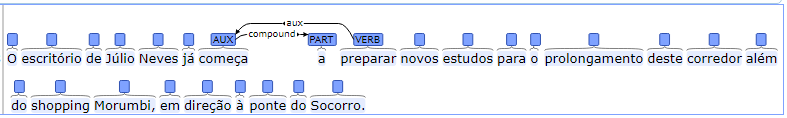
\includegraphics[width=\textwidth,height=\textheight,keepaspectratio]{imagesDrive/image26.png}
	    	\caption{Certo é que Pinochet fez do país uma casa portuguesa, com certeza}
	    	\label{fig:equesemMWE4}
	    	\end{figure}{}

\section{Predicativos e predicados verbo-nominais}\label{sec:predicativos}

	Os predicativos do sujeito em orações com verbo ser ou estar (funcionando como verbo de ligação, ver \fullref{sec:verbosauxiliares}), serão o núcleo da oração. Ou seja, em \say{O sorvete está gelado}, o núcleo (deprel \emph{root}) será \say{gelado}.

	 \fullref{dep:predicativodosujeito1}

	Em predicados verbo-nominais, os predicativos do objeto recebem classes diferentes caso sejam subordinados ao objeto ou ao verbo, conforme \fullref{sec:pintouamodelonua} e \fullref{sec:declarouoreuculpado}.
	
	\begin{figure}[H]
		\centering
		\vspace{.8cm}
		\begin{dependency}
			\begin{deptext}
				DET \& NOUN \& AUX \& VERB \& ADP \& NOUN \\
				Os \& arquivos \& são \& protegidos \& por \& senha \\
				o \& arquivo \& ser \& proteger \& por \& senha \\
			\end{deptext}
			\deproot{4}{root}
			\depedge{4}{3}{aux:pass}
			\depedge{4}{2}{nsubj}
			\depedge{2}{1}{det}
			\depedge{6}{5}{case}
			\depedge{4}{6}{obl:agent}
		\end{dependency}
		\caption{Os arquivos são \emph{protegidos} por senhas}\label{dep:predicativodosujeito1}
	\end{figure}

	\subsection{Ele pintou a modelo \emph{nua} e Ele entrou na sala \emph{cabisbaixo}: predicativo do sujeito e do objeto em predicados verbo-nominais}\label{sec:pintouamodelonua}

		Assim como o predicativo do sujeito, o predicativo do objeto em predicados verbo-nominais deve ter deprel \emph{acl}, como na \fullref{dep:pintouamodelonua}, em que nua é \emph{acl} e depende da palavra  modelo, uma vez que a frase é equivalente a pintou a modelo, e ela estava nua.

		Outro exemplo é \say{Ele entrou na sala cabisbaixo}, em que cabisbaixo é \emph{acl}, e depende de/modifica o sujeito ele.

		Por outro lado, em casos de verbos transitivos-predicativos (xingar, nomear, declarar etc), o predicativo é dependente do verbo, e será anotado como \emph{xcomp}, conforme \fullref{sec:declarouoreuculpado}.

		\begin{figure}[H]
			\centering
			\vspace{.8cm}
			\begin{dependency}
				\begin{deptext}
					VERB \& DET \& NOUN \& ADJ \\
					Pintou \& a \& modelo \& nua \\
					pintar \& o \& modelo \& nu \\
				\end{deptext}
				\deproot{1}{root}
				\depedge{1}{3}{obj}
				\depedge{3}{2}{det}
				\depedge{3}{4}{acl}
			\end{dependency}
			\caption{Pintou a modelo \emph{nua}}\label{dep:pintouamodelonua}
		\end{figure}

	\subsection{Declarou o réu \emph{culpado}: predicativos em verbos transitivos-predicativos}\label{sec:declarouoreuculpado}

		Quando o predicativo do objeto é dependentede verbos chamados transitivos-predicativos (achar, acusar; chamar; declarar; eleger (o povo o elegeu senador); supor; tachar; ter (todos o tinham como doido), estamos diante de um caso de \fullref{sec:argumentosdoverbo}, que deve ter deprel \emph{xcomp}, como na \fullref{dep:declarouoreuculpado} e na \fullref{dep:euoconsideroidiota}.
	
		Na frase \fullref{dep:xcomp4}, além do \say{deixando} que é \emph{xcomp} (objeto oracional), há também o \say{extenso} que tem deprel \emph{xcomp} por ser predicativo do objeto \say{currículo} ao mesmo tempo que argumento do verbo \emph{deixando}.
	
		\begin{figure}[H]
			\centering
			\vspace{.8cm}
			\begin{dependency}
				\begin{deptext}
					VERB \& DET \& NOUN \& ADJ \\
					Declarou \& o \& réu \& culpado \\
					declarar \& o \& réu \& culpado \\
				\end{deptext}
				\deproot{1}{root}
				\depedge{1}{3}{obj}
				\depedge{1}{4}{xcomp}
				\depedge{3}{2}{det}
			\end{dependency}
			\caption{Declarou o réu \emph{culpado}}\label{dep:declarouoreuculpado}
		\end{figure}
	
		\begin{figure}[H]
			\centering
			\vspace{.8cm}
			\begin{dependency}
				\begin{deptext}
					PRON \& PRON \& VERB \& ADJ \\
					Eu \& o \& considero \& idiota \\
					eu \& ele \& considero \& idiota \\
				\end{deptext}
				\deproot{3}{root}
				\depedge{3}{2}{obj}
				\depedge{3}{1}{nsubj}
				\depedge{3}{4}{xcomp}
			\end{dependency}
			\caption{Eu o considero \emph{idiota}}\label{dep:euoconsideroidiota}
		\end{figure}

\section{Argumentos do verbo}\label{sec:argumentosdoverbo}

	\subsection{Objeto direto e indireto}\label{sec:objetonominal}

		Em UD, caso o verbo possua apenas um objeto, esse objeto deve obrigatoriamente ser direto (deprel \emph{obj}), independentemente da presença ou não de preposição, como na \fullref{dep:objapenas}, que tem anotação igual à \fullref{dep:objapenas2}.

		Caso haja mais de um objeto, o primeiro será direto (seja ele nominal ou oracional), e o segundo, indireto (deprel \emph{iobj}), assim como na \fullref{dep:objeiobj}.

		O objeto indireto prototípico é aquele que é beneficiário/destinatário da ação do verbo, independente da posição que ocupe, como na \fullref{dep:iobjprototipico}. Assim, ainda que \say{aos réus} seja, linearmente, o 1º objeto, ele será \emph{iobj}.

		\begin{figure}[H]
			\centering
			\vspace{.8cm}
			\begin{dependency}
				\begin{deptext}
					PRON \& VERB \& PRON \\
					Eu \& adoro \& você \\
					eu \& adorar \& você \\
				\end{deptext}
				\deproot{2}{root}
				\depedge{2}{3}{obj}
				\depedge{2}{1}{nsubj}
			\end{dependency}
			\caption{Eu adoro \emph{você}}\label{dep:objapenas}
		\end{figure}

		\begin{figure}[H]
			\centering
			\vspace{.8cm}
			\begin{dependency}
				\begin{deptext}
					PRON \& VERB \& ADP \& PRON \\
					Eu \& gosto \& de \& você \\
					eu \& gostar \& de \& você \\
				\end{deptext}
				\deproot{2}{root}
				\depedge{2}{1}{nsubj}
				\depedge{2}{4}{obj}
				\depedge{4}{3}{case}
			\end{dependency}
			\caption{Eu gosto de \emph{você}}\label{dep:objapenas2}
		\end{figure}

		\begin{figure}[H]
			\centering
			\vspace{.8cm}
			\begin{dependency}
				\begin{deptext}
					DET \& NOUN \& VERB \& PRON \& DET \& NOUN \& ADP \& NOUN \& ADP \& DET \& NOUN \\
					O \& atacante \& pediu \& mais \& um \& dia \& de \& folga \& a \& o \& treinador \\
					o \& atacante \& pedir \& mais \& um \& dia \& de \& folga \& a \& o \& treinador \\
					\& \& \& PronType=Ind \\
				\end{deptext}
				\deproot{3}{root}
				\depedge{2}{1}{det}
				\depedge{3}{2}{nsubj}
				\depedge{6}{5}{det}
				\depedge{5}{4}{det}
				\depedge{3}{6}{obj}
				\depedge{8}{7}{case}
				\depedge{6}{8}{nmod}
				\depedge{3}{11}{iobj}
				\depedge{11}{10}{det}
				\depedge{11}{9}{case}
			\end{dependency}
			\caption{O atacante pediu mais um \emph{dia} de folga ao \emph{treinador}}\label{dep:objeiobj}
		\end{figure}

		\begin{figure}[H]
			\centering
			\vspace{.8cm}
			\begin{dependency}
				\begin{deptext}
					PROPN \& VERB \& ADP \& DET \& NOUN \& DET \& NOUN \& SCONJ \& VERB \\
					Souza \& negou \& a \& os \& réus \& o \& direito \& de \& apelarem \\
					Souza \& negar \& a \& o \& réu \& o \& direito \& de \& apelar \\
				\end{deptext}
				\deproot{2}{root}
				\depedge{2}{1}{nsubj}
				\depedge{2}{5}{iobj}
				\depedge{5}{4}{det}
				\depedge{5}{3}{case}
				\depedge{2}{7}{obj}
				\depedge{7}{6}{det}
				\depedge{7}{9}{acl}
				\depedge{9}{8}{mark}
			\end{dependency}
			\caption{Souza negou aos \emph{réus} o \emph{direito} de apelarem}\label{dep:iobjprototipico}
		\end{figure}


	\subsection{Caso o argumento do verbo seja uma oração (oração subordinada substantiva objetiva)}\label{sec:objetooracional}
	
		O objeto oracional é uma oração subordinada substantiva objetiva (direta ou indireta). Em UD, não há nenhuma diferenciação entre a anotação da oração objetiva direta e a indireta, mas deve-se notar outras diferenças em relação à análise das gramáticas do português.

		Orações subordinadas substantivas objetivas devem receber a deprel \emph{ccomp}, como na \fullref{dep:ccomp} e na \fullref{dep:ccomp2}.

		Em UD, quando o sujeito da oração subordinada é, obrigatoriamente, o mesmo sujeito da oração principal, usamos \emph{xcomp}. 
		
		São casos em que se poderia defender a presença de uma locução verbal, como em\say{decidiu adquirir}; \say{precisar fazer}, \say{querer comprar} (cf. locução verbal), ou de orações subordinadas reduzidas (disse saber; afirmou lamentar) mas que são anotados como \emph{xcomp}.
		
		 \fullref{dep:xcomp1}

		\fullref{dep:xcomp2}

		\fullref{dep:xcomp3}

		\fullref{dep:xcomp4}

		Esses casos, porém, não devem ser confundidos com os de sujeito oculto quando a oração é desenvolvida (ou seja, há a conjunção subordinativa), como na \fullref{dep:xcompsujeitooculto}.

		Outro caso de argumento do verbo que deve receber deprel \emph{xcomp}, embora seja nominal, é o dos predicativos do objeto quando são subordinados ao verbo, e não ao objeto, conforme \fullref{sec:declarouoreuculpado}.

		\begin{figure}[H]
			\centering
			\vspace{.8cm}
			\begin{dependency}
				\begin{deptext}
					VERB \& ADP \& DET \& NOUN \& SCONJ \& PRON \& VERB \\
					Pediu \& a \& os \& presentes \& que \& se \& empenhem \\
					pedir \& a \& o \& presente \& que \& se \& empenhar \\
				\end{deptext}
				\deproot{1}{root}
				\depedge{1}{4}{iobj}
				\depedge{4}{3}{det}
				\depedge{4}{2}{case}
				\depedge{1}{7}{ccomp}
				\depedge{7}{6}{expl}
				\depedge{7}{5}{mark}
			\end{dependency}
			\caption{Pediu aos presentes que se \emph{empenhem}}\label{dep:ccomp}
		\end{figure}

		\begin{figure}[H]
			\centering
			\vspace{.8cm}
			\begin{dependency}
				\begin{deptext}
					DET \& NOUN \& VERB \& DET \& PROPN \& VERB \& ADP \& DET \& NOUN \\
					Os \& eleitores \& querem \& o \& PT \& participando \& de \& o \& governo \\
					o \& eleitor \& quer \& o \& PT \& participar \& de \& o \& governo \\
				\end{deptext}
				\deproot{3}{root}
				\depedge{3}{2}{nsubj}
				\depedge{3}{5}{obj}
				\depedge{3}{6}{ccomp}
				\depedge{6}{9}{obl}
				\depedge{2}{1}{det}
				\depedge{5}{4}{det}
				\depedge{9}{8}{det}
				\depedge{9}{7}{case}
			\end{dependency}
			\caption{Os eleitores querem o PT \emph{participando} do governo}\label{dep:ccomp2}
		\end{figure}

		\begin{figure}[H]
			\centering
			\vspace{.8cm}
			\begin{dependency}
				\begin{deptext}
					DET \& NOUN \& VERB \& PRON \& SCONJ \& VERB \& DET \& NOUN \& ADP \& PROPN \\
					Os \& temas \& destinam \& se \& a \& mostrar \& o \& papel \& de \& Portugal \\
					o \& tema \& destinar \& se \& a \& mostrar \& o \& papel \& de \& Portugal \\
				\end{deptext}
				\deproot{3}{root}
				\depedge{3}{2}{nsubj}
				\depedge{3}{6}{xcomp}
				\depedge{6}{8}{obj}
				\depedge{8}{10}{nmod}
				\depedge{2}{1}{det}
				\depedge{3}{4}{expl}
				\depedge{6}{5}{mark}
				\depedge{8}{7}{det}
				\depedge{10}{9}{case}
			\end{dependency}
			\caption{Os temas destinam-se a \emph{mostrar} o papel de Portugal}\label{dep:xcomp1}
		\end{figure}

		\begin{figure}[H]
			\centering
			\vspace{.8cm}
			\begin{dependency}
				\begin{deptext}
					DET \& NOUN \& VERB \& SCONJ \& VERB \& NOUN \\
					O \& rendimento \& destinado \& a \& garantir \& condições \\
					o \& rendimento \& destinar \& a \& garantir \& condição \\
				\end{deptext}
				\deproot{3}{root}
				\depedge{3}{2}{nsubj}
				\depedge{3}{5}{xcomp}
				\depedge{5}{6}{obj}
				\depedge{2}{1}{det}
				\depedge{5}{4}{mark}
			\end{dependency}
			\caption{O rendimento destinado a \emph{garantir} condições}\label{dep:xcomp2}
		\end{figure}

		\begin{figure}[H]
			\centering
			\vspace{.8cm}
			\begin{dependency}
				\begin{deptext}
					PROPN \& PROPN \& VERB \& VERB \& ADP \& PROPN \\
					Netscape \& Communications \& decidiu \& adquirir \& a \& Collabra \\
					Netscape \& Communications \& decidir \& adquirir \& a \& Collabra \\
				\end{deptext}
				\deproot{3}{root}
				\depedge{3}{1}{nsubj}
				\depedge{3}{4}{xcomp}
				\depedge{4}{6}{obj}
				\depedge{1}{2}{flat:name}
				\depedge{6}{5}{det}
			\end{dependency}
			\caption{Netscape Communications decidiu \emph{adquirir} a Collabra}\label{dep:xcomp3}
		\end{figure}

		\begin{figure}[H]
			\centering
			\vspace{.8cm}
			\begin{dependency}
				\begin{deptext}
					PRON \& PRON \& VERB \& VERB \& DET \& NOUN \& ADJ \\
					O \& que \& acaba \& deixando \& o \& currículo \& extenso \\
					o \& que \& acabar \& deixar \& o \& currículo \& extenso \\
					PronType=Dem \& PronType=Rel \\
				\end{deptext}
				\deproot{1}{root}
				\depedge{1}{3}{acl:relcl}
				\depedge{3}{2}{nsubj}
				\depedge{3}{4}{xcomp}
				\depedge{4}{6}{obj}
				\depedge{6}{5}{det}
				\depedge{4}{7}{xcomp}
			\end{dependency}
			\caption{o que acaba \emph{deixando} o currículo extenso}\label{dep:xcomp4}
		\end{figure}

		\begin{figure}[H]
			\centering
			\vspace{.8cm}
			\begin{dependency}
				\begin{deptext}
					PRON \& VERB \& SCONJ \& VERB \\
					Ele \& disse \& que \& viria \\
					ele \& dizer \& que \& vir \\
				\end{deptext}
				\deproot{2}{root}
				\depedge{2}{1}{nsubj}
				\depedge{4}{3}{mark}
				\depedge{2}{4}{ccomp}
			\end{dependency}
			\caption{Ele disse que \emph{viria}}\label{dep:xcompsujeitooculto}
		\end{figure}
		
\section{Adjunto adverbiais}\label{sec:adjadv}

	UD oferece tratamentos diferentes para adjuntos adverbiais que são advérbios e adjuntos adverbiais formados por sintagmas nominais.
	
	\fullref{sec:adjadvadv}
	
	\fullref{sec:adjadvnome}
	
	\fullref{sec:adjadvverb}

		\subsection{Caso o adjunto adverbial seja advérbio}\label{sec:adjadvadv}
		
			O advérbio, que recebe upos \emph{ADV}, será anotado com a deprel \emph{advmod}.

			Como exemplo de modificador de \emph{VERB}, observa-se a \fullref{fig:advmod1}.

			Como exemplo de modificador de \emph{ADJ}, observa-se a \fullref{fig:advmod2}.

			Como exemplo de modificador de \emph{ADV}, observa-se a \fullref{fig:advmod3}.
	
			\begin{figure}[H]
				\centering
				\vspace{.8cm}
				\begin{dependency}
					\begin{deptext}
						DET\& NOUN\& AUX\& VERB\& ADV\\
						A\& limpeza\& é\& feita\& diariamente\\
						o\& limpeza\& ser\& fazer\& diariamente\\
					\end{deptext}
					
					\depedge{2}{1}{det}
					\depedge{4}{2}{nsubj:pass}
					\depedge{4}{3}{aux:pass}
					\deproot{4}{root}
					\depedge{4}{5}{advmod}
				\end{dependency}
				\caption{A limpeza é feita \emph{diariamente}}
				\label{fig:advmod1}
			\end{figure}
			
			\begin{figure}[H]
				\centering
				\vspace{.8cm}
				\begin{dependency}
					\begin{deptext}
						ADV\& VERB\& NOUN\& ADV\& ADJ\\
						Sempre\& tivemos\& canções\& mais\& lentas\\
						sempre\& ter\& canção\& mais\& lento\\
					\end{deptext}
					
					\depedge{2}{1}{advmod}
					\deproot{2}{root}
					\depedge{2}{3}{obj}
					\depedge{5}{4}{advmod}
					\depedge{3}{5}{nmod}
				\end{dependency}
				\caption{Sempre tivemos canções \emph{mais} lentas}
				\label{fig:advmod2}
			\end{figure}
		
			\begin{figure}[H]
				\centering
				\vspace{.8cm}
				\begin{dependency}
					\begin{deptext}
						ADV\& ADV\& VERB\& DET\& NOUN\& ADP\& DET\& NOUN\\
						Só\& assim\& evitarão\& a\& estratificação\& de\& a\& legislação\\
						só\& assim\& evitar\& o\& estratificação\& de\& a\& legislação\\
					\end{deptext}
					
					\depedge{2}{1}{advmod}
					\depedge{3}{2}{advmod}
					\deproot{3}{root}
					\depedge{5}{4}{det}
					\depedge{3}{5}{obj}
					\depedge{8}{6}{case}
					\depedge{8}{7}{det}
					\depedge{5}{8}{nmod}
					
				\end{dependency}
				\caption{\emph{Só} assim se evitará a estratificação da legislação}
				\label{fig:advmod3}
			\end{figure}
		
		\subsection{Caso o adjunto adverbial seja nome/sintagma nominal}\label{sec:adjadvnome}
			
			 O núcleo nominal de um adjunto adverbial (substantivo, pronome, sintagma nominal) será anotado como \emph{obl}. Ou seja, em \say{ele nadou ontem} temos advmod, mas em \say{ele nadou na piscina} temos obl.

			\fullref{fig:obl1}
	
			\fullref{fig:obl4}. 

			Como exemplo de modificador de \emph{ADJ}, observa-se a \fullref{fig:obl3}.

			Como exemplo de modificador de \emph{ADV}, observa-se a \fullref{fig:obl2}.

			\begin{figure}[H]
				\centering
				\vspace{.8cm}
				\begin{dependency}
					\begin{deptext}
						DET\& NOUN\& ADP\& DET\& NOUN\& VERB\& ADP\& DET\& NOUN\\
						A\& ideia\& para\& o\& livro\& surgiu\& após\& uma\& entrevista\\
						o\& ideia\& para\& o\& livro\& surgir\& após\& um\& entrevista\\
					\end{deptext}
					
					\depedge{2}{1}{det}
					\depedge{6}{2}{nsubj}
					\depedge{5}{3}{case}
					\depedge{5}{4}{det}
					\depedge{2}{5}{nmod}
					\deproot{6}{root}
					\depedge{9}{7}{case}
					\depedge{9}{8}{det}
					\depedge{6}{9}{obl}
				\end{dependency}
				\caption{A ideia para o livro surgiu após uma \emph{entrevista}}
				\label{fig:obl1}
			\end{figure}
			

			\begin{figure}[H]
				\centering
				\vspace{.8cm}
				\begin{dependency}
					\begin{deptext}
						ADV\& ADP\& DET\& NOUN\& ADJ\\
						Independentemente\& de\& o\& poder\& civil\\
						independentemente\& de\& o\& poder\& civil\\
					\end{deptext}					

					\deproot{1}{root}
					\depedge{4}{2}{case}
					\depedge{4}{3}{det}
					\depedge{1}{4}{obl}
					\depedge{4}{5}{amod}
				\end{dependency}
				\caption{Independentemente do \emph{poder} civil}
				\label{fig:obl2}
			\end{figure}

			\begin{figure}[H]
				\centering
				\vspace{.8cm}
				\begin{dependency}
					\begin{deptext}
						VERB\& SCONJ\& VERB\& NOUN\& ADV\& ADJ\& ADP\& DET\& NOUN\\
						Passaram\& a\& exigir\& funcionários\& mais\& abertos\& a\& o\& diálogo\\
						passar\& a\& exigir\& funcionário\& mais\& aberto\& a\& o\& diálogo\\
					\end{deptext}
					
					\deproot{1}{root}
					\depedge{3}{2}{mark}
					\depedge{1}{3}{xcomp}
					\depedge{3}{4}{obj}
					\depedge{6}{5}{advmod}
					\depedge{4}{6}{amod}
					\depedge{9}{7}{case}
					\depedge{9}{8}{det}
					\depedge{6}{9}{obl}
				\end{dependency}
				\caption{Passaram a exigir funcionários mais abertos ao \emph{diálogo}}
				\label{fig:obl3}
			\end{figure}

			\begin{figure}[H]
				\centering
				\vspace{.8cm}
				\begin{dependency}
					\begin{deptext}
						NOUN\& VERB\& ADP\& NOUN\& ADP\& DET\& NOUN\\
						Terrenos\& entregues\& como\& pagamento\& de\& uma\& dívida\\
						terrreno\& entregar\& como\& pagamento\& de\& um\& dívida\\
					\end{deptext}
					
					\deproot{1}{root}
					\depedge{1}{2}{acl}
					\depedge{4}{3}{case}
					\depedge{2}{4}{obl}
					\depedge{7}{5}{case}
					\depedge{7}{6}{det}
					\depedge{4}{7}{nmod}
		
				\end{dependency}
				\caption{Terrenos entregues como \emph{pagamento} de uma dívida}
				\label{fig:obl4}
			\end{figure}

			A relação de \emph{obl}, como é vista na \fullref{fig:obl3}, pode ser considerada um argumento de adjetivo (ver \fullref{sec:argumentosdoadjetivo}).
			
			A subrelação \emph{obl:agent} é utilizada para indicar o agente de um verbo na voz passiva. (ver \fullref{sec:vozpass}) 

		\subsection{Caso o adjunto adverbial seja uma oração}\label{sec:adjadvverb}
		
			A oração subordinada adverbial será anotada como \emph{advcl}, não havendo diferenciação semântica (temporal, causal, concessiva, final, etc). Poderá modificar \emph{VERB}.

			Nas estruturas comparativas, independente de o núcleo do fragmento ser um verbo ou um nome, ele será anotado com a deprel \emph{advcl} (ver \fullref{sec:estruturascomparativas}).

			\fullref{fig:advcl1}

			\fullref{fig:advcl2}

			\fullref{dep:quantomaiormenor}
			
			\begin{figure}[H]
				\centering
				\vspace{.8cm}
				\begin{dependency}
					\begin{deptext}
						SCONJ\& VERB\& DET\& NOUN\& PUNCT\& AUX\& DET\& ADJ\& NOUN\\
						Como\& notou\& o\& jornalista\& ,\& é\& uma\& boa\& grana\\
						como\& notar\& o\& jornalista\& ,\& ser\& um\& bom\& grana\\
					\end{deptext}
					
					\depedge{2}{1}{mark}
					\depedge{9}{2}{advcl}
					\depedge{4}{3}{det}
					\depedge{2}{4}{nsubj}
					\depedge{2}{5}{punct}
					\depedge{9}{6}{cop}
					\depedge{9}{7}{det}
					\depedge{9}{8}{amod}
					\deproot{9}{root}
				\end{dependency}
				\caption{Como \emph{notou} o jornalista, é uma boa grana}
				\label{fig:advcl1}
			\end{figure}

			\begin{figure}[H]
				\centering
				\vspace{.8cm}
				\begin{dependency}
					\begin{deptext}
						SCONJ\& PROPN\& VERB\& SCONJ\& VERB\& PUNCT\& VERB\& NOUN\\
						Quando\& Sarney\& começou\& a\& escrever\& ,\& chegaram\& protestos\\
						quando\& Sarney\& começar\& a\& escrever\& ,\& chegar\& protesto\\
					\end{deptext}
					
					\depedge{3}{1}{mark}
					\depedge{3}{2}{nsubj}
					\depedge{7}{3}{advcl}
					\depedge{5}{4}{mark}
					\depedge{3}{5}{xcomp}
					\depedge{3}{6}{punct}
					\deproot{7}{root}
					\depedge{7}{8}{nsubj}
				
				\end{dependency}
				\caption{Quando Sarney \emph{começou} a escrever, chegaram protestos}
				\label{fig:advcl2}
			\end{figure}

		\subsection{Teve uma relação extraconjugal com \emph{Monica} Lewinsky: quem é o pai?}\label{sec:terrelacaocom}
			Há casos em que é difícil saber se estamos diante de um argumento de verbo - ter [algo] [com alguém] - ou do nome ter [algo [com alguém]]. Na anotação, consideramos que \say{Monica} apontará para o verbo, e não para o nome. Sendo assim, o pai de \say{Monica} será \say{teve} e sua deprel será \emph{obl}.
			
			\fullref{dep:monica}
			
			\begin{figure}[H]
				\centering
				\vspace{.8cm}
				\begin{dependency}
					\begin{deptext}
						VERB\& DET\& NOUN\& ADJ\& ADP\& PROPN\& PROPN\\
						Teve\& uma\& relação\& extraconjugal\& com\& Monica\& Lewinsky\\
						ter\& um\& relação\& extraconjugal\& com\& Monica\& Lewinsky\\
					\end{deptext}
					
					\deproot{1}{root}
					\depedge{3}{2}{det}
					\depedge{1}{3}{obj}
					\depedge{3}{4}{amod}
					\depedge{6}{5}{case}
					\depedge{1}{6}{obl}
					\depedge{6}{7}{flat:name}
				
				\end{dependency}
				\caption{Teve uma relação extraconjugal com \emph{Monica} Lewinsky}
				\label{dep:monica}
			\end{figure}


\section{Adjuntos e argumentos do substantivo}\label{sec:adjuntoseargumentosdosubstantivo}

	Ver subseções:

	\fullref{sec:adjuntoadnominal}

	\fullref{sec:relativas}

	\fullref{sec:complementonominal}

	\fullref{sec:aposto}

	\subsection{Adjunto adnominal}\label{sec:adjuntoadnominal}

		Adjuntos adnominais são adjuntos (isto é, modificadores) de substantivos. Eles podem ser substantivos, adjetivos, numerais ou orações, e classificações sintáticas diferentes dependendo da sua classe gramatical.

		Caso sejam \emph{NOUN}, devem ter deprel \emph{nmod} (\fullref{dep:nmod}, e  \fullref{dep:nmod2}).

		Caso sejam \emph{ADJ}, devem ter deprel \emph{amod} (\fullref{dep:amod}).

		Caso sejam \emph{NUM}, devem ter deprel \emph{nummod} (\fullref{dep:nummod}). Ver também: \fullref{sec:numerais}.

		Sentenças como \fullref{dep:monica} são ambíguas, e privilegiamos leituras como \emph{obl} (\fullref{sec:terrelacaocom}).

		Sintagmas iniciados com preposição são sintagmas encaixados, como em \fullref{dep:epp}.

		\begin{figure}[H]
			\centering
			\vspace{.8cm}
			\begin{dependency}
				\begin{deptext}
					ADJ \& NUM \& NOUN \& ADP \& NOUN \& PUNCT \\
					Primeiros \& dois \& anos \& de \& mandato \& . \\
					primeiro \& dois \& ano \& de \& mandato \& . \\
					NumType=Ord \\
				\end{deptext}
				\deproot{3}{root}
				\depedge{3}{1}{amod}
				\depedge{3}{2}{nummod}
				\depedge{5}{4}{case}
				\depedge{3}{5}{nmod}
				\depedge{3}{6}{punct}
			\end{dependency}
			\caption{Primeiros dois anos de \emph{mandato}}\label{dep:nmod}
		\end{figure}

		\begin{figure}[H]
			\centering
			\vspace{.8cm}
			\begin{dependency}
				\begin{deptext}
					NOUN \& ADP \& NOUN \\
					Anel \& de \& ouro \\
					anel \& de \& ouro \\
				\end{deptext}
				\deproot{1}{root}
				\depedge{1}{3}{nmod}
				\depedge{3}{2}{case}
			\end{dependency}
			\caption{Anel de \emph{ouro}}\label{dep:nmod2}
		\end{figure}

		\begin{figure}[H]
			\centering
			\vspace{.8cm}
			\begin{dependency}
				\begin{deptext}
					NOUN \& ADJ \\
					Anel \& dourado \\
					anel \& dourado \\
				\end{deptext}
				\deproot{1}{root}
				\depedge{1}{2}{amod}
			\end{dependency}
			\caption{Anel \emph{dourado}}\label{dep:amod}
		\end{figure}

		\begin{figure}[H]
			\centering
			\vspace{.8cm}
			\begin{dependency}
				\begin{deptext}
					NUM \& NOUN \\
					3.600 \& concessionários \\
					3.600 \& concessionário \\
					NumType=Card \\
				\end{deptext}
				\deproot{2}{root}
				\depedge{2}{1}{nummod}
			\end{dependency}
			\caption{\emph{3.600} concessionários}\label{dep:nummod}
		\end{figure}

		\subsubsection{Orações relativas}\label{sec:relativas}

			Adjuntos adnominais na forma de orações (adjetivas/relativas) devem ter deprel \emph{acl:relcl} (que vem de \emph{adjective clause: relative clause}), caso sejam desenvolvidas (\fullref{dep:aclrelcl}), ou \emph{acl}, caso sejam reduzidas (\fullref{dep:acl}).

			\fullref{dep:aclrelclouacl1}

			\fullref{dep:aclrelclouacl2}

			\fullref{dep:aclrelclouacl3}

			\begin{figure}[H]
			        \centering
			        \vspace{.8cm}
			        \begin{dependency}
			                \begin{deptext}
			                        PRON \& AUX \& DET \& NOUN \& PRON \& VERB \& DET \& NOUN \& ADP \& DET \& NOUN  \\
			                        Esse \& é \& um \& fator \& que \& melhora \& o \& desempenho \& de \& o \& esportista \\
			                        esse \& ser \& um \& fator \& que \& melhorar \& o \& desempenho \& de \& o \& esportista \\
			                         \&  \&  \&  \&  \&  \&  \&  \&  \&  \&  \&  \\
			                         \&  \&  \&  \&  \&  \&  \&  \&  \&  \&  \&  \\
			                \end{deptext}
			                \depedge{4}{1}{nsubj}
			                \depedge{4}{2}{cop}
			                \depedge{4}{3}{det}
			                \deproot{4}{root}
			                \depedge{6}{5}{nsubj}
			                \depedge{4}{6}{acl:relcl}
			                \depedge{8}{7}{det}
			                \depedge{6}{8}{obj}
			                \depedge{11}{9}{case}
			                \depedge{11}{10}{det}
			                \depedge{8}{11}{nmod}
			        \end{dependency}
			        \caption{Esse é um fator que melhora o desempenho de o esportista}
			        \label{dep:aclrelcl}
			\end{figure}
	
			\begin{figure}[H]
			        \centering
			        \vspace{.8cm}
			        \begin{dependency}
			                \begin{deptext}
			                        DET \& NOUN \& VERB \& ADP \& DET \& NOUN \& AUX \& ADJ \& PUNCT \\
			                        O \& desempenho \& melhorado \& por \& a \& droga \& é \& ilegal \& . \\
			                        o \& desempenho \& melhorar \& por \& o \& droga \& ser \& ilegal \& . \\
			                         \&  \&  \&  \&  \&  \&  \&  \&  \\
			                         \&  \&  \&  \&  \&  \&  \&  \&  \\
			                \end{deptext}
			                \depedge{2}{1}{det}
			                \depedge{8}{2}{nsubj}
			                \depedge{2}{3}{acl}
			                \depedge{6}{4}{case}
			                \depedge{6}{5}{det}
			                \depedge{3}{6}{obl:agent}
			                \depedge{8}{7}{cop}
			                \deproot{8}{root}
			                \depedge{8}{9}{punct}
			        \end{dependency}
			        \caption{O desempenho melhorado por a droga é ilegal .}
			        \label{dep:acl}
			\end{figure}

			\begin{figure}[H]
			        \centering
			        \vspace{.8cm}
			        \begin{dependency}
			                \begin{deptext}
			                        DET \& NOUN \& PRON \& AUX \& DET \& NOUN \& PRON \& PROPN \& VERB \& PUNCT \\
			                        A \& casa \& amarela \& é \& a \& casa \& que \& Ana \& comprou \& . \\
			                        o \& casa \& amarelo \& ser \& o \& casa \& que \& Ana \& comprar \& . \\
			                         \&  \&  \&  \&  \&  \& PronType=Rel \&  \&  \&  \\
			                         \&  \&  \&  \&  \&  \&  \&  \&  \&  \\
			                \end{deptext}
			                \depedge{2}{1}{det}
			                \depedge{6}{2}{nsubj}
			                \depedge{6}{3}{nsubj}
			                \depedge{6}{4}{cop}
			                \depedge{6}{5}{det}
			                \deproot{6}{root}
			                \depedge{9}{7}{obj}
			                \depedge{9}{8}{nsubj}
			                \depedge{6}{9}{acl:relcl}
			                \depedge{6}{10}{punct}
			        \end{dependency}
			        \caption{A casa amarela é a casa que Ana comprou .}
			        \label{dep:aclrelclouacl1}
			\end{figure}

			\begin{figure}[H]
			        \centering
			        \vspace{.8cm}
			        \begin{dependency}
			                \begin{deptext}
			                        DET \& NOUN \& ADP \& PRON \& PRON \& VERB \& AUX \& PRON \& PUNCT \\
			                        A \& casa \& de \& que \& eu \& gosto \& é \& amarela \& . \\
			                        o \& casa \& de \& que \& eu \& gostar \& ser \& amarelo \& . \\
			                         \&  \&  \& PronType=Rel \&  \&  \&  \&  \&  \\
			                         \&  \&  \&  \&  \&  \&  \&  \&  \\
			                \end{deptext}
			                \depedge{2}{1}{det}
			                \depedge{8}{2}{nsubj}
			                \depedge{4}{3}{case}
			                \depedge{6}{4}{obj}
			                \depedge{6}{5}{nsubj}
			                \depedge{2}{6}{acl:relcl}
			                \depedge{8}{7}{cop}
			                \deproot{8}{root}
			                \depedge{2}{9}{punct}
			        \end{dependency}
			        \caption{A casa de que eu gosto é amarela .}
			        \label{dep:aclrelclouacl2}
			\end{figure}

			\begin{figure}[H]
			        \centering
			        \vspace{.8cm}
			        \begin{dependency}
			                \begin{deptext}
			                        DET \& NOUN \& VERB \& ADP \& DET \& PROPN \& AUX \& PRON \& PUNCT \\
			                        A \& casa \& comprada \& por \& a \& Ana \& é \& amarela \& . \\
			                        o \& casa \& comprar \& por \& o \& Ana \& ser \& amarelo \& . \\
			                         \&  \&  \&  \&  \&  \&  \&  \&  \\
			                         \&  \&  \&  \&  \&  \&  \&  \&  \\
			                \end{deptext}
			                \depedge{2}{1}{det}
			                \depedge{8}{2}{nsubj}
			                \depedge{2}{3}{acl}
			                \depedge{6}{4}{case}
			                \depedge{6}{5}{det}
			                \depedge{3}{6}{obl:agent}
			                \depedge{8}{7}{cop}
			                \deproot{8}{root}
			                \depedge{8}{9}{punct}
			        \end{dependency}
			        \caption{A casa comprada por a Ana é amarela .}
			        \label{dep:aclrelclouacl3}
			\end{figure}

	\subsection{Complemento nominal}\label{sec:complementonominal}

		Em UD, não há diferença entre complemento nominal ou adjunto adnominal, todos são nmod, de modo que \say{a compra da casa}, \say{a compra do mês} e \say{anel de ouro} são igualmente analisados como nmod. Outro exemplo é a \fullref{dep:complementonominal}.

		Ver \fullref{sec:adjuntoadnominal}.

		\begin{figure}[H]
			\centering
			\vspace{.8cm}
			\begin{dependency}
				\begin{deptext}
					NOUN \& ADP \& NOUN \\
					Medo \& de \& represálias \\
					medo \& de \& represália \\
				\end{deptext}
				\deproot{1}{root}
				\depedge{3}{2}{case}
				\depedge{1}{3}{nmod}
			\end{dependency}
			\caption{Medo de \emph{represálias}}\label{dep:complementonominal}
		\end{figure}

	\subsection{Aposto}\label{sec:aposto}

		Apostos, geralmente, apresentam uma relação de igualdade entre os nomes e verbos que relacionam.

		Tanto os apostos nominais (\fullref{dep:apostonominal1}, e \fullref{dep:apostonominal2}) como os oracionais (\fullref{dep:apostooracional}) recebem deprel \emph{appos}, sejam eles restritivos ou explicativos.

		Ainda que haja argumentos para uma anotação de adjunto adnominal, em casos como \say{o médico XXX}, \say{o grupo XXX} e \say{o parque XXX}, indicamos uma relação de aposto. Do mesmo modo, nomes científicos são tratados como \emph{appos} e \emph{compound}, como em \fullref{dep:nomecientif}.

		Ver também: \fullref{sec:mwe}

		Também estão em relação de aposto endereços de internet e e-mails, como em \fullref{dep:sitenet} e \fullref{dep:email}, respectivamente.

		\begin{figure}[H]
				\centering
				\vspace{.8cm}
				\begin{dependency}
					\begin{deptext}
						NOUN \& ADP \& DET \& NOUN \& ADP \& NOUN \& NOUN \& NOUN \\
						Microestruturas \& de \& os \& otólitos \& de \& arenques \& Clupea \& arengus \\
						microestrutura \& de \& o \& otólito \& de \& arenque \& Clupea \& arengus \\
					\end{deptext}
					\deproot{1}{root}
					\depedge{4}{2}{case}
					\depedge{4}{3}{det}
					\depedge{1}{4}{nmod}
					\depedge{6}{5}{case}
					\depedge{4}{6}{nmod}
					\depedge{6}{7}{appos}
					\depedge{7}{8}{compound}
				\end{dependency}
				\caption{Microestruturas dos otólitos de arenques \emph{Clupea arengus}}\label{dep:nomecientif}
			\end{figure}

			\begin{figure}[H]
				\centering
				\vspace{.8cm}
				\begin{dependency}
					\begin{deptext}
						DET \& NOUN \& VERB \& AUX \& VERB \& ADP \& DET \& NOUN \& NOUN\\
						O \& sistema \& pode \& ser \& acessado \& em \& o \& portal \& http://www.lei.furg.br/sidipla\\
						o \& sistema \& poder \& ser \& acessar \& em \& o \& portal \& http://www.lei.furg.br/sidipla\\
					\end{deptext}
					\depedge{2}{1}{det}
					\depedge{3}{2}{nsubj:pass}
					\deproot{3}{root}
					\depedge{5}{4}{aux:pass}
					\depedge{3}{5}{xcomp}
					\depedge{8}{6}{case}
					\depedge{8}{7}{det}
					\depedge{5}{8}{obl}
					\depedge{8}{9}{appos}
				\end{dependency}
				\caption{O sistema pode ser acessado no portal \emph{http://www.lei.furg.br/sidipla}}\label{dep:sitenet}
			\end{figure}

			\begin{figure}[H]
				\centering
				\vspace{.8cm}
				\begin{dependency}
					\begin{deptext}
						NOUN \& PUNCT \& NOUN \\
						Email \& : \& jones@abc.ed \\
						email \& : \& jones@abc.ed \\
					\end{deptext}
					\deproot{1}{root}
					\depedge{1}{2}{punct}
					\depedge{1}{3}{appos}
				\end{dependency}
				\caption{Email: \emph{jones@abc.ed}}\label{dep:email}
			\end{figure}

		Ver também: \fullref{sec:apostooque}, \fullref{sec:apostoenum} e \fullref{sec:apostotrad}

		\begin{figure}[H]
			\centering
			\vspace{.8cm}
			\begin{dependency}
				\begin{deptext}
					DET \& NOUN \& PUNCT \& PROPN \& PUNCT \& VERB \& DET \& NOUN \\
					O \& ministro \& , \& FHC \& , \& fez \& um \& pronunciamento \\
					o  \& ministro \& , \& FHC \& , \& fazer \& um \& pronunciamento \\
				\end{deptext}
				\deproot{6}{root}
				\depedge{6}{2}{nsubj}
				\depedge{6}{8}{obj}
				\depedge{2}{1}{det}
				\depedge{8}{7}{det}
				\depedge{4}{3}{punct}
				\depedge{4}{5}{punct}
				\depedge{2}{4}{appos}
			\end{dependency}
			\caption{O ministro, \emph{FHC}, fez um pronunciamento}\label{dep:apostonominal1}
		\end{figure}

		\begin{figure}[H]
			\centering
			\vspace{.8cm}
			\begin{dependency}
				\begin{deptext}
					VERB \& DET \& NOUN \& PROPN \\
					Afirmou \& o \& levantador \& Maurício \\
					afirmar \& o \& levantador \& Maurício \\
				\end{deptext}
				\deproot{1}{root}
				\depedge{1}{3}{nsubj}
				\depedge{3}{4}{appos}
				\depedge{3}{2}{det}
			\end{dependency}
			\caption{Afirmou o levantador \emph{Maurício}}\label{dep:apostonominal2}
		\end{figure}

		\begin{figure}[H]
			\centering
			\vspace{.8cm}
			\begin{dependency}
				\begin{deptext}
					DET \& NOUN \& PRON \& VERB \& PUNCT \& VERB \& NOUN \\
					A \& solução \& que \& deram \& , \& obter \& equilíbrio \\
					o \& solução \& que \& dar \& , \& obter \& equilíbrio \\ 
				\end{deptext}
				\deproot{2}{root}
				\depedge{2}{1}{det}
				\depedge{2}{4}{acl:relcl}
				\depedge{2}{6}{appos}
				\depedge{6}{7}{obj}
				\depedge{6}{5}{punct}
				\depedge{4}{3}{obj}
			\end{dependency}
			\caption{A solução que deram, \emph{obter} equilíbrio}\label{dep:apostooracional}
		\end{figure}

		\subsubsection{Aposto e dois pontos/enumeração}\label{sec:apostoenum}

			Em casos de aposto após dois pontos, como em uma enumeração, ele será anotado como \emph{appos}. Um exemplo encontra-se na \fullref{fig:apostoenum}.
			\begin{figure}[H]
			    	\centering
			    	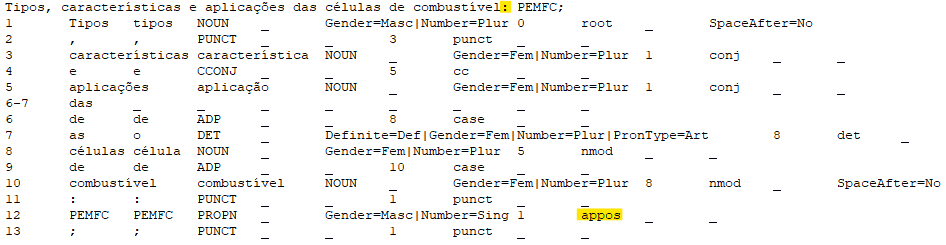
\includegraphics[width=\textwidth,height=\textheight,keepaspectratio]{imagesDrive/appos2.png}
			    	\caption{Tipos, características e aplicações das células de combustível: PEMFC;}
			    	\label{fig:apostoenum}
			\end{figure}{}

		\subsubsection{Aposto e traduções}\label{sec:apostotrad}

			As diretivas originais UD não especificam como anotar termos/expressões frases que são traduções. Em UD-PT, optamos por deixá-las como aposto: \fullref{fig:apostotrad}

			\begin{figure}[H]
			    	\centering
			    	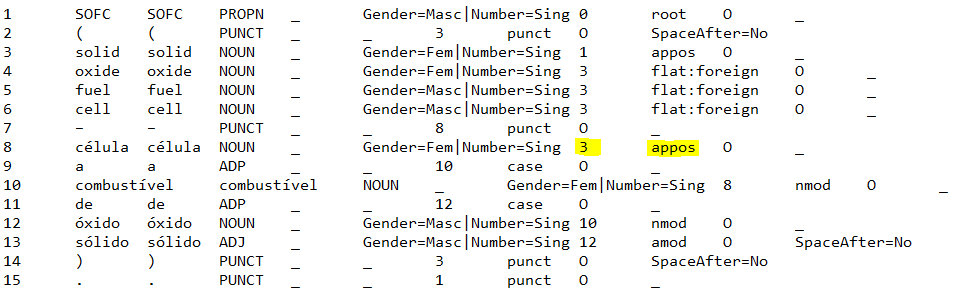
\includegraphics[width=\textwidth,height=\textheight,keepaspectratio]{imagesDrive/appos1.png}
			    	\caption{SOFC (solid oxide fuel cell – \emph{célula} a combustível de óxido sólido):}
			    	\label{fig:apostotrad}
			\end{figure}{}

		\subsubsection{Orações com '', o que''}\label{sec:apostooque}

			Em orações com a presença de \say{, o que}, analisamos o \say{o} como pronome demonstrativo, isto é, igual a \say{aquilo} (conforme \fullref{sec:amaisquerida}), funcionando como aposto da oração antecendente (\fullref{dep:apostooque}).

			\begin{figure}[H]
				\centering
				\vspace{.8cm}
				\begin{dependency}
					\begin{deptext}
						VERB \& DET \& NOUN \& ADP \& DET \& NOUN \& PUNCT \& PRON \& PRON \& PRON \& VERB \\
						Morreu \& o \& cachorro \& de \& a \& velha \& , \& o \& que \& a \& entristece \\
						morrer \& o \& cachorro \& de \& o \& velho \& , \& o \& que \& ela \& entristecer \\
					\end{deptext}
					\deproot{1}{root}
					\depedge{1}{3}{nsubj}
					\depedge{3}{2}{det}
					\depedge{6}{5}{det}
					\depedge{6}{4}{case}
					\depedge{3}{6}{nmod}
					\depedge{7}{8}{punct}
					\depedge{1}{8}{appos}
					\depedge{8}{11}{acl:relcl}
					\depedge{11}{9}{nsubj}
					\depedge{11}{10}{obj}
				\end{dependency}
				\caption{Morreu o cachorro da velha, \emph{o} que a entristece}\label{dep:apostooque}
			\end{figure}

		\subsubsection{Apostos coordenados}\label{sec:apostoscoordenados}

			Apostos coordenados são analisados como apostos dependentes da primeira palavra, e não como coordenações, como na \fullref{dep:apostoscoordenados}.

			\begin{figure}[H]
				\centering
				\vspace{.8cm}
				\begin{dependency}
					\begin{deptext}
						DET \& NOUN \& PUNCT \& PROPN \& PROPN \& PUNCT \& DET \& PUNCT \& PROPN \& PUNCT \\
						O \& réu \& , \& Alexandre \& Cardoso \& , \& o \& « \& Topeira \& » \\
						o \& réu \& , \& Alexandre \& Cardoso \& , \& o \& « \& Topeira \& » \\
						%Definite=Def \& NumType=Ord \\
						%PronType=Art \\
					\end{deptext}
					\deproot{2}{root}
					\depedge{2}{1}{det}
					\depedge{4}{3}{punct}
					\depedge{4}{5}{flat:name}
					\depedge{4}{6}{punct}
					\depedge{2}{4}{appos}
					\depedge{2}{9}{appos}
					\depedge{9}{8}{punct}
					\depedge{9}{7}{det}
					\depedge{9}{10}{punct}
				\end{dependency}
				\caption{O terceiro réu, \emph{Alexandre} Cardoso, o «\emph{Topeira}»}\label{dep:apostoscoordenados}
			\end{figure}

\section{Argumentos do adjetivo}\label{sec:argumentosdoadjetivo}
	
	Caso o complemento do adjetivo seja nominal, deve ter deprel \emph{obl}, conforme \fullref{dep:argumentoadjetivonominal}. Pode ser considerado um caso de adjunto adverbial (\fullref{sec:adjadv}).
	
	Caso o complemento do adjetivo seja oracional, deve ter deprel \emph{ccomp}, conforme \fullref{dep:argumentoadjetivooracional}.
	
	\begin{figure}[H]
	\centering
	\vspace{.8cm}
	\begin{dependency}
		\begin{deptext}
			DET \& NOUN \& VERB \& DET \& NOUN \& ADJ \& ADP \& DET \& NOUN \& PUNCT \\
			A \& reivindicação \& irritou \& os \& partidos \& favoráveis \& a \& a \& revisão \& . \\
			o \& reivindicação \& irritar \& o \& partido \& favorável \& a \& a \& revisão \& . \\
		\end{deptext}
		\deproot{3}{root}
		\depedge{3}{2}{nsubj}
		\depedge{2}{1}{det}
		\depedge{5}{4}{det}
		\depedge{3}{5}{obj}
		\depedge{5}{6}{amod}
		\depedge{9}{8}{case}
		\depedge{9}{7}{det}
		\depedge{3}{10}{punct}
		\depedge{6}{9}{obl}
	\end{dependency}
	\caption{Irritou os partidos favoráveis à \emph{revisão}}\label{dep:argumentoadjetivonominal}
\end{figure}

	\begin{figure}[H]
		\centering
		\vspace{.8cm}
		\begin{dependency}
			\begin{deptext}
				VERB \& DET \& NOUN \& ADJ \& SCONJ \& VERB \& NOUN \& PUNCT \\
				Irritou \& os \& partidos \& favoráveis \& a \& rever \& candidaturas \& . \\
				irritar \& o \& partido \& favorável \& a \& rever \& candidatura \& . \\
			\end{deptext}
			\deproot{1}{root}
			\depedge{3}{2}{det}
			\depedge{1}{3}{obj}
			\depedge{3}{4}{amod}
			\depedge{6}{5}{mark}
			\depedge{1}{8}{punct}
			\depedge{4}{6}{ccomp}
			\depedge{6}{7}{obj}
		\end{dependency}
		\caption{Irritou os partidos favoráveis a \emph{rever} candidaturas}\label{dep:argumentoadjetivooracional}
	\end{figure}
	
	

\section{Locuções verbais}\label{sec:deplocverbal}

	Locuções verbais são os casos de dois verbos em que o primeiro tem upos \emph{AUX}, e o segundo, \emph{VERB}, sendo o primeiro um verbo auxiliar e o segundo, verbo pleno. O verbo auxiliar irá apontar para o verbo principal, ou seja, o núcleo da oração é o VERB. Exemplo. O que conta como uma locução verbal é alvo de muita discussão linguística, sobretudo no que se refere às locuções modais (\say{eu quis fazer a prova}). Para identificar os casos de locução verbal, consultar \fullref{sec:verbosauxiliares}. Em UD, construções que poderiam também ser consideradas locução verbal são anotadas como xcomp (que é o caso de \say{eu quis fazer a prova}, por exemplo). Ver mais sobre xcomp na \fullref{sec:predicativos}.

\section{Voz passiva}\label{sec:vozpass}

	Na voz passiva, anota-se o sujeito com a deprel \emph{nsubj:pass}, e o agente da passiva, com a deprel \emph{obl:agent}. O verbo \say{ser}, como explicitado na \fullref{sec:servozpassiva}, recebe upos \emph{AUX} e deprel \emph{aux:pass}. 
	
	\fullref{fig:vozpass1}
	
	\fullref{fig:vozpass2}	

	\begin{figure}[H]
		\centering
		\vspace{.8cm}
		\begin{dependency}
			\begin{deptext}
				DET\& PROPN\& AUX\& VERB\& ADP\& NUM\& NOUN\\
				A\& URV\& é\& produzida\& por\& três\& índices\\
				o\& URV\& ser\& produzir\& por\& três\& índice\\
			\end{deptext}
			
			\depedge{2}{1}{det}
			\depedge{4}{2}{nsubj:pass}
			\depedge{4}{3}{aux:pass}
			\deproot{4}{root}
			\depedge{7}{5}{case}
			\depedge{7}{6}{nummod}
			\depedge{4}{7}{obl:agent}

		\end{dependency}
		\caption{A URV é produzida por três índices}
		\label{fig:vozpass1}
	\end{figure}

	\begin{figure}[H]
		\centering
		\vspace{.8cm}
		\begin{dependency}
			\begin{deptext}
				DET\& NOUN\& VERB\& AUX\& VERB\& ADP\& DET\& NOUN\\
				O\& trabalho\& pode\& ser\& feito\& por\& qualquer\& pessoa\\
				o\& trabalho\& poder\& ser\& fazer\& por\& qualquer\& pessoa\\
			\end{deptext}
			
			\depedge{2}{1}{det}
			\depedge{3}{2}{nsubj:pass}
			\deproot{3}{root}
			\depedge{5}{4}{aux:pass}
			\depedge{3}{5}{xcomp}
			\depedge{8}{6}{case}
			\depedge{8}{7}{det}
			\depedge{3}{8}{obl:agent}
		\end{dependency}
		\caption{O trabalho pode ser feito por qualquer pessoa}
		\label{fig:vozpass2}
	\end{figure}


\section{Discurso direto}\label{sec:discursodireto}

	Discurso direto é anotado como de deprel \emph{parataxis}, pois não há uma conexão formal, explícita, entre as duas orações.

	Assim, se \say{«É uma \emph{coisa} do Primeiro Mundo», afirmou} é \emph{parataxis}, \say{Afirmou que é uma \emph{coisa} de outro mundo} é \emph{ccomp}.

	\fullref{dep:discursodireto}

	Ver também \fullref{sec:parataxis}.


	\begin{figure}[H]
		\centering
		\vspace{.8cm}
		\begin{dependency}
			\begin{deptext}
				PUNCT \& AUX \& DET \& NOUN \& ADP \& DET \& ADJ \& NOUN \& PUNCT \& PUNCT \& VERB \\
				« \& É \& uma \& coisa \& de \& o \& Primeiro \& Mundo \& » \& , \& afirmou \\
				« \& ser \& uma \& coisa \& de \& o \& primeiro \& mundo \& » \& , \& afirmar \\
			\end{deptext}
			\deproot{11}{root}
			\depedge{11}{4}{parataxis}
			\depedge{4}{1}{punct}
			\depedge{4}{9}{punct}
			\depedge{4}{10}{punct}
			\depedge{4}{2}{aux}
			\depedge{4}{3}{det}
			\depedge{8}{7}{amod}
			\depedge{8}{6}{det}
			\depedge{8}{5}{case}
			\depedge{4}{8}{nmod}
		\end{dependency}
		\caption{«É uma \emph{coisa} do Primeiro Mundo», afirmou}\label{dep:discursodireto}
	\end{figure}

	\section{Estruturas comparativas}\label{sec:estruturascomparativas}

	Estruturas comparativas são de anotação complexa, o que se verifica pela existência de um \href{https://universaldependencies.org/workgroups/comparatives.html}{working group (WG) em UD} dedicado especialmente a elas. A seguir, listamos as frases utilizadas no WG, traduzidas em português, e com a anotação adequada, além de algumas frases de anotação complexa no Bosque-UD.

	\subsection{Frases do Working Group}

	\fullref{fig:comparative1}

	\fullref{fig:comparative2}

	\fullref{fig:comparative3}

	\fullref{fig:comparative4}
	
	\begin{figure}[H]
	    \centering
	    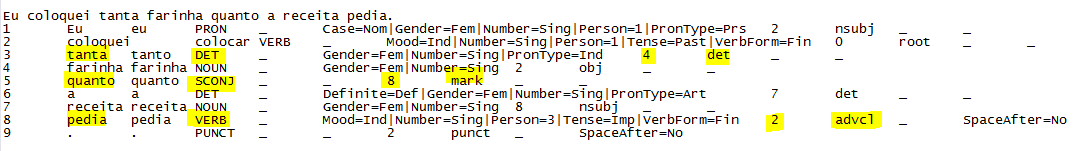
\includegraphics[width=\textwidth,height=\textheight,keepaspectratio]{imagesDrive/image23.png}
	    \caption{Eu coloquei \emph{tanta farinha quanto} a receita pedia}
	    \label{fig:comparative1}
	    \end{figure}{}
	
	\begin{figure}[H]
	    \centering
	    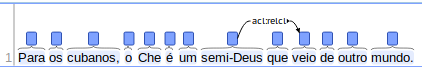
\includegraphics[width=\textwidth,height=\textheight,keepaspectratio]{imagesDrive/image32.png}
	    \caption{Martin é o cara \emph{mais inteligente de todos}}
	    \label{fig:comparative2}
	\end{figure}{}

	\begin{figure}[H]
	    \centering
	    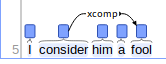
\includegraphics[width=\textwidth,height=\textheight,keepaspectratio]{imagesDrive/image44.png}
	    \caption{Ele toca \emph{melhor bêbado do que sóbrio}}
	    \label{fig:comparative3}
	\end{figure}{}

	\begin{figure}[H]
	    \centering
	    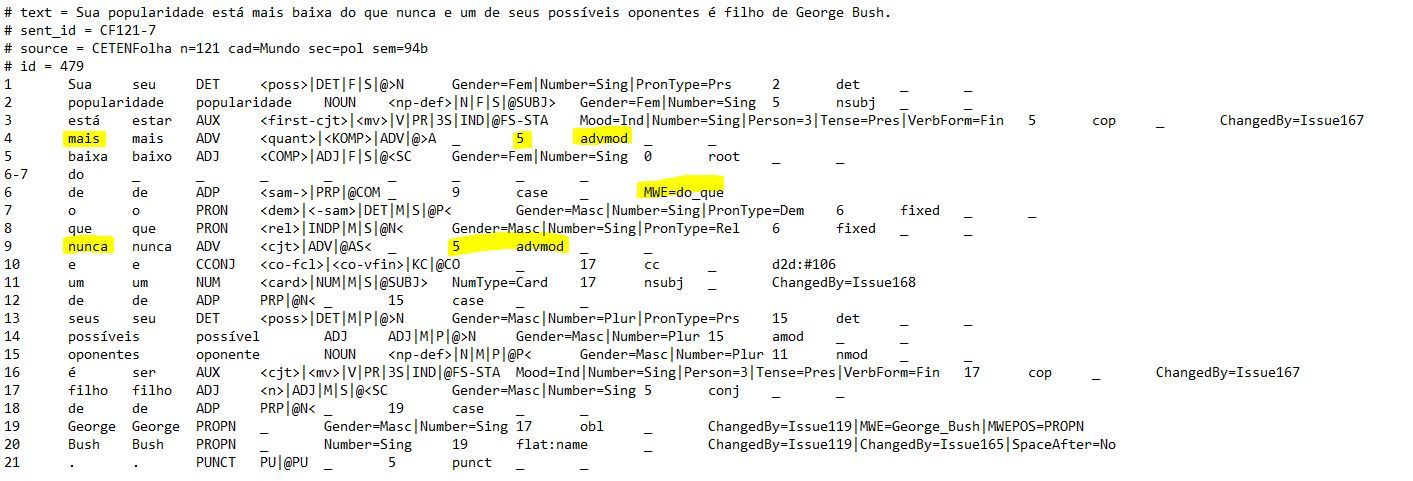
\includegraphics[width=\textwidth,height=\textheight,keepaspectratio]{imagesDrive/image35.png}
	    \caption{Matilda é \emph{mais gentil do que você pensa}}
	    \label{fig:comparative4}
	\end{figure}{}

\section{Relações que só existem em UD}

	\subsection{xcomp}

		\emph{xcomp} pode se referir a diferentes categorias da GT, como oração subordinada substantiva objetiva e predicativo do objeto. O que há em comum nas duas classificações é que, em ambos os casos, o \emph{xcomp} é dependente/subordinado a um verbo, invariavelmente.

		Ver também: \fullref{sec:objetooracional}

		Ver também: \fullref{sec:declarouoreuculpado}

	\subsection{cop}

		\emph{cop} é a deprel utilizada unicamente para verbos de ligação, mais especificamente, apenas \say{ser} e \say{estar}.

		Ver também: \fullref{sec:verbosdeligacao}

	\subsection{aux}

		\emph{aux} refere-se unicamente às locuções verbais de tempo composto.

		\emph{aux:pass}, por sua vez, ao verbo \say{ser} como voz passiva.

		Ver também: \fullref{sec:auxtempocomposto}

		Ver também: \fullref{sec:servozpassiva}

	\subsection{parataxis}

		\emph{parataxis} é a deprel utilizada quando a relação sintática entre duas orações não é explicitada na sentença.

		Ver também: \fullref{sec:parataxis}

	\subsection{fixed, compound, flat:name (MWE)}\label{sec:mwe}

		Há pelo menos três formas diferentes de indicar expressões multi-palavras (MWEs) em UD. Quando se trata de uma expressão estritamente gramatical, sem flexão, usamos a deprel \emph{fixed} (\fullref{dep:fixed}). Quando a expressão multi-palavra pode conter flexão, utilizamos a deprel \emph{compound} (\fullref{dep:compound}), e quando se trata de nome próprio de pessoa composto, utilizamos a deprel \emph{flat:name} (\fullref{dep:flatname}).

		Ver também: \fullref{sec:numeroscompostos}

		Ver também: \fullref{sec:nomeseguidodenome}

		\begin{figure}[H]
			\centering
			\vspace{.8cm}
			\begin{dependency}
				\begin{deptext}
					ADP \& DET \& NOUN \& VERB \& ADP \& NOUN \& ADP \& NOUN \\
					A \& as \& vezes \& peco \& por \& falta \& de \& experiência \\
					A \& o \& vez \& pecar \& por \& falta \& de \& experiência \\
				\end{deptext}
				\depedge{1}{2}{fixed}
				\depedge{1}{3}{fixed}
				\depedge{4}{1}{advmod}
				\depedge{4}{6}{obl}
				\depedge{6}{8}{nmod}
				\depedge{8}{7}{case}
				\depedge{6}{5}{case}
				\deproot{1}{root}
			\end{dependency}
			\caption{\emph{Às vezes} peco por falta de experiência}
			\label{dep:fixed}
		\end{figure}

		\begin{figure}[H]
			\centering
			\vspace{.8cm}
			\begin{dependency}
				\begin{deptext}
					PROPN \& ADP \& DET \& PROPN \& PROPN \\
					Secretaria \& de \& o \& Meio \& Ambiente \\
					Secretaria \& de \& o \& Meio \& Ambiente \\
				\end{deptext}
				\depedge{4}{3}{det}
				\depedge{4}{2}{case}
				\depedge{4}{5}{compound}
				\depedge{1}{4}{nmod}
				\deproot{1}{root}
			\end{dependency}
			\caption{Secretaria do Meio \emph{Ambiente}}
			\label{dep:compound}
		\end{figure}

		\begin{figure}[H]
			\centering
			\vspace{.8cm}
			\begin{dependency}
				\begin{deptext}
					DET \& NOUN \& VERB \& NOUN \& ADJ \& ADP \& PROPN \& PROPN \\
					o \& programa \& mostrará \& reportagens \& especiais \& de \& Sônia \& Pompeu \\
					o \& programa \& mostrar \& reportagem \& especial \& de \& Sônia \& Pompeu \\
				\end{deptext}
				\depedge{2}{1}{det}
				\depedge{3}{2}{nsubj}
				\depedge{3}{4}{obj}
				\depedge{4}{5}{amod}
				\depedge{7}{6}{case}
				\depedge{4}{7}{nmod}
				\depedge{7}{8}{flat:name}
				\deproot{3}{root}
			\end{dependency}
			\caption{o programa mostrará reportagens especiais de Sônia \emph{Pompeu}}
			\label{dep:flatname}
		\end{figure}

	\subsection{case}

		\emph{case} é a deprel utilizada pelas preposições. Elas, por sua vez, dependem/se subordinam sempre ao token à sua direita.

		Ver também: \fullref{sec:classesdinamicas}

		Ver também: \fullref{sec:preposicoes}
		
	\subsection{orphan}	
	
		\emph{orphan} é a deprel utilizada quando há elipse do núcleo (head) da oração, em situações cuja solução mais óbvia levaria a uma classificação inadequada. Esse caso poderia acontecer, por exemplo, na sentença da \fullref{fig:orphan-cigarros}, com \say{5} apontando para \say{mulher} como \emph{obj}; porém, \say{5} não é objeto de \say{mulher}. Em vez disso, usa-se a deprel \emph{orphan}. O pai do \emph{orphan} é promovido a núcleo e assume a relação \emph{conj} com o verbo da oração. Outro exemplo se encontra na \fullref{fig:orphan-graus}.
	
		\begin{figure}[H]
		    \centering
		    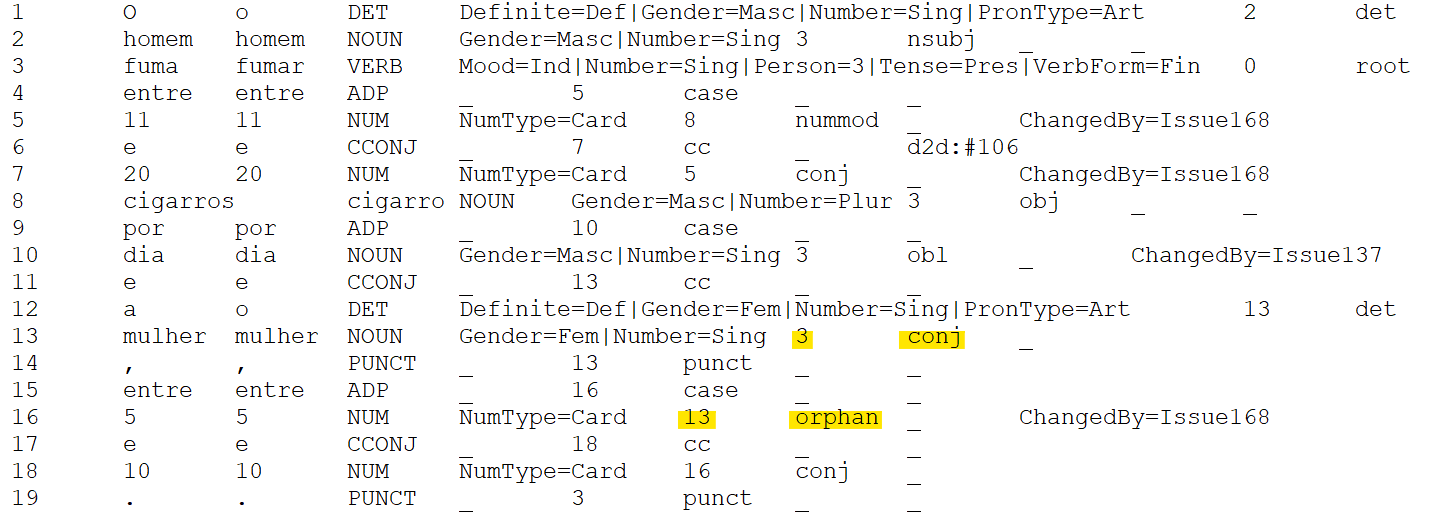
\includegraphics[width=\textwidth,height=\textheight,keepaspectratio]{imagesDrive/orphan-cigarros.png}
		    \caption{O homem fuma entre 11 e 20 cigarros por dia e a mulher, entre \emph{5} e 10.}
		    \label{fig:orphan-cigarros}
		\end{figure}{}	
	
		\begin{figure}[H]
		    \centering
		    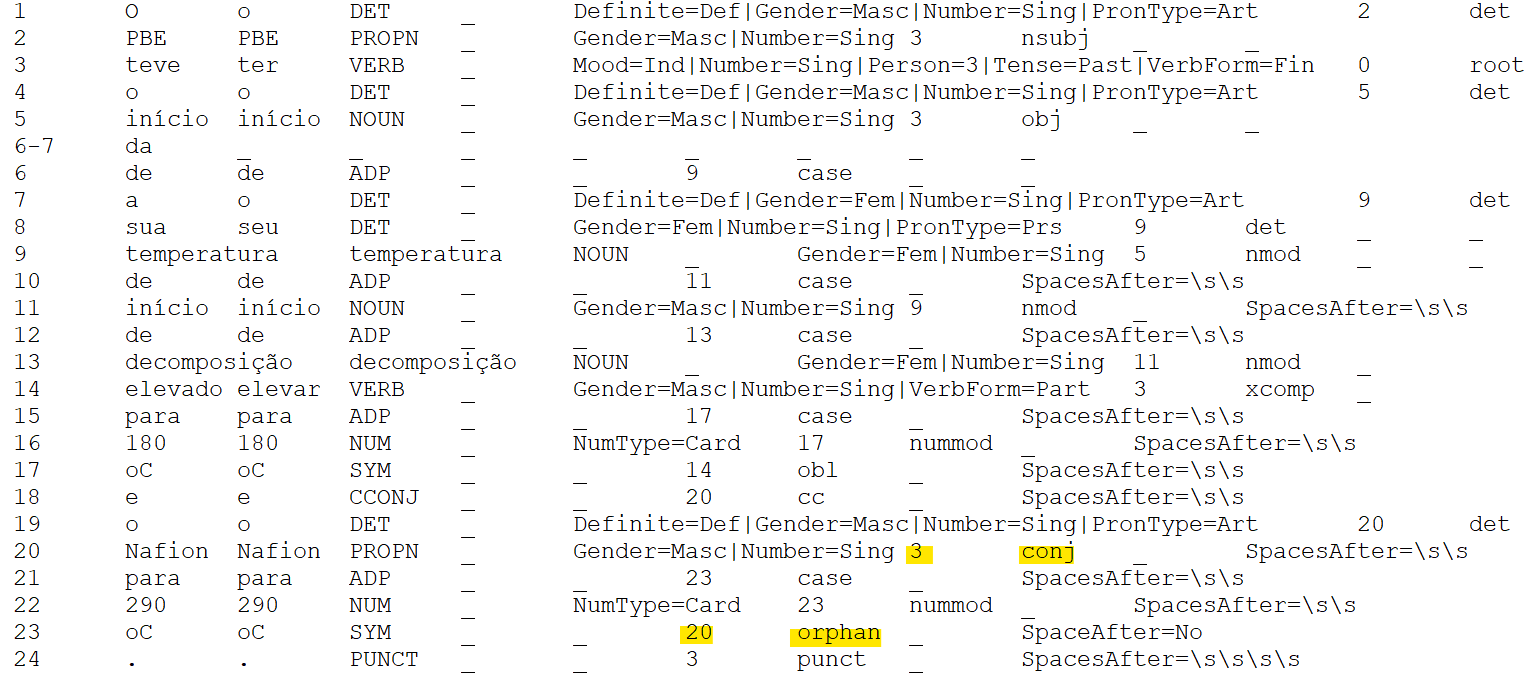
\includegraphics[width=\textwidth,height=\textheight,keepaspectratio]{imagesDrive/orphan-graus.png}
		    \caption{O PBE teve o início da sua temperatura de início de decomposição elevado para 180 oC e o Nafion para 290 \emph{oC}.}
		    \label{fig:orphan-graus}
		\end{figure}{}	

\chapter{Frases difíceis}
\hyperlink{toc}{Ir para tabela de conteúdos\\}

	\section{Adverbial proporcional}

		\fullref{dep:quantomaiormenor}

		\begin{figure}[H]
		        \centering
		        \vspace{.8cm}
		        \begin{dependency}
		                \begin{deptext}
		                        ADV \& ADJ \& DET \& NOUN \& PUNCT \& ADJ \& DET \& NOUN \& ADP \& NOUN \\
		                        Quanto \& maior \& a \& concentração \& , \& menor \& a \& invasão \& de \& filtrado \\
		                        quanto \& maior \& o \& concentração \& , \& pequeno \& o \& invasão \& de \& filtrado \\
		                         \&  \&  \&  \&  \&  \&  \&  \&  \&  \\
		                         \&  \&  \&  \&  \&  \&  \&  \&  \&  \\
		                \end{deptext}
		                \depedge{2}{1}{advmod}
		                \depedge{4}{2}{amod}
		                \depedge{4}{3}{det}
		                \depedge{8}{4}{advcl}
		                \depedge{6}{5}{punct}
		                \depedge{8}{6}{amod}
		                \depedge{8}{7}{det}
		                \deproot{8}{root}
		                \depedge{10}{9}{case}
		                \depedge{8}{10}{nmod}
		        \end{dependency}
		        \caption{Quanto maior a concentração , menor a invasão de filtrado}
		        \label{dep:quantomaiormenor}
		\end{figure}

	\section{Comparativas}

	\subsection{mais do que}

	\fullref{fig:comparative5}

	\fullref{fig:comparative6}

	\begin{figure}[H]
	    \centering
	    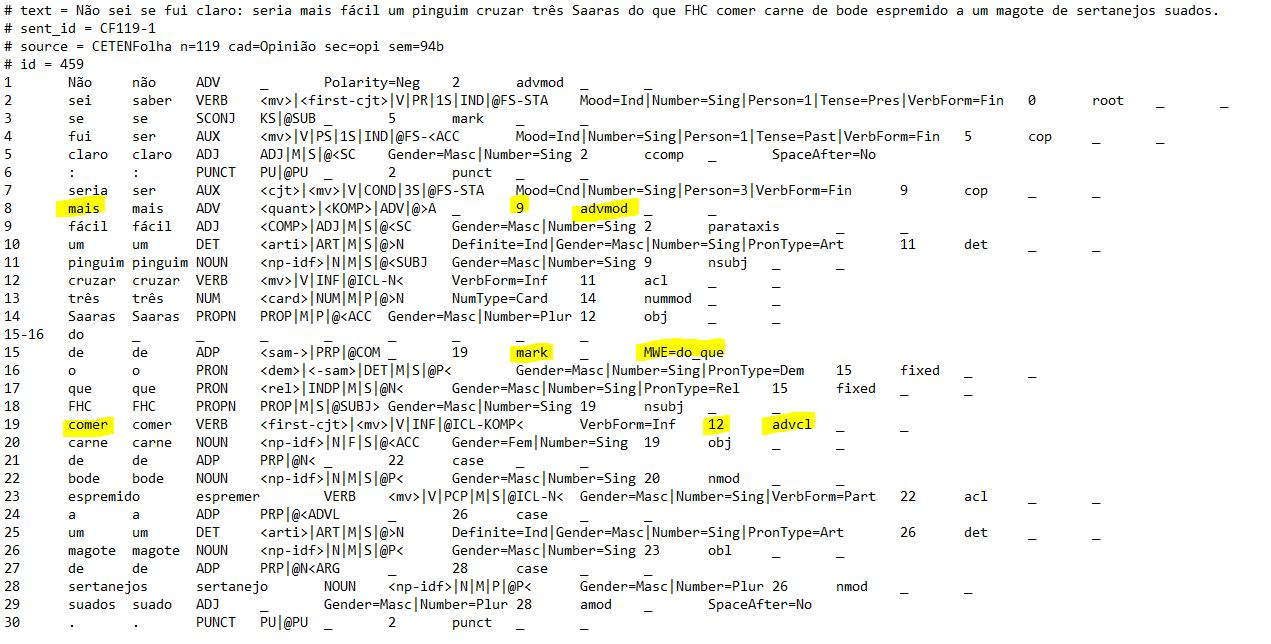
\includegraphics[width=\textwidth,height=\textheight,keepaspectratio]{imagesDrive/image17.png}
	    \caption{Não sei se fui claro: seria \emph{mais} fácil um pinguim cruzar três Saaras \emph{do que} FHC comer carne de bode espremido a um magote de sertanejos suados.}
	    \label{fig:comparative5}
	\end{figure}{}

	\begin{figure}[H]
	    \centering
	    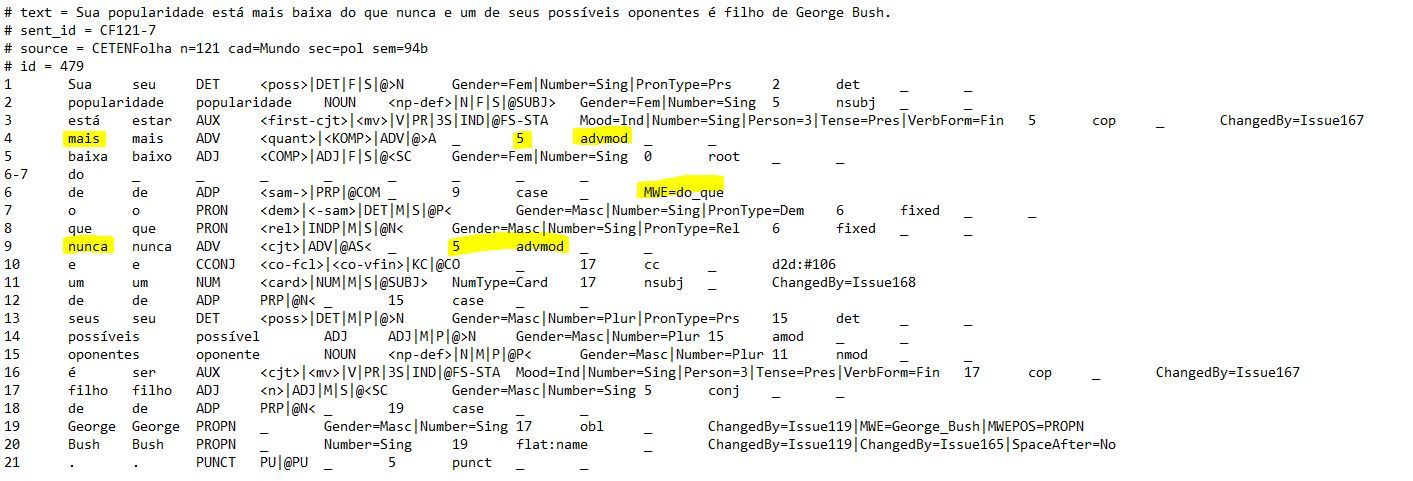
\includegraphics[width=\textwidth,height=\textheight,keepaspectratio]{imagesDrive/image40.png}
	    \caption{Sua popularidade está \emph{mais} baixa \emph{do que} nunca e um de seus possíveis oponentes é filho de George Bush.}
	    \label{fig:comparative6}
	\end{figure}{}

	\subsection{menos do que}

	\fullref{fig:comparative7}

	\fullref{fig:comparative8}

	\begin{figure}[H]
	    \centering
	    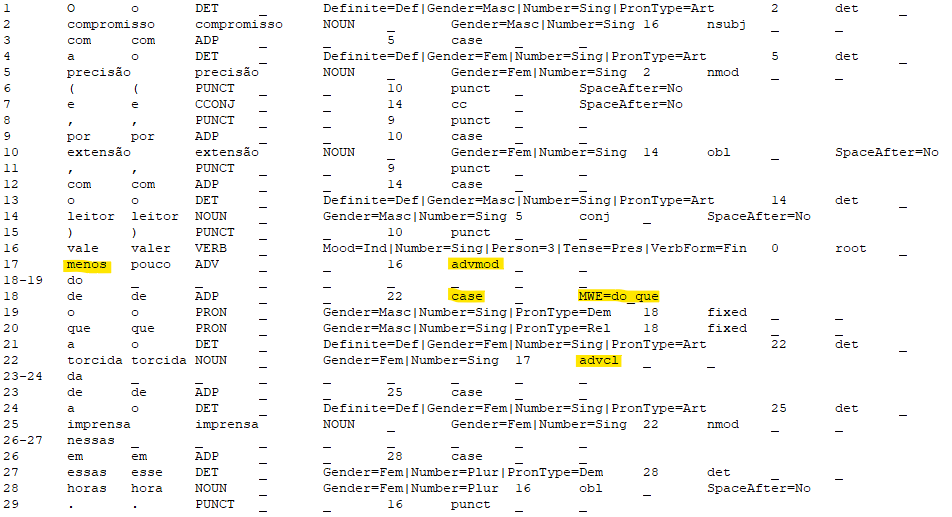
\includegraphics[width=\textwidth,height=\textheight,keepaspectratio]{imagesDrive/comparativo1.png}
	    \caption{O compromisso com a precisão (e, por extensão, com o leitor) vale \emph{menos do que} a torcida da imprensa nessas horas.}
	    \label{fig:comparative7}
	\end{figure}{}

	\begin{figure}[H]
	    \centering
	    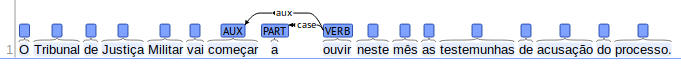
\includegraphics[width=\textwidth,height=\textheight,keepaspectratio]{imagesDrive/image43.png}
	    \caption{Segundo explicou o dirigente José Azevedo, a entrada em vigor dos novos diplomas trouxe consigo «inúmeras anomalias, geradoras de injustiças gritantes», como é o caso dos profissionais que, depois de subirem na carreira, ficam a ganhar \emph{menos do que} antes da progressão.}
	    \label{fig:comparative8}
	\end{figure}{}

	\subsection{melhor do que}

	\fullref{fig:comparative9}

	\fullref{fig:comparative10}

	\begin{figure}[H]
	    \centering
	    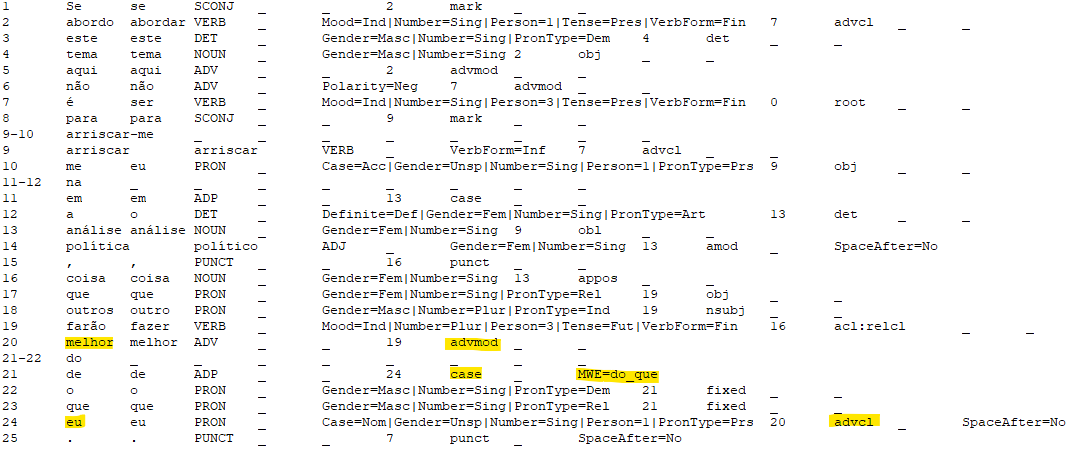
\includegraphics[width=\textwidth,height=\textheight,keepaspectratio]{imagesDrive/comparativo2.png}
	    \caption{Se abordo este tema aqui não é para arriscar-me na análise política, coisa que outros farão \emph{melhor do que} eu.}
	    \label{fig:comparative9}
	\end{figure}{}

	\begin{figure}[H]
	    \centering
	    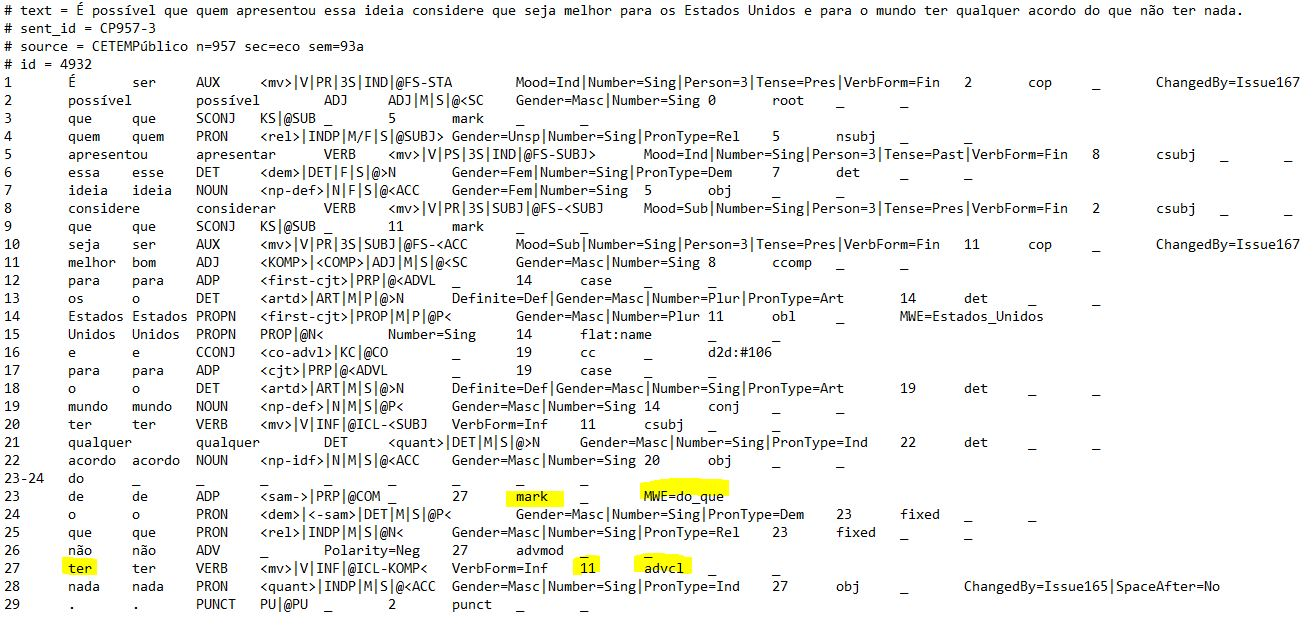
\includegraphics[width=\textwidth,height=\textheight,keepaspectratio]{imagesDrive/image54.png}
	    \caption{É possível que quem apresentou essa ideia considere que seja \emph{melhor} para os Estados Unidos e para o mundo ter qualquer acordo \emph{do que} não ter nada.}
	    \label{fig:comparative10}
	\end{figure}{}

	\subsection{pior do que}

	\fullref{fig:comparative11}

	\begin{figure}[H]
	    \centering
	    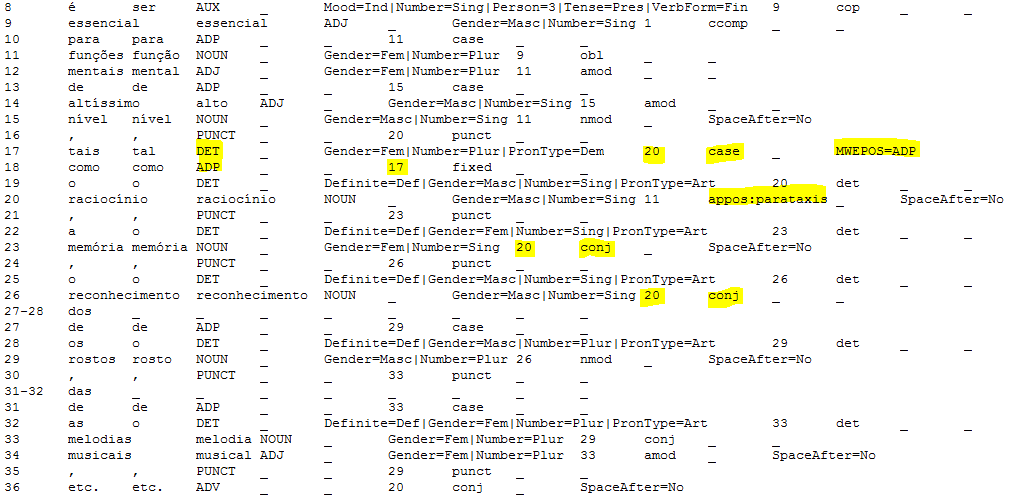
\includegraphics[width=\textwidth,height=\textheight,keepaspectratio]{imagesDrive/image18.png}
	    \caption{Eurico e Milton Areal porque o terreno estava quase impraticável, mas nem melhor nem \emph{pior do que} na primeira metade do encontro e o Tirsense parecia mais fresco e estava em situação de vantagem numérica.}
	    \label{fig:comparative11}
	\end{figure}{}


	\subsection{tão/tanto quanto}

	\fullref{fig:comparative12}

	\fullref{fig:comparative13}

	\fullref{fig:comparative14}

	\fullref{fig:tantoquanto}

	\begin{figure}[H]
	    \centering
	    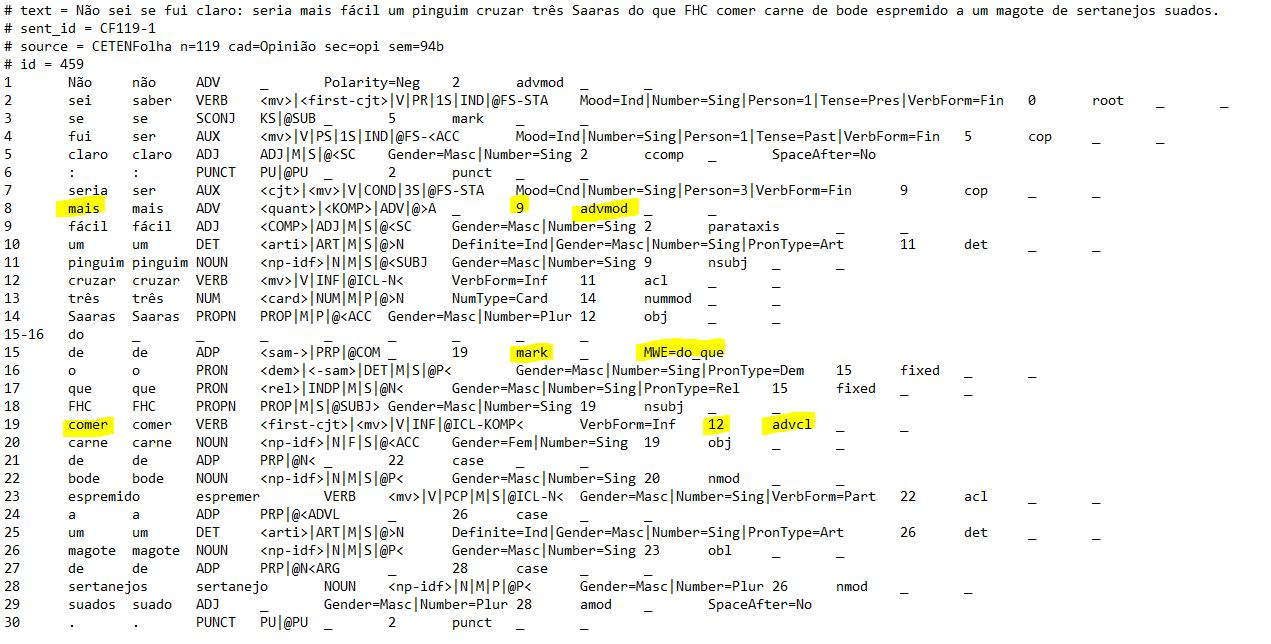
\includegraphics[width=\textwidth,height=\textheight,keepaspectratio]{imagesDrive/image15.png}
	    \caption{Hopkins diz que, ao contrário dos seus filmes anteriores, que «eram \emph{tão} divertidos \emph{quanto} ver tinta a secar» e «bons exercícios de disciplina e economia e tudo isso», este é um filme do tipo que lhe apetece fazer agora -- acção.}
	    \label{fig:comparative12}
	\end{figure}{}

	\begin{figure}[H]
	    \centering
	    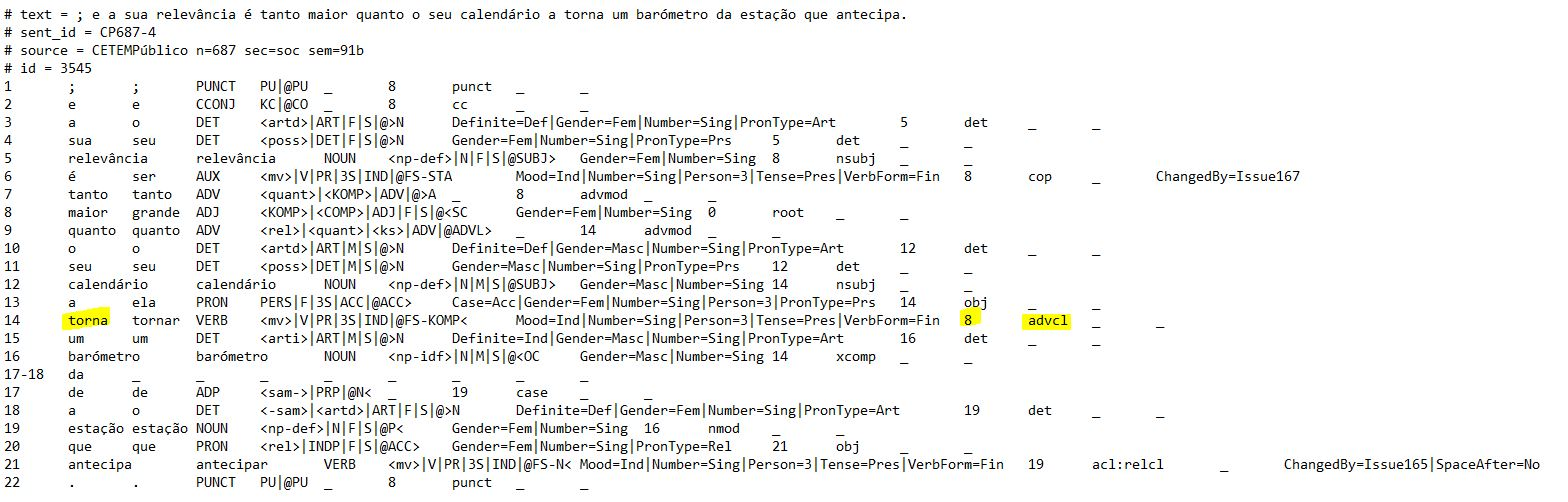
\includegraphics[width=\textwidth,height=\textheight,keepaspectratio]{imagesDrive/image13.png}
	    \caption{; e a sua relevância é \emph{tanto} maior \emph{quanto} o seu calendário a torna um barómetro da estação que antecipa.}
	    \label{fig:comparative13}
	\end{figure}{}

	\begin{figure}[H]
	    \centering
	    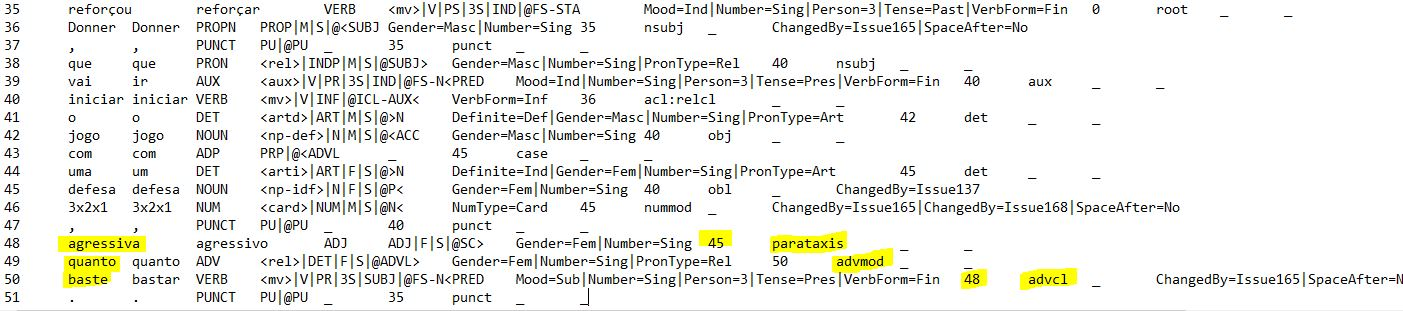
\includegraphics[width=\textwidth,height=\textheight,keepaspectratio]{imagesDrive/image5.png}
	    \caption{Nestes últimos dias, os bracarenses apenas têm estudado «pormenores do jogo, pois, quando duas equipas de nível semelhante se encontram, os pormenores é que decidem», reforçou Donner, que vai iniciar o jogo com uma defesa 3x2x1, agressiva \emph{quanto} baste.}
	    \label{fig:comparative14}
	\end{figure}{}

	\begin{figure}[H]
	    \centering
	    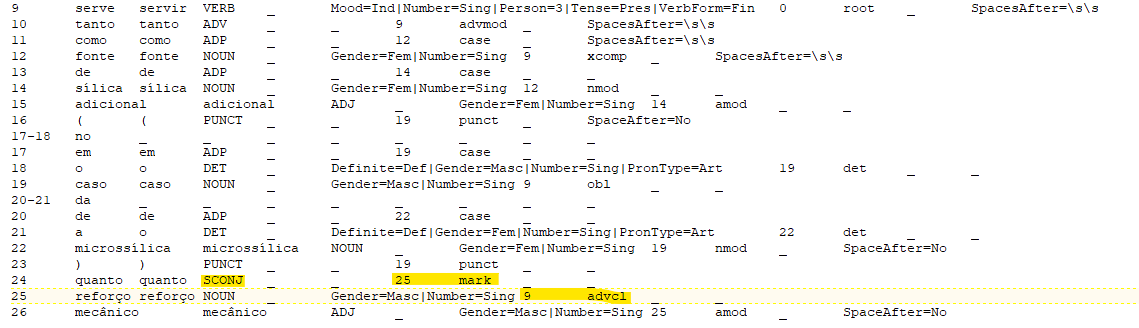
\includegraphics[width=\textwidth,height=\textheight,keepaspectratio]{imagesDrive/tantoquanto.png}
	    \caption{serve \emph{tanto} como fonte de silica adicional (no caso da microssilica)\emph{ quanto reforço} mecânico}
	    \label{fig:tantoquanto}
	\end{figure}{}

	\section{Elementos discursivos}

	\subsection{É que}\label{sec:eque}

	A construção \say{é que} pode aparecer de duas maneiras: marcada ou não como MWE. Como MWE, \say{é que} é uma ocorrência típica do discurso oral, sem ligação clara com a estrutura da oração. Por outro lado, \say{é} e \say{que} são independentes entre si quando introduzem uma oração subordinada substantiva predicativa ou subjetiva.

	Quando \say{é que} tem esse efeito discursivo, anota-se da seguinte maneira:

		É: tem upos \emph{AUX} e deprel \emph{discourse}, e aponta para a head da oração; 

		Que: tem upos \emph{SCONJ} e deprel \emph{fixed}, e aponta para \say{é}. \newline

		\fullref{dep:equeMWE1}

		\fullref{fig:equeMWE2}

		\fullref{fig:equeMWE3} \newline

	Igualmente, consideramos \say{Não é que} como MWE.  

	\say{\emph{Não é que} o sábio das matrizes encontrou, no PSD, entusiastas seguidores?} 


		\begin{figure}[H]
			\centering
			\vspace{.8cm}
			\begin{dependency}
				\begin{deptext}
					ADV \& ADV \& AUX \& SCONJ \& VERB \& DET \& NOUN \& SCONJ \& VERB \& DET \& NOUN \\
					Só \& depois \& é \& que \& levanto \& a \& cabeça \& para \& fazer \& um \& lançamento \\
					só \& depois \& ser \& que \& levantar \& o \& cabeça \& para \& fazer \& um \& lançamento \\
				\end{deptext}
				\depedge{2}{1}{advmod}
				\depedge{5}{2}{advmod}
				\depedge{5}{3}{discourse}
				\depedge{3}{4}{fixed}
				\deproot{5}{root}
				\depedge{7}{6}{det}
				\depedge{5}{7}{obj}
				\depedge{9}{8}{mark}
				\depedge{5}{9}{advcl}
				\depedge{11}{10}{det}
				\depedge{9}{11}{obj}
			\end{dependency}
			\caption{Só depois \emph{é que} levanto a cabeça para fazer um lançamento}
			\label{dep:equeMWE1}
		\end{figure}

	\begin{figure}[H]
    	\centering
    	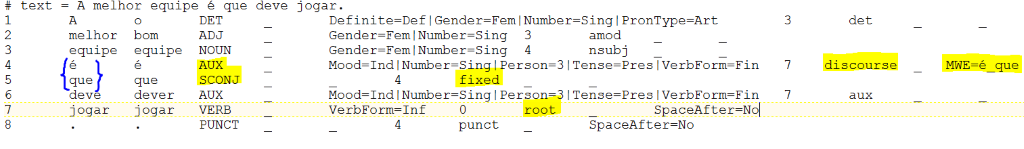
\includegraphics[width=\textwidth,height=\textheight,keepaspectratio]{imagesDrive/image16.png}
    	\caption{A melhor equipe \emph{é que} deve jogar}
    	\label{fig:equeMWE2}
    	\end{figure}{}

	\begin{figure}[H]
    	\centering
    	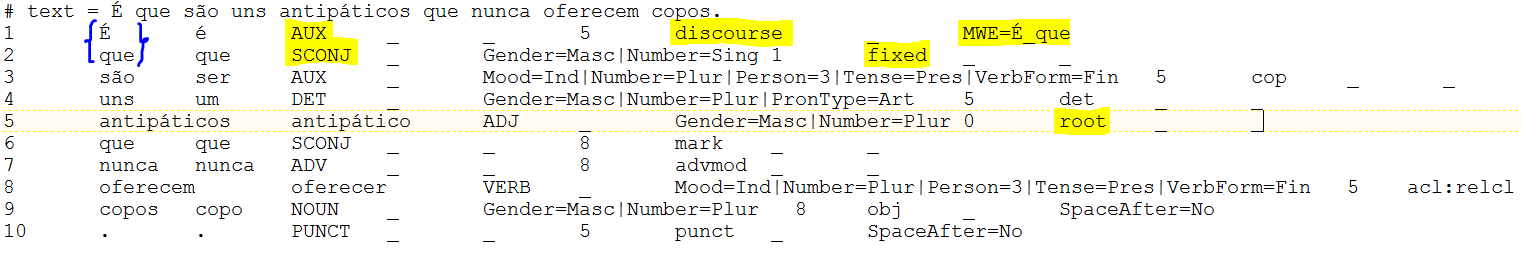
\includegraphics[width=\textwidth,height=\textheight,keepaspectratio]{imagesDrive/image71.png}
    	\caption{\emph{É que} são uns antipáticos que nunca oferecem copos}
    	\label{fig:equeMWE3}
    	\end{figure}{}

	Quando \say{é} e \say{que} são independentes, eles não formam MWE e podem se encaixar em uma das situações a seguir:

	\begin{enumerate}
		\item A conjunção subordinativa (\emph{SCONJ}) introduz uma oração subordinada substantiva predicativa, cujo núcleo tem deprel \emph{ccomp}. O verbo \say{ser} é pleno (\emph{VERB/root}), e o nome que o precede tem deprel \emph{nsubj}.

		\fullref{fig:equesemMWE1}

		\fullref{fig:equesemMWE3}		

		Decidimos que ocorrências como \say{o bom}, \say{o pior}, \say{o espantoso} ou \say{o certo} seriam marcadas como \emph{DET NOUN}, de modo análogo a frases como \say{A desgraça é que...}. Isso facilita que classifiquemos o adjetivo, que aqui se comporta como substantivo, como \emph{nsubj} da oração. (Ver \fullref{fig:equesemMWE2})

		\begin{figure}[H]
	    	\centering
	    	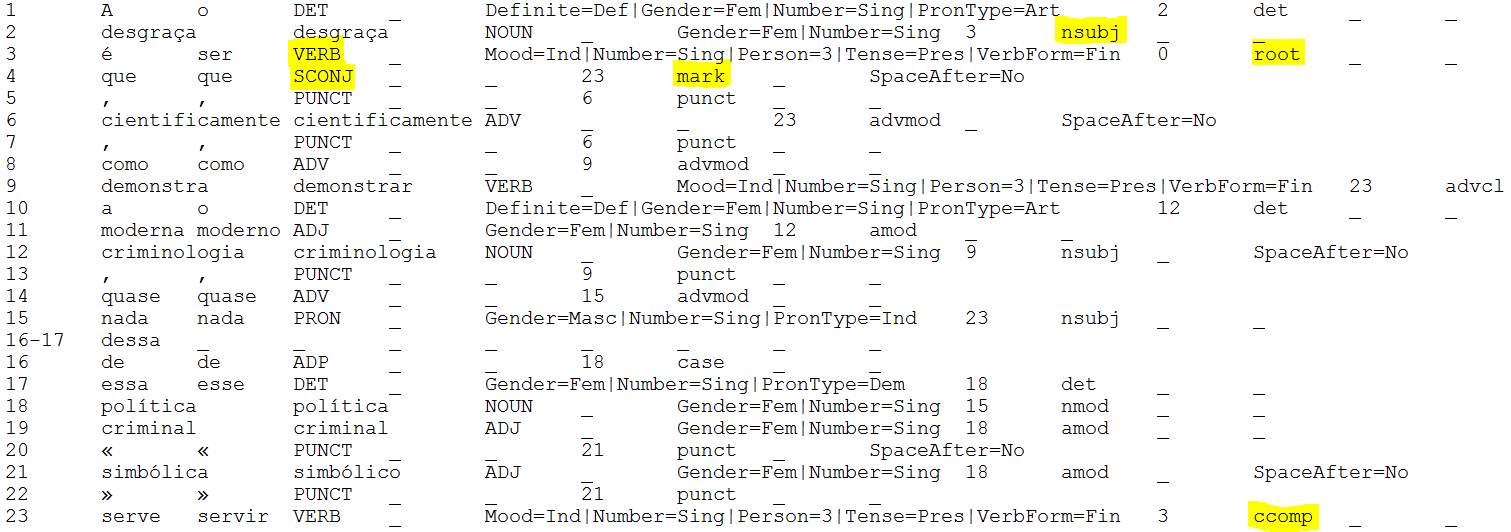
\includegraphics[width=\textwidth,height=\textheight,keepaspectratio]{imagesDrive/image21.png}
	    	\caption{A desgraça é que, cientificamente, como demonstra a moderna criminologia, quase nada dessa política criminal «simbólica» serve para atenuar o gravíssimo problema da criminalidade.}
	    	\label{fig:equesemMWE1}
	    	\end{figure}{}

		\begin{figure}[H]
	    	\centering
	    	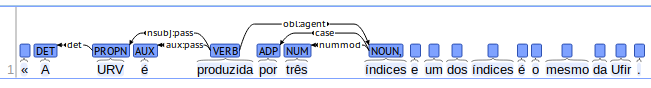
\includegraphics[width=\textwidth,height=\textheight,keepaspectratio]{imagesDrive/image59.png}
	    	\caption{O bom é que o Fernando Henrique não estava presente}
	    	\label{fig:equesemMWE2}
	    	\end{figure}{}

		\begin{figure}[H]
	    	\centering
	    	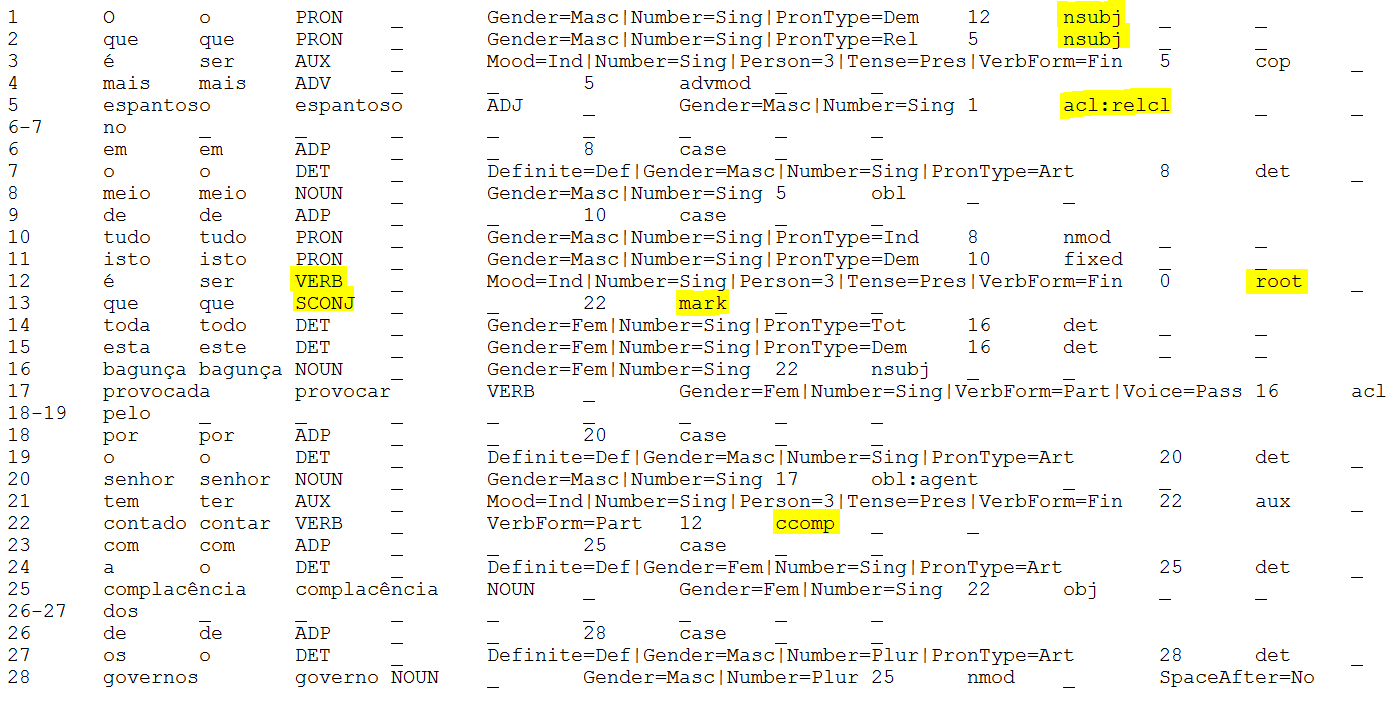
\includegraphics[width=\textwidth,height=\textheight,keepaspectratio]{imagesDrive/image56.png}
	    	\caption{O que é mais espantoso no meio de tudo isto é que toda esta bagunça provocada pelo senhor tem contado com a complacência dos governos}
	    	\label{fig:equesemMWE3}
	    	\end{figure}{}

		\item A conjunção subordinativa (\emph{SCONJ}) introduz uma oração subordinada substantiva subjetiva, cujo núcleo tem deprel \emph{csubj}. O verbo \say{ser} é \emph{AUX/cop}, e o adjetivo que o precede é \emph{root}.

		Na \fullref{fig:equesemMWE4}, por exemplo, ao substituirmos por \say{isso} a oração introduzida por \say{que} e a invertemos, temos \say{Isso é certo}. 

		\begin{figure}[H]
	    	\centering
	    	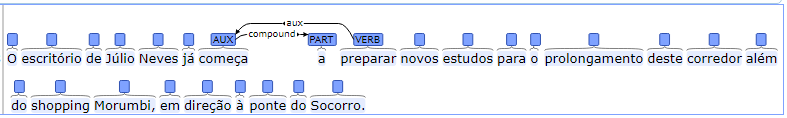
\includegraphics[width=\textwidth,height=\textheight,keepaspectratio]{imagesDrive/image26.png}
	    	\caption{Certo é que Pinochet fez do país uma casa portuguesa, com certeza}
	    	\label{fig:equesemMWE4}
	    	\end{figure}{}

	\end{enumerate}

		Mais casos difíceis:

		\fullref{fig:equedif1}: \say{é} foi anotado como AUX/discourse e \say{que} como SCONJ/mark. Não é um caso de MWE, visto que consideramos apenas \say{é} como discourse.

		\fullref{fig:equedif2}: \say{R} é \emph{root} e \say{é} tem deprel \emph{parataxis}.

		\fullref{fig:equedif3}

		\begin{figure}[H]
	    	\centering
	    	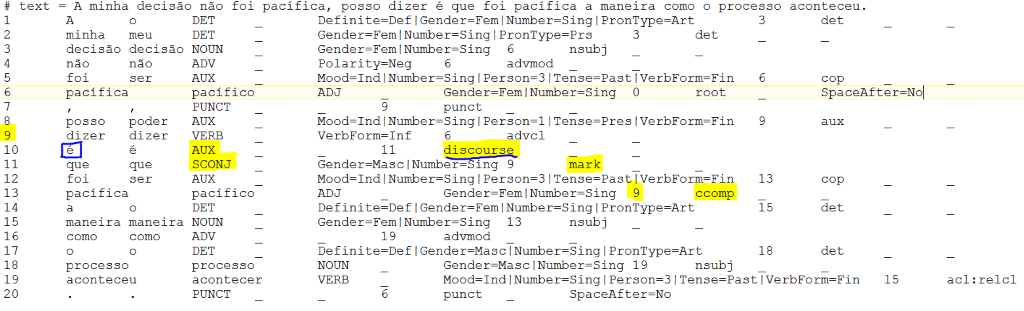
\includegraphics[width=\textwidth,height=\textheight,keepaspectratio]{imagesDrive/image45.png}
	    	\caption{A minha decisão não foi pacífica, posso dizer é que foi pacífica a maneira como o processo aconteceu}
	    	\label{fig:equedif1}
	    	\end{figure}{}

		\begin{figure}[H]
	    	\centering
	    	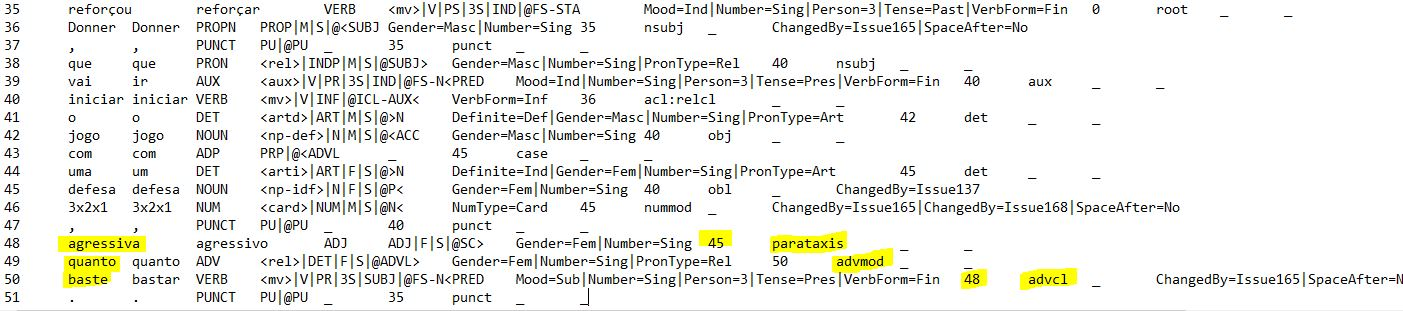
\includegraphics[width=\textwidth,height=\textheight,keepaspectratio]{imagesDrive/image6.png}
	    	\caption{R. -- Nestes casos, a boa política é que durma em casa}
	    	\label{fig:equedif2}
	    	\end{figure}{}

		\begin{figure}[H]
	    	\centering
	    	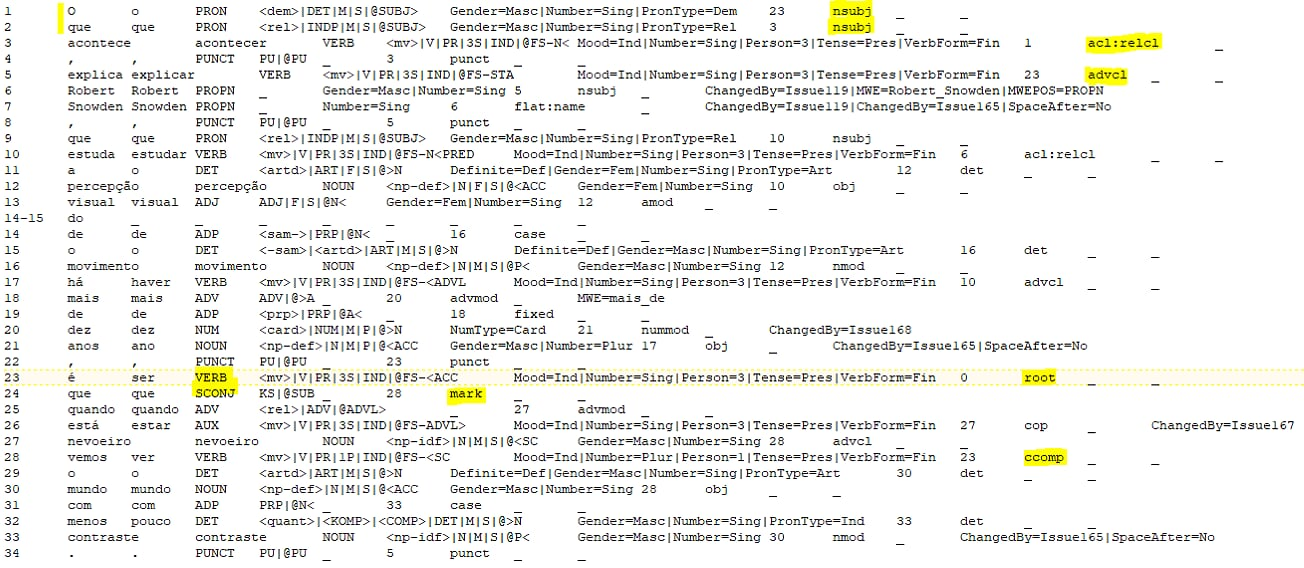
\includegraphics[width=\textwidth,height=\textheight,keepaspectratio]{imagesDrive/image64.png}
	    	\caption{O que acontece, explica Robert Snowden, que estuda a percepção visual do movimento há mais de dez anos, é que quando está nevoeiro vemos o mundo com menos contraste}
	    	\label{fig:equedif3}
	    	\end{figure}{}

	

	\subsection{Como / tal como}

		Existem dois casos em que a combinação \say{tal como} aparece. Em um deles, \say{tal como} é equivalente a \say{do mesmo modo que} ou \say{conforme}, como na \fullref{fig:talcomo1}.

		No outro caso, \say{tal como} indica uma espécie de hiperonímia, como na \fullref{fig:talcomo2}.

		\begin{figure}[H]
	    	\centering
	    	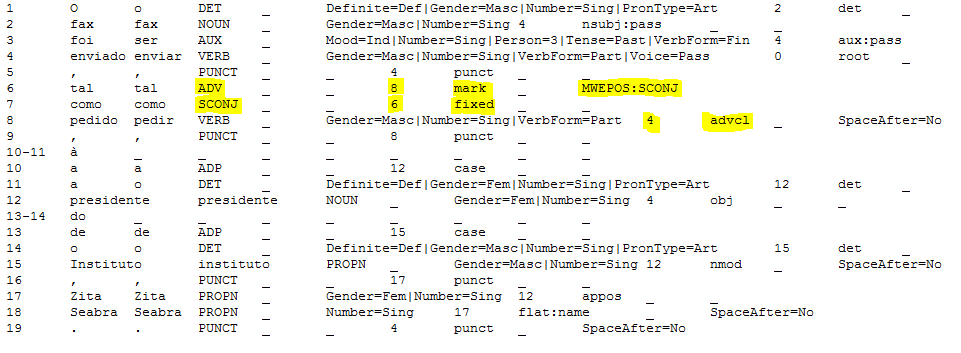
\includegraphics[width=\textwidth,height=\textheight,keepaspectratio]{imagesDrive/image36.png}
	    	\caption{O fax foi enviado, \emph{tal como} pedido, à presidente do Instituto, Zita Seabra.}
	    	\label{fig:talcomo1}
	    	\end{figure}{}
		
		\begin{figure}[H]
	    	\centering
	    	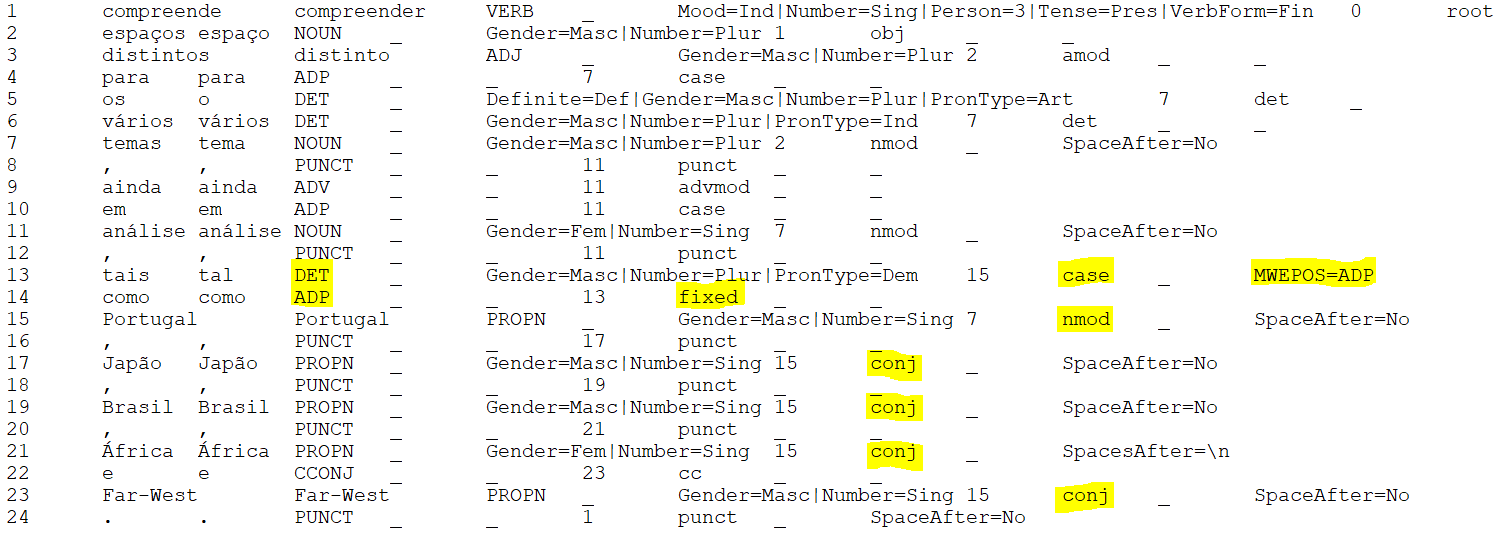
\includegraphics[width=\textwidth,height=\textheight,keepaspectratio]{imagesDrive/como2.png}
	    	\caption{A zona lúdica, com os divertimentos, áreas comerciais de «souvenirs» e de restauração, compreende espaços distintos para os vários temas, ainda em análise, \emph{tais como} Portugal, Japão, Brasil, África e Far-West.}
	    	\label{fig:talcomo2}
	    	\end{figure}{}

		Para solucionarmos essa diferença, criamos dois tipos distintos de MWE (expressão multipalavra). Nos casos do primeiro tipo, em que há equivalência com \say{conforme}, \say{tal como} foi anotado como MWE com valor de conjunção subordinativa. 

		Essa MWE com valor de conjunção subordinativa inicia uma oração adverbial; logo, o núcleo do fragmento, independente de ser verbo ou não, teve deprel anotado como \emph{advcl}. (\fullref{fig:talcomo3})

		\begin{figure}[H]
	    	\centering
	    	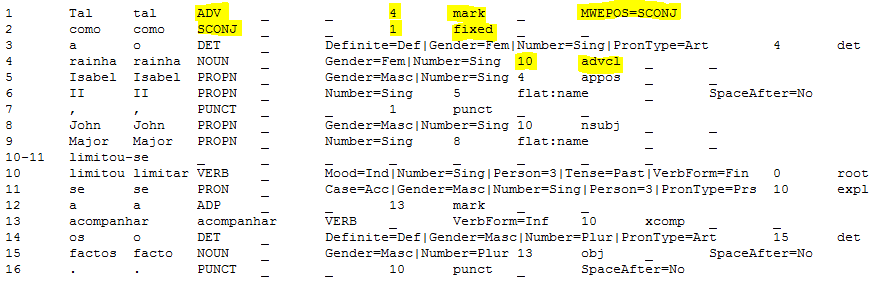
\includegraphics[width=\textwidth,height=\textheight,keepaspectratio]{imagesDrive/image69.png}
	    	\caption{\emph{Tal como} a rainha Isabel II, John Major limitou-se a acompanhar os factos.}
	    	\label{fig:talcomo3}
	    	\end{figure}{}

		Para os casos em que \say{tal como} indica hiperonímia, criamos uma MWE com valor prepositivo (\fullref{fig:talcomo2}).

		Além disso, essa estrutura de hiperonímia também pode aparecer em frases com apenas \say{como}, em vez de \say{tal como}. Essas frases, em termos semânticos, têm valores semelhantes; no entanto, não há MWE nas frases de \say{como} (\fullref{fig:talcomo4}).

		\begin{figure}[H]
	    	\centering
	    	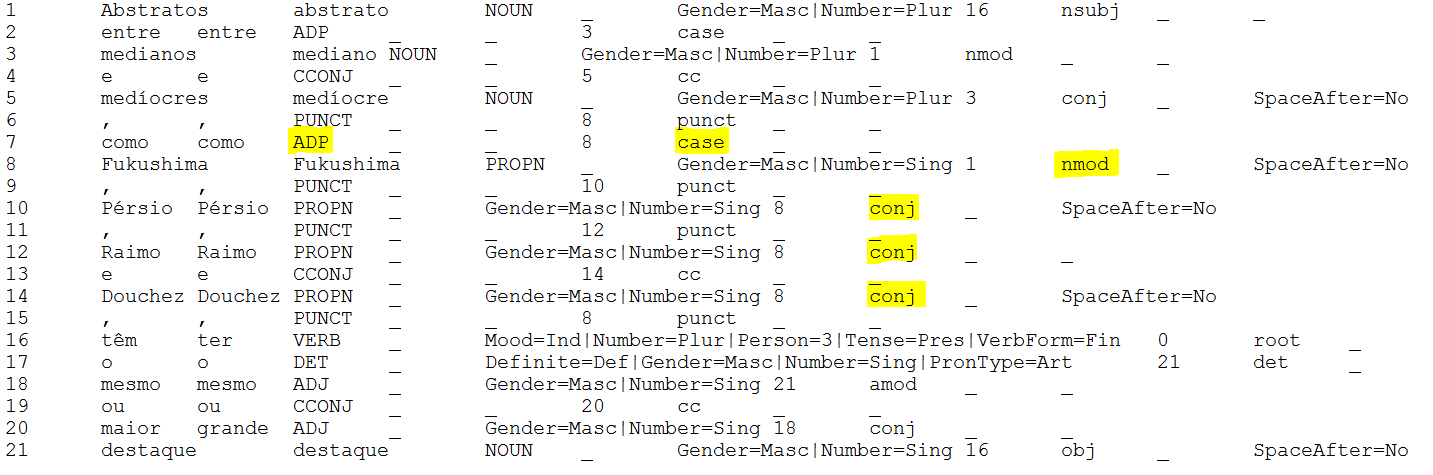
\includegraphics[width=\textwidth,height=\textheight,keepaspectratio]{imagesDrive/como1.png}
	    	\caption{Abstratos entre medianos e medíocres, \emph{como} Fukushima, Pérsio, Raimo e Douchez, têm o mesmo ou maior destaque que Volpi e nada que se possa chamar de autonomia para oferecer como lenitivo.}
	    	\label{fig:talcomo4}
	    	\end{figure}{}

	\section{O que fazer com...}\label{sec:quefazer}

		\subsection{Endereços de internet, e-mails etc.}
		
			Endereços de internet, e-mails etc. são anotados como \emph{NOUN}. Com relação à função sintática, em geral estarão envolvidos em estrutura de aposto (Ver \fullref{sec:aposto}).

		\subsection{Enumerações, porcentagens e parênteses}

			\fullref{fig:epp}

			\begin{figure}[H]
				\centering
				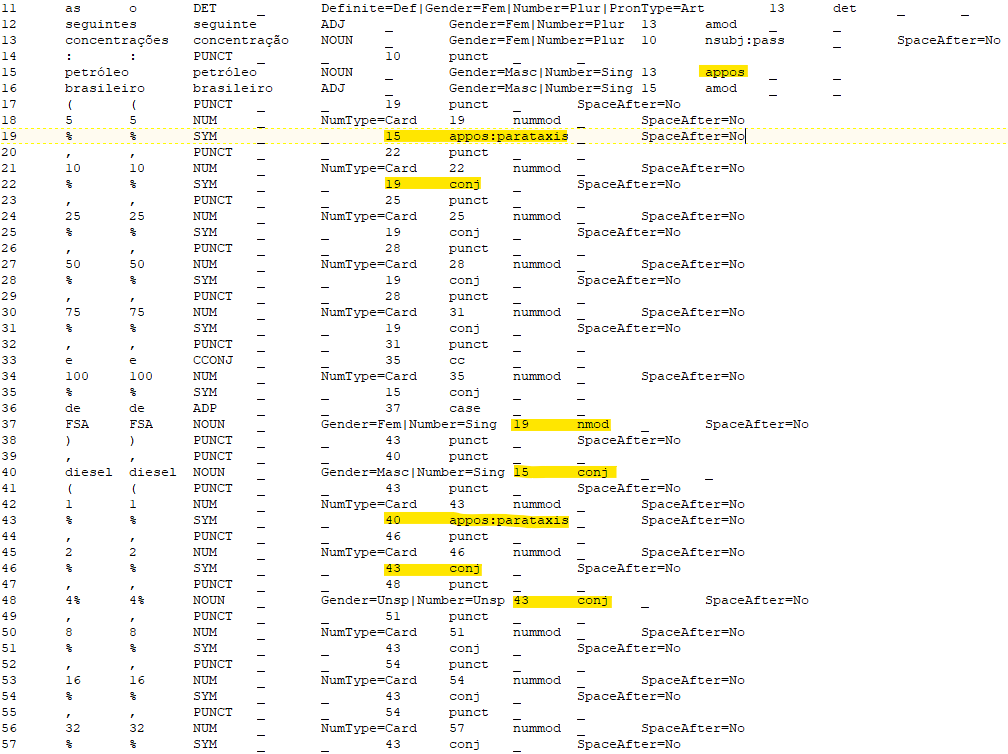
\includegraphics[width=\textwidth,height=\textheight,keepaspectratio]{imagesDrive/epp.png}
				\caption{as seguintes concentrações: petróleo brasileiro (5\%, 10\%, 25\%, 50\%, 75\%, e 100\% de FSA), diesel (1\%, 2\%, 4\%, 8\%, 16\%, 32\%, e 64\% de FSA) e gasolina (1\%, 2,5\%, 5\%, 10\%, e 20\% de FSA)}
				\label{fig:epp}
			\end{figure}{}

		\subsection{Nome seguido de nome: \emph{appos}, \emph{compound}, \emph{flat:name} ou \emph{nmod/amod}?}\label{sec:nomeseguidodenome}

			Substantivos (\emph{NOUN}) e nomes próprios (\emph{PROPN}) seguidos de outros substantivos ou nomes próprios podem receber diferentes funções sintáticas.


			\subsubsection{\emph{appos}}\label{sec:nomeappos}

				Utilizado quando o segundo nome especifica um tipo do primeiro nome
	
				grupos \emph{éter}
	
				cepa \emph{Pseudomonas}
	
				sistemas \emph{metano-éster}
	
				base \emph{éster}
	
				base \emph{água}
	
				razão \emph{ar/combustível }
	
				combustão \emph{in-situ}
	
				metais \emph{prata}, lítio e cobre
	
				ânion \emph{oxigênio}
	
				ácido \emph{p-tolueno}
	
				Decreto \emph{n.º 5.297}
	
				Lei \emph{nº 997} (os algarismos também são \emph{appos} de \say{nº})
	
				íons \emph{carbonato}
	
				tipo \emph{FPSO}
	
				campo \emph{onshore}
	
				corrente \emph{infra-estrutura}
	
				fácie \emph{silte}
	
				portal \emph{http://www.lei.furg.br/sidipla}
	
				Figura \emph{1}
	
				Figura \emph{2}
	
				Figura \emph{3}
	
				variáveis \emph{concentração} de inóculo, temperatura e teor de umidade inicial
	
				enzima \emph{cloroperoxidase}
	
				tipo \emph{ramnolipídeo}
	
				fator \emph{probabilidade} de crescimento
	
				Bacia \emph{Pelotas}
	
				Goma \emph{Xantana}

				Ver também: \fullref{sec:aposto}

			\subsubsection{\emph{compound}}\label{sec:nomecompound}

				Utilizado quando a expressão inteira é um termo relevante para algum domínio; expressão cristalizada, possivelmente com flexão interna

				Odontesthes \emph{argentinensis}
	
				Clupea \emph{arengus}
	
				efeito \emph{estufa}
	
				meio \emph{ambiente}
	
				Pseudomonas \emph{aeruginosa}
	
				dimetil \emph{éter}
	
				grupo \emph{controle}
	
				desvio \emph{padrão}
	
				Gás \emph{Natural}
	
				Gás \emph{Natural Liquefeito}
	
				Inversão \emph{Magnética Compacta Generalizada}
	
				Sistema de \emph{Informação} Geográfica
	
				Engenharia \emph{Química}

				Ver também: \fullref{sec:mwe}

			\subsubsection{\emph{flat:name}}\label{sec:nomeflatname}

				Utilizado quando é nome de empresa/pessoa; sem sintaxe interna

				Baleia \emph{Franca}
	
				Corrente \emph{Malvinas}
	
				Cone \emph{do Rio Grande}
	
				Alto \emph{de Cabo Frio}
	
				Petróleo \emph{Brasileiro}
	
				Java \emph{Climate}
	
				Wind \emph{Down}
	
				Doris \emph{Engenharia}
	
				Safe \emph{Drinking Water Act}
	
				Occupational \emph{safety}
	
				Molten \emph{carbonate}
	
				Santa \emph{Marta}
	
				XXXX \emph{et al.}
	
				São \emph{Paulo}
	
				Solvay \emph{Solexis}
	
				American \emph{Petroleum Institute}
	
				International \emph{Energy Agency}
	
				Sir \emph{William Grove}
	
				Radix \emph{Engenharia}
	
				Thiago \emph{Cleyandson}
	
				Estados \emph{Unidos}
	
				Dow \emph{Chemicals}
	
				Espírito \emph{Santo}
	
				proton \emph{exchange}
	
				Exxon \emph{Valdez}
	
				Aspen \emph{Plus}
	
				two-step \emph{sintering}
	
				Ver também: \fullref{sec:mwe}

			\subsubsection{\emph{nmod} e \emph{amod}}

				São utilizados quando não se aplicam os casos anteriores; no caso de substantivo (\emph{nmod}), há a preposição \say{de} ou ela está omitida

				emulsões \emph{base} éster (\say{éster} é \emph{appos} de \say{base})
	
				navio \emph{tipo} A (\say{A} é \emph{appos} de \say{tipo})
	
				Ver também: \fullref{sec:adjuntoadnominal}
				
				
		\subsection{Referências bibliográficas, figuras e tabelas}	
			
			As referências bibliográficas que ocorrem no fim de uma frase são filhas do \emph{root} da sentença e recebem deprel \emph{parataxis}, conforme a \fullref{fig:refbibliofinal}. Ver também: \fullref{sec:nomeflatname}.
			
				\begin{figure}[H]
				    	\centering
				    	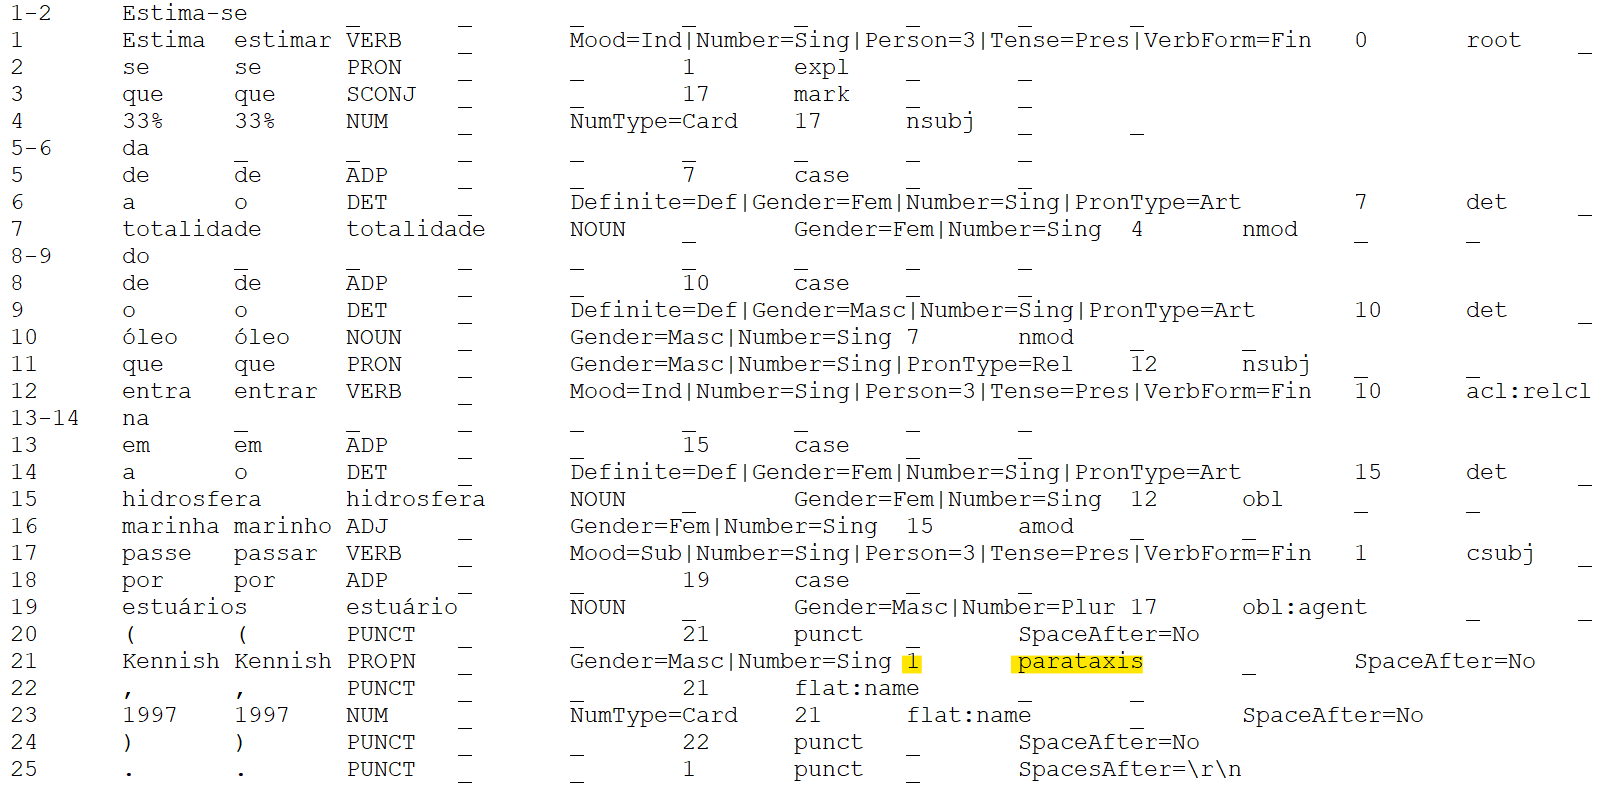
\includegraphics[width=\textwidth,height=\textheight,keepaspectratio]{imagesDrive/refbibliofinal2.png}
				    	\caption{Estima-se que 33\% da totalidade do óleo que entra na hidrosfera marinha passe por estuários (\emph{Kennish, 1997}).}
				    	\label{fig:refbibliofinal}
				    	\end{figure}{}
			
			Do mesmo modo, as menções a figuras e tabelas, independentemente da posição na frase, são filhas do \emph{root} da sentença e recebem deprel \emph{parataxis}: \fullref{fig:reffigura}. Ver também: \fullref{sec:nomeappos}.
			
				\begin{figure}[H]
					    	\centering
					    	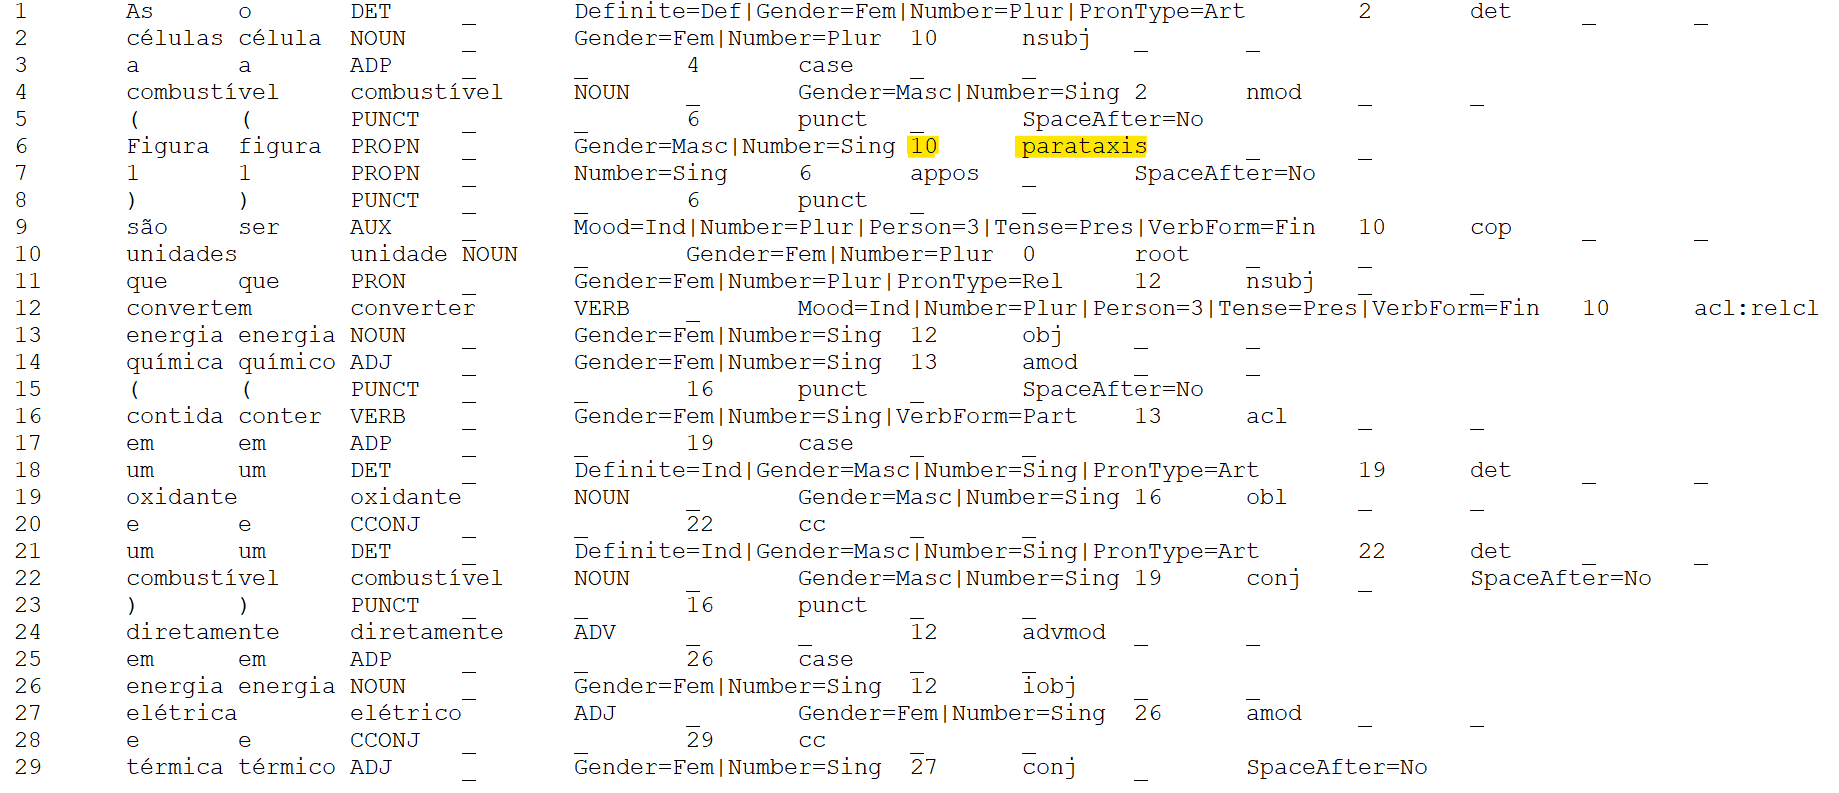
\includegraphics[width=\textwidth,height=\textheight,keepaspectratio]{imagesDrive/reffigura2.png}
					    	\caption{As células a combustível (\emph{Figura} 1) são unidades que convertem energia química (contida em um oxidante e um combustível) diretamente em energia elétrica e térmica}
					    	\label{fig:reffigura}
					    	\end{figure}{}

\chapter{Apêndice}

	\hyperlink{toc}{Ir para tabela de conteúdos\\}

	Todas as listas são retiradas do corpus Bosque-UD em sua versão 2.5.
	
	\begin{table}[]
		\centering
		\begin{tabular}{|c|c|}
			\hline
			\textbf{Verbo de ligação} & \textbf{Frequência} \\\hline
			estar & 33\\\hline
			ser & 105\\\hline
		\end{tabular}
		\caption{Lista das 2 palavras que ocorrem 138 vezes como verbo de ligação (\emph{AUX/cop}) no Bosque-UD}
		\label{tab:verbosdeligacao}
	\end{table}

	\begin{table}[]
		\centering
		\begin{tabular}{|c|c|}
			\hline
			\textbf{Voz passiva} & \textbf{Frequência} \\\hline
			ter & 465\\\hline
			ir & 341\\\hline
			estar & 126\\\hline
			ser & 48\\\hline
			haver & 36\\\hline
		\end{tabular}
		\caption{Lista das 5 palavras que ocorrem 1016 vezes como locução verbal de tempo composto (\emph{AUX/aux}) no Bosque-UD}
		\label{tab:loctempocomposto}
	\end{table}

	\begin{longtable}{ p{3cm} | p{1cm} | p{3cm} | p{1cm} }
		\hline
		\textbf{Primeiro verbo (ordem alfabética)} & \textbf{\#} & \textbf{Primeiro verbo (ordem de frequência)} & \textbf{\#} \\\hline
		abster & 2 & poder & 398\\\hline
		acabar & 60 & dever & 221\\\hline
		aceder & 1 & estar & 130\\\hline
		aceitar & 6 & querer & 108\\\hline
		achar & 5 & ter & 86\\\hline
		aconselhar & 5 & conseguir & 83\\\hline
		acreditar & 2 & vir & 71\\\hline
		acusar & 30 & continuar & 64\\\hline
		admitir & 12 & tentar & 64\\\hline
		afirmar & 13 & começar & 63\\\hline
		aguentar & 1 & acabar & 60\\\hline
		ajudar & 9 & deixar & 51\\\hline
		alegar & 3 & fazer & 45\\\hline
		ambicionar & 1 & passar & 44\\\hline
		ameaçar & 15 & voltar & 41\\\hline
		andar & 6 & pretender & 39\\\hline
		anunciar & 2 & permitir & 37\\\hline
		aperceber & 1 & decidir & 33\\\hline
		apetecer & 1 & acusar & 30\\\hline
		aplicar & 1 & parecer & 22\\\hline
		apostar & 1 & procurar & 22\\\hline
		aprender & 5 & ficar & 21\\\hline
		apresentar & 2 & ser & 21\\\hline
		apressar & 1 & chegar & 20\\\hline
		aprestar & 1 & levar & 20\\\hline
		aproveitar & 1 & ver & 19\\\hline
		arriscar & 2 & dar & 18\\\hline
		atender & 1 & gostar & 17\\\hline
		atrever & 1 & obrigar & 17\\\hline
		autorizar & 3 & saber & 16\\\hline
		avisar & 1 & ameaçar & 15\\\hline
		bastar & 3 & precisar & 14\\\hline
		caber & 1 & preferir & 14\\\hline
		cansar & 1 & resolver & 14\\\hline
		cessar & 1 & afirmar & 13\\\hline
		chamar & 4 & admitir & 12\\\hline
		chegar & 20 & considerar & 12\\\hline
		citar & 1 & encontrar & 12\\\hline
		começar & 63 & dizer & 11\\\hline
		comprometer & 7 & costumar & 10\\\hline
		concordar & 3 & destinar & 10\\\hline
		condenar & 1 & limitar & 10\\\hline
		conduzir & 1 & ajudar & 9\\\hline
		confidenciar & 1 & esperar & 9\\\hline
		confirmar & 1 & preparar & 9\\\hline
		conseguir & 83 & pensar & 8\\\hline
		considerar & 12 & comprometer & 7\\\hline
		consistir & 7 & consistir & 7\\\hline
		consultar & 1 & convidar & 7\\\hline
		contar & 1 & recusar & 7\\\hline
		continuar & 64 & aceitar & 6\\\hline
		contribuir & 3 & andar & 6\\\hline
		convencer & 6 & convencer & 6\\\hline
		convencionar & 1 & ir & 6\\\hline
		convidar & 7 & manter & 6\\\hline
		costumar & 10 & prometer & 6\\\hline
		credenciar & 1 & achar & 5\\\hline
		criticar & 1 & aconselhar & 5\\\hline
		culpar & 1 & aprender & 5\\\hline
		dar & 18 & forçar & 5\\\hline
		decidir & 33 & mandar & 5\\\hline
		declarar & 3 & parar & 5\\\hline
		declinar & 1 & propor & 5\\\hline
		dedicar & 2 & tender & 5\\\hline
		deixar & 51 & visar & 5\\\hline
		depender & 1 & chamar & 4\\\hline
		desafiar & 2 & desejar & 4\\\hline
		desejar & 4 & encarregar & 4\\\hline
		desistir & 1 & evitar & 4\\\hline
		destinar & 10 & haver & 4\\\hline
		dever & 221 & impedir & 4\\\hline
		dispor & 3 & interessar & 4\\\hline
		dizer & 11 & proibir & 4\\\hline
		duvidar & 1 & reconhecer & 4\\\hline
		empenhar & 2 & sentir & 4\\\hline
		encarregar & 4 & tencionar & 4\\\hline
		encontrar & 12 & tratar & 4\\\hline
		ensinar & 1 & alegar & 3\\\hline
		equivaler & 1 & autorizar & 3\\\hline
		escolher & 1 & bastar & 3\\\hline
		escusar & 2 & concordar & 3\\\hline
		esperar & 9 & contribuir & 3\\\hline
		estar & 130 & declarar & 3\\\hline
		estimar & 1 & dispor & 3\\\hline
		estimular & 1 & insistir & 3\\\hline
		estudar & 1 & optar & 3\\\hline
		evitar & 4 & ousar & 3\\\hline
		exigir & 1 & pôr & 3\\\hline
		exortar & 1 & abster & 2\\\hline
		experimentar & 1 & acreditar & 2\\\hline
		falar & 2 & anunciar & 2\\\hline
		faltar & 1 & apresentar & 2\\\hline
		fartar & 1 & arriscar & 2\\\hline
		fazer & 45 & dedicar & 2\\\hline
		ficar & 21 & desafiar & 2\\\hline
		fingir & 1 & empenhar & 2\\\hline
		foi & 1 & escusar & 2\\\hline
		forçar & 5 & falar & 2\\\hline
		garantir & 2 & garantir & 2\\\hline
		gostar & 17 & imaginar & 2\\\hline
		habituar & 1 & impor & 2\\\hline
		haver & 4 & importar & 2\\\hline
		imaginar & 2 & incentivar & 2\\\hline
		impedir & 4 & mostrar & 2\\\hline
		impor & 2 & necessitar & 2\\\hline
		importar & 2 & negar & 2\\\hline
		incentivar & 2 & ouvir & 2\\\hline
		incluir & 1 & queixar & 2\\\hline
		indagar & 1 & receber & 2\\\hline
		influenciar & 1 & referir & 2\\\hline
		informar & 1 & resistir & 2\\\hline
		insinuar & 1 & sentar & 2\\\hline
		insistir & 3 & tornar & 2\\\hline
		instar & 1 & aceder & 1\\\hline
		interessar & 4 & aguentar & 1\\\hline
		ir & 6 & ambicionar & 1\\\hline
		lembrar & 1 & aperceber & 1\\\hline
		levar & 20 & apetecer & 1\\\hline
		limitar & 10 & aplicar & 1\\\hline
		mandar & 5 & apostar & 1\\\hline
		manter & 6 & apressar & 1\\\hline
		merecer & 1 & aprestar & 1\\\hline
		mostrar & 2 & aproveitar & 1\\\hline
		necessitar & 2 & atender & 1\\\hline
		negar & 2 & atrever & 1\\\hline
		obrigar & 17 & avisar & 1\\\hline
		optar & 3 & caber & 1\\\hline
		orgulhar & 1 & cansar & 1\\\hline
		ousar & 3 & cessar & 1\\\hline
		ouvir & 2 & citar & 1\\\hline
		parar & 5 & condenar & 1\\\hline
		parecer & 22 & conduzir & 1\\\hline
		passado & 1 & confidenciar & 1\\\hline
		passar & 44 & confirmar & 1\\\hline
		pedir & 1 & consultar & 1\\\hline
		pensar & 8 & contar & 1\\\hline
		perder & 1 & convencionar & 1\\\hline
		permanecer & 1 & credenciar & 1\\\hline
		permitir & 37 & criticar & 1\\\hline
		persuadir & 1 & culpar & 1\\\hline
		planear & 1 & declinar & 1\\\hline
		poder & 398 & depender & 1\\\hline
		precisar & 14 & desistir & 1\\\hline
		preferir & 14 & duvidar & 1\\\hline
		preparar & 9 & ensinar & 1\\\hline
		pretender & 39 & equivaler & 1\\\hline
		prevenir & 1 & escolher & 1\\\hline
		prever & 1 & estimar & 1\\\hline
		procurar & 22 & estimular & 1\\\hline
		proibir & 4 & estudar & 1\\\hline
		projectar & 1 & exigir & 1\\\hline
		prometer & 6 & exortar & 1\\\hline
		propiciar & 1 & experimentar & 1\\\hline
		propor & 5 & faltar & 1\\\hline
		provocar & 1 & fartar & 1\\\hline
		pôr & 3 & fingir & 1\\\hline
		queixar & 2 & foi & 1\\\hline
		quer & 1 & habituar & 1\\\hline
		querer & 108 & incluir & 1\\\hline
		receber & 2 & indagar & 1\\\hline
		reclamar & 1 & influenciar & 1\\\hline
		recomeçar & 1 & informar & 1\\\hline
		recompensar & 1 & insinuar & 1\\\hline
		reconhecer & 4 & instar & 1\\\hline
		recordar & 1 & lembrar & 1\\\hline
		recusar & 7 & merecer & 1\\\hline
		reduzir & 1 & orgulhar & 1\\\hline
		referir & 2 & passado & 1\\\hline
		resistir & 2 & pedir & 1\\\hline
		resolver & 14 & perder & 1\\\hline
		respeitar & 1 & permanecer & 1\\\hline
		restar & 1 & persuadir & 1\\\hline
		retirar & 1 & planear & 1\\\hline
		saber & 16 & prevenir & 1\\\hline
		salientar & 1 & prever & 1\\\hline
		sentar & 2 & projectar & 1\\\hline
		sentir & 4 & propiciar & 1\\\hline
		ser & 21 & provocar & 1\\\hline
		soar & 1 & quer & 1\\\hline
		sonhar & 1 & reclamar & 1\\\hline
		sublinhar & 1 & recomeçar & 1\\\hline
		sujeitar & 1 & recompensar & 1\\\hline
		suportar & 1 & recordar & 1\\\hline
		surgir & 1 & reduzir & 1\\\hline
		suspeitar & 1 & respeitar & 1\\\hline
		tardar & 1 & restar & 1\\\hline
		teimar & 1 & retirar & 1\\\hline
		temer & 1 & salientar & 1\\\hline
		tencionar & 4 & soar & 1\\\hline
		tender & 5 & sonhar & 1\\\hline
		tentar & 64 & sublinhar & 1\\\hline
		ter & 86 & sujeitar & 1\\\hline
		tornar & 2 & suportar & 1\\\hline
		tratar & 4 & surgir & 1\\\hline
		trazer & 1 & suspeitar & 1\\\hline
		ver & 19 & tardar & 1\\\hline
		vir & 71 & teimar & 1\\\hline
		virar & 1 & temer & 1\\\hline
		visar & 5 & trazer & 1\\\hline
		voltar & 41 & virar & 1\\\hline
		\caption{Lista dos 200 verbos plenos que ocorrem 2390 vezes como \emph{pais} de uma colocação verbal no Bosque-UD}
		\label{tab:naolocverbal}
	\end{longtable}


	\begin{longtable}{ | p{3cm} | p{2cm} | }
		\hline
		\textbf{Preposição} & \textbf{Frequência} \\\hline
		de & 16283\\\hline
		em & 6253\\\hline
		a & 3071\\\hline
		por & 1856\\\hline
		com & 1553\\\hline
		para & 1237\\\hline
		como & 405\\\hline
		entre & 363\\\hline
		sobre & 340\\\hline
		até & 187\\\hline
		segundo & 187\\\hline
		sem & 157\\\hline
		contra & 136\\\hline
		durante & 119\\\hline
		desde & 104\\\hline
		após & 71\\\hline
		sob & 51\\\hline
		apesar de & 38\\\hline
		há & 38\\\hline
		a partir de & 34\\\hline
		quanto a & 24\\\hline
		primeira & 22\\\hline
		perante & 18\\\hline
		ao & 17\\\hline
		diante de & 13\\\hline
		em relação a & 12\\\hline
		uma & 12\\\hline
		/ & 11\\\hline
		enquanto & 11\\\hline
		nem & 11\\\hline
		vez & 11\\\hline
		muitas & 10\\\hline
		graças a & 8\\\hline
		no & 7\\\hline
		ou & 7\\\hline
		desta & 5\\\hline
		do que & 5\\\hline
		mediante & 5\\\hline
		o & 5\\\hline
		os & 5\\\hline
		sua & 5\\\hline
		eis & 4\\\hline
		medida & 4\\\hline
		pra & 4\\\hline
		quando & 4\\\hline
		a par de & 3\\\hline
		des & 3\\\hline
		exceto & 3\\\hline
		nessa & 3\\\hline
		pelo & 3\\\hline
		por meio de & 3\\\hline
		que & 3\\\hline
		sempre & 3\\\hline
		via & 3\\\hline
		a não ser & 2\\\hline
		a respeito de & 2\\\hline
		acerca de & 2\\\hline
		além de & 2\\\hline
		bordo & 2\\\hline
		conforme & 2\\\hline
		e & 2\\\hline
		ex & 2\\\hline
		excepto & 2\\\hline
		qualquer & 2\\\hline
		se & 2\\\hline
		senão & 2\\\hline
		tais como & 2\\\hline
		um & 2\\\hline
		  & 1\\\hline
		a favor ou contra & 1\\\hline
		a propósito de & 1\\\hline
		al & 1\\\hline
		além & 1\\\hline
		ao ponto de & 1\\\hline
		apenas & 1\\\hline
		através & 1\\\hline
		bem & 1\\\hline
		bons & 1\\\hline
		breve & 1\\\hline
		da & 1\\\hline
		de acordo & 1\\\hline
		de o que & 1\\\hline
		dentro & 1\\\hline
		devido & 1\\\hline
		em abono de & 1\\\hline
		haver & 1\\\hline
		inteligente- & 1\\\hline
		mais & 1\\\hline
		mar & 1\\\hline
		menos & 1\\\hline
		mesmo & 1\\\hline
		meu & 1\\\hline
		mil & 1\\\hline
		modo & 1\\\hline
		n & 1\\\hline
		na melhor das hipóteses & 1\\\hline
		nos & 1\\\hline
		para além de & 1\\\hline
		pois & 1\\\hline
		pró-direitos & 1\\\hline
		quanto & 1\\\hline
		quer & 1\\\hline
		s/ & 1\\\hline
		salvo & 1\\\hline
		tal como & 1\\\hline
		tão & 1\\\hline
		x & 1\\\hline
		à & 1\\\hline
		\caption{Lista das 108 preposições e locuções prepositivas que ocorrem 32818 vezes no Bosque-UD}
		\label{tab:adp}
	\end{longtable}

	\begin{table}[]
		\parbox{.45\linewidth}{
			\centering
			\begin{tabular}{|c|c|}
				\hline
				\textbf{Conjunção coordenativa} & \textbf{Frequência} \\\hline
				\& & 1\\\hline
				/ & 1\\\hline
				ainda assim & 8\\\hline
				além disso & 8\\\hline
				and & 1\\\hline
				ao invés & 1\\\hline
				ao invés de & 1\\\hline
				apesar disso & 4\\\hline
				contudo & 6\\\hline
				desse modo & 1\\\hline
				e & 4163\\\hline
				e/ou & 3\\\hline
				em vez de & 14\\\hline
				entretanto & 15\\\hline
				isto é & 9\\\hline
				mais & 4\\\hline
				mas & 562\\\hline
				nem & 58\\\hline
				no & 7\\\hline
				no entanto & 54\\\hline
				não obstante & 1\\\hline
				ou & 348\\\hline
				ou seja & 20\\\hline
				por conseguinte & 1\\\hline
				por outro lado & 17\\\hline
				portanto & 9\\\hline
				porém & 27\\\hline
				quanto & 1\\\hline
				quer & 10\\\hline
				sendo assim & 3\\\hline
				tampouco & 1\\\hline
				tanto & 2\\\hline
				todavia & 2\\\hline
			\end{tabular}
		}
		\hfill
		\parbox{.45\linewidth}{
			\centering
			\begin{tabular}{|c|c|}
				\hline
				\textbf{Conjunção coordenativa} & \textbf{Frequência} \\\hline
				e & 4163\\\hline
				mas & 562\\\hline
				ou & 348\\\hline
				nem & 58\\\hline
				no entanto & 54\\\hline
				porém & 27\\\hline
				ou seja & 20\\\hline
				por outro lado & 17\\\hline
				entretanto & 15\\\hline
				em vez de & 14\\\hline
				quer & 10\\\hline
				isto é & 9\\\hline
				portanto & 9\\\hline
				ainda assim & 8\\\hline
				além disso & 8\\\hline
				no & 7\\\hline
				contudo & 6\\\hline
				apesar disso & 4\\\hline
				mais & 4\\\hline
				e/ou & 3\\\hline
				sendo assim & 3\\\hline
				tanto & 2\\\hline
				todavia & 2\\\hline
				\& & 1\\\hline
				/ & 1\\\hline
				and & 1\\\hline
				ao invés & 1\\\hline
				ao invés de & 1\\\hline
				desse modo & 1\\\hline
				não obstante & 1\\\hline
				por conseguinte & 1\\\hline
				quanto & 1\\\hline
				tampouco & 1\\\hline
			\end{tabular}
		}
		\caption{Lista das 33 conjunções coordenativas ou locuções coordenativas que ocorrem 5363 vezes no Bosque-UD}
		\label{tab:cconj}
	\end{table}	


	\begin{longtable}{ | p{3cm} | p{2cm} | }
		\hline
		\textbf{Conjunções subordinativas} & \textbf{Frequência} \\\hline
		que & 1588\\\hline
		a & 948\\\hline
		de & 751\\\hline
		para & 726\\\hline
		se & 263\\\hline
		porque & 163\\\hline
		por & 116\\\hline
		como & 94\\\hline
		em & 81\\\hline
		quando & 78\\\hline
		embora & 59\\\hline
		sem & 47\\\hline
		depois de & 41\\\hline
		pois & 41\\\hline
		apesar de & 40\\\hline
		antes de & 27\\\hline
		caso & 23\\\hline
		é & 22\\\hline
		com & 20\\\hline
		foi & 20\\\hline
		tal como & 16\\\hline
		enquanto & 14\\\hline
		até & 13\\\hline
		desde & 13\\\hline
		já & 13\\\hline
		ainda que & 12\\\hline
		após & 11\\\hline
		já que & 11\\\hline
		além de & 9\\\hline
		sobre & 9\\\hline
		uma vez que & 9\\\hline
		do que & 8\\\hline
		segundo & 8\\\hline
		sem que & 8\\\hline
		mesmo & 6\\\hline
		a não ser que & 5\\\hline
		ao ponto de & 5\\\hline
		conforme & 5\\\hline
		entre & 5\\\hline
		pelo que & 5\\\hline
		tanto & 4\\\hline
		a fim de & 3\\\hline
		antes & 3\\\hline
		assim & 3\\\hline
		se bem que & 3\\\hline
		ver & 3\\\hline
		a não ser & 2\\\hline
		a ponto de & 2\\\hline
		dado que & 2\\\hline
		depois & 2\\\hline
		mesmo que & 2\\\hline
		quanto & 2\\\hline
		quanto a & 2\\\hline
		senão & 2\\\hline
		tão & 2\\\hline
		afinal & 1\\\hline
		agora & 1\\\hline
		agora que & 1\\\hline
		ainda & 1\\\hline
		ainda a & 1\\\hline
		através de & 1\\\hline
		com vista a & 1\\\hline
		consoante & 1\\\hline
		dado & 1\\\hline
		de aí a & 1\\\hline
		de forma a & 1\\\hline
		de modo que & 1\\\hline
		de o que & 1\\\hline
		de tal modo que & 1\\\hline
		de uma vez por todas & 1\\\hline
		desde que & 1\\\hline
		devido a & 1\\\hline
		e & 1\\\hline
		face a & 1\\\hline
		há & 1\\\hline
		independentemente de & 1\\\hline
		na medida em que & 1\\\hline
		para além de & 1\\\hline
		perto de & 1\\\hline
		por assim dizer & 1\\\hline
		por mais que & 1\\\hline
		que foi & 1\\\hline
		recentemente & 1\\\hline
		ser & 1\\\hline
		uma & 1\\\hline
		uma vez & 1\\\hline
		uns & 1\\\hline
		visto que & 1\\\hline
		\caption{Lista das 88 conjunções subordinativas ou locuções subordinativas que ocorrem 5403 vezes no Bosque-UD}
		\label{tab:sconj}
	\end{longtable}


\chapter{Agradecimentos}

Agradecemos Alexandre Rademaker, Livy Real e Valeria de Paiva pelas valiosas discussões e contribuições que viabilizaram a criação da versão UD do corpus Bosque (\citet{rademaker2017universal}), dando origem às primeiras discussões sobre a sua anotação em português (e muito dessa discussão está pública no GitHub do projeto). Agradecemos também ao CNPq pela bolsa de Iniciação Científica de Elvis de Souza no âmbito do projeto \emph{Construção de datasets para o PLN de língua portuguesa} (128693/2019-3) e pelo apoio da ANP — Agência Nacional do Petróleo, Gás Natural e Biocombustíveis — que, associado ao investimento de recursos oriundos das cláusulas de P, D \& I, por meio de termo de cooperação entre a Petrobrás e a PUC-Rio, permitiu que um grupo maior se juntasse à empreitada, com o objetivo de produzir a presente documentação para a língua portuguesa.

\printbibliography[]

\end{document}
